% \pdfoutput=1

\documentclass[11pt]{article}
%\usepackage{fullpage}
\usepackage[T1]{fontenc}
\usepackage[utf8]{inputenc}
% \usepackage[colorlinks=true, allcolors=blue]{hyperref}
\usepackage{hyperref}
\hypersetup{colorlinks,allcolors=blue}
\usepackage{appendix}
\usepackage{amsmath}
\usepackage{algorithm}
\usepackage[noend]{algpseudocode}
\usepackage{xcolor}
\usepackage{listings}
%\usepackage{csvsimple}
\usepackage{graphicx}
\usepackage{amssymb, amsthm, amsfonts, graphicx, color, subcaption, enumerate, bm, enumitem, array, mathtools}
\usepackage{thmtools, thm-restate}
%\usepackage{amsmath, amssymb, amscd, amsthm, amsfonts}
\usepackage{mathdots}
%\usepackage{thm-restate}

\usepackage{tikz}
\usetikzlibrary{arrows.meta}
%\usepackage{cellspace}
%\usepackage{cleveref}
%\usepackage{xspace}
\usepackage{csquotes}
\usepackage{enumitem}
\usepackage[style=trad-alpha,natbib=true,maxcitenames=4]{biblatex}
\addbibresource{ref.bib}
% \usepackage{refcheck}



% \usepackage{multirow}
%Handles more characters
%General math stuff
%amsfonts for mathbb and such
%amssymb for $\therefore$
% \usepackage{amsmath, amsfonts, amssymb}
%inserting headers/footers
%\usepackage{fancyhdr}
%get last page number
\usepackage{lastpage}
%paper size/margins
\usepackage[margin=1in]{geometry}
%for font colors
% \usepackage[dvipsnames]{xcolor}
%for inseting images
% \usepackage{graphicx}
% \graphicspath{{./figs}}
% for nice colored boxes
% \usepackage{tcolorbox}
%https://stackoverflow.com/questions/1398127/breaking-a-list-into-multiple-columns-in-latex
% \usepackage{multicol}
%https://tex.stackexchange.com/questions/39227/no-indent-in-the-first-paragraph-in-a-section
%\usepackage{indentfirst}
%https://tex.stackexchange.com/questions/10123/defining-my-own-proof-environment
%\usepackage{amsthm}
%Better tikz arrows

%Augmented matrices command
\newenvironment{amatrix}[1]{%
  \left(\begin{array}{@{}*{#1}{c}|c@{}}
}{%
  \end{array}\right)
}



% \newtheorem{theorem}{Theorem}[section]
% \declaretheorem[name=Theorem,numberwithin=section,sibling=theorem]{thm}
% \newtheorem{lemma}[theorem]{Lemma}
% \declaretheorem[name=Lemma,numberwithin=section,sibling=theorem]{lm}
% \newtheorem{observation}[theorem]{Observation}
% \newtheorem{property}[theorem]{Property}
% \newtheorem{corollary}[theorem]{Corollary}
% \newtheorem{conjecture}[theorem]{Conjecture}
% \newtheorem{remark}{Remark}
% \newtheorem{example}{Example}
% \newtheorem{definition}[theorem]{Definition}

\newcommand{\mb}[1]{\mathbf{#1}}
\newcommand{\note}[1]{{\color{teal} #1}}
\newcommand{\comm}[1]{{\color{purple} #1}}
\newcommand{\dist}{\operatorname{dist}}

\newcommand{\CONGEST}{\mathsf{CONGEST}}
\newcommand{\ID}{\operatorname{ID}}
\newcommand{\poly}{\operatorname{poly}}

\newcommand{\Tsssp}{T_{\mathsf{SSSP}}}

\newcommand{\rpath}{RPaths}
\newcommand{\apxrpath}{Apx-\rpath{}}
\newcommand{\secsisp}{2-SiSP}

\newcommand{\TODO}{{\color{red}\textsf{TODO}}}

\usepackage[colorinlistoftodos,prependcaption,textsize=tiny,disable]{todonotes}
\newcommand{\yanyu}[1]{\todo[backgroundcolor=red!25]{Yanyu: #1}}
\newcommand{\gopinath}[1]{\todo[backgroundcolor=purple!25]{Gopinath: #1}}
\newcommand{\yijun}[1]{\todo[backgroundcolor=cyan!25]{Yijun: #1}}
\newcommand{\hung}[1]{\todo[backgroundcolor=pink!25]{Hung: #1}}
\newcommand{\homu}[1]{\todo[backgroundcolor=orange!25]{Bryce: #1}}
\newcommand{\dipan}[1]{\todo[backgroundcolor=olive!25]{Dipan: #1}}

\title{Optimal Distributed Replacement Paths}
% \author{12-1 Bryce Sanchez 12-1 王竣宏 }
%\author{Chang Yi-Jun, Dey Dipan, Yanyu Chen, Mishra Gopinath, \\ Nguyen Thuan Hung, Sanchez Bryce}
%\author{Anonymous authors}
 \author{Yi-Jun Chang\footnote{National University of Singapore. ORCID: 0000-0002-0109-2432. Email: cyijun@nus.edu.sg} 
 \and Yanyu Chen\footnote{National University of Singapore. ORCID: 0009-0008-8068-1649. Email: yanyu.chen@u.nus.edu}
 \and Dipan Dey\footnote{Tata Institute of Fundamental Research, India. ORCID: 0009-0001-0675-8790. Email: dipan.dey@tifr.res.in}
 \and Gopinath Mishra\footnote{National University of Singapore. ORCID: 0000-0003-0540-0292. Email: gopinath@nus.edu.sg}  
 \and Hung Thuan Nguyen\footnote{National University of Singapore. ORCID: 0009-0006-7993-2952.  Email: hung@u.nus.edu}
 \and Bryce Sanchez\footnote{National University of Singapore. ORCID: 0009-0000-5807-297X. Email: bryce\_sanchez\_21@u.nus.edu} }
\date{}

%\pagestyle{fancy}
%\fancyhf{}
%\lhead{}
%\rhead{Distributed Replacement Paths}
%\rfoot{Page \thepage \hspace{1pt} of \pageref{LastPage}}





\usepackage{cleveref}
\newtheorem{theorem}{Theorem}
\declaretheorem[name=Theorem,sibling=theorem]{thm}
\newtheorem{lemma}{Lemma}[section]
\newtheorem{claim}[lemma]{Claim}
\newtheorem{fact}[lemma]{Fact}
\newtheorem{definition}[lemma]{Definition}
\newtheorem{corollary}[lemma]{Corollary}
\newtheorem{observation}[lemma]{Observation}
\newtheorem{proposition}[lemma]{Proposition}
\newtheorem{problem}[lemma]{Problem}

\begin{document}
%\nocite{*}

\maketitle

\begin{abstract}
We study the \emph{replacement paths} problem in the $\CONGEST$ model of distributed computing.  Given an $s$-$t$ shortest path $P$, the goal is to compute, for every edge $e$ in $P$, the shortest-path distance from $s$ to $t$ avoiding $e$. For \emph{unweighted} directed graphs, we establish the \emph{tight} randomized round complexity bound for this problem as $\widetilde{\Theta}(n^{2/3} + D)$ by showing matching upper and lower bounds. Our upper bound extends to $(1+\epsilon)$-approximation for \emph{weighted} directed graphs. 
Our lower bound applies even to the \emph{second simple shortest path} problem, which asks only for the smallest replacement path length.
These results improve upon the very recent work of Manoharan and Ramachandran (SIROCCO 2024), who showed a lower bound of $\widetilde{\Omega}(n^{1/2} + D)$ and an upper bound of $\widetilde{O}(n^{2/3} + \sqrt{n h_{st}} + D)$, where $h_{st}$ is the number of hops in the given $s$-$t$ shortest path $P$.  

\yijun{make sure to hide all todo-comments before arxiv submission}
%\yijun{I plan to use three levels: theorem (main results in intro), proposition (main results in sections), lemma/observation (remaining ones).}
\end{abstract}


\thispagestyle{empty}
\newpage
\thispagestyle{empty}
\tableofcontents
\newpage
\pagenumbering{arabic}


\section{Introduction}
%\gopinath{May be we mention bout the results for undirected graph by \cite{manoharan2024computing} some where in the introduction or related work?}\yijun{Added in the conclusions and open problems section.}\gopinath{Okay. Thanks!}
% The replacement path problem in a distributed context involves a graph where each vertex is a computer that can communicate along the edges of the graph. The input to the problem consists of an unweighted directed graph $G = (V,E)$, a source vertex $s$, a target vertex $t$, and a shortest path $P$ from $s$ to $t$. The output of the problem is that for every edge $(u,v)$ on $P$, at least one of $u$ or $v$ should know the shortest distance from $s$ to $t$ when the edge $(u,v)$ is deleted from $G$. The new path from $s$ to $t$ after the deletion of one of the edges of $P$ is referred to as a replacement path.
We study the \emph{Replacement Paths (\rpath{})} problem.  Given an $s$-$t$ shortest path $P$, the goal is to compute, for every edge $e$ in $P$, the shortest-path distance from $s$ to $t$ avoiding $e$. This problem has applications in network reliability, transportation systems, and distributed computing, where efficiently rerouting traffic in response to edge failures is critical.


We focus on the $\CONGEST$ model of distributed computing~\cite{peleg2000distributed}, where the network is modeled as a graph $G=(V,E)$. The communication proceeds in synchronous rounds. In each round, each vertex can send each neighbor an $O(\log n)$-bit message.
%is a synchronous message-passing model used to analyze communication networks. In this model, the network is represented by an undirected graph $G$ with $n$ vertices, where each vertex corresponds to a processor and each edge represents a bidirectional communication link with \emph{limited bandwidth}. Each vertex is assigned a unique identifier consisting of $O(\log n)$ bits, initially known only to the vertex itself and its immediate neighbors. Communication occurs in discrete rounds: in each round, a vertex first receives any messages sent to it in the previous round, performs local computation, and then sends a message of $O(\log n)$ bits to each of its neighbors. The performance of an algorithm in this model is measured by the number of communication rounds required in the worst case, disregarding the time spent on local computation.
Shortest paths computation plays a critical role in distributed computing. Many classical shortest paths problems, and their related problems, are well-studied in the $\CONGEST$ model of distributed computing: \emph{Single-Source Shortest Path (SSSP)}~\cite{ashvinkumar2024parallel,elkin2020distributed, cao2023parallel,chechik2020single,forster2018faster,ghaffari2018improved,Rozhon2023}, \emph{All-Pairs Shortest Paths (APSP)}~\cite{agarwal2018deterministic,agarwal2020faster,bernstein2019distributed,holzer2012optimal,huang2017distributed,lenzen2015fast,nanongkai2014distributed}, and \emph{reachability}~\cite{chechik_et_al:LIPIcs.DISC.2019.11,jambulapati2019parallel}.
%Graph algorithms\yijun{can restrict our attention to shortest path problems here, and say that while many classical shortest paths problems (including reachability) are already well-studied in the distributed setting, very little is known about replacement paths computation} (for both undirected and directed graphs) in the {CONGEST} model address fundamental challenges in distributed computing by optimizing communication complexity for key problems. Notable results include efficient algorithms for \emph{connectivity}\yijun{reachability?} \cite{awerbuch1989sparse,das2011distributed,daga2021distributed, augustine2019distributed}, . Another important problem related to shortest paths is the \emph{Replacement Paths (\rpath{})} problem.


The \rpath{} problem, as well as its many variants, has been extensively studied in the centralized setting~\cite{Roditty2012a,hershberger2003difficulty,hershberger2001vickrey,NardelliPW03,MalikMG89,weimann2013replacement,grandoni2019faster,chechik2019near,gupta2020multiple,grandoni2012improved,gu2021faster,bilo2021near,DeyGupta22,bhosle2004replacement,williams2010subcubic,williams2018subcubic,williams2022algorithms}. Surprisingly, despite having applications in fault-tolerant distributed computing, the \rpath{} problem has not received much attention in distributed computing yet. 
Ghaffari and Parter~\cite{ghaffari2016near} showed an $O(D \log n)$-round algorithm for single-source \rpath{} in undirected unweighted graphs, where $n=|V|$ is the number of vertices and $D$ is the diameter of the graph $G=(V,E)$. The first systematic study of the \rpath{} problem was done very recently by \citet{manoharan2024computing}. They consider both directed and undirected graphs, weighted and unweighted graphs. In particular, they obtained a \emph{tight} bound $\widetilde{\Theta}(n)$ for the \rpath{} problem in \emph{weighted directed} graphs by showing matching upper and lower bounds.\footnote{The notations $\widetilde{O}(\cdot)$, $\widetilde{\Omega}(\cdot)$, and $\widetilde{\Theta}(\cdot)$ suppress any $1/\poly(\log n)$ and $\poly(\log n)$ factor.}

%\citeauthor*{manoharan2024computing} studied the \rpath{} problem for both directed and undirected graphs, (almost) resolving the complexities for undirected graphs and providing non-trivial algorithms for directed graphs. In this work, we study the \rpath{} problem on directed (weighted) graphs in the $\CONGEST$ model, improving upon the results of \citeauthor*{manoharan2024computing}.

%The \emph{Replacement Paths (\rpath{})} problem\yijun{def should be earlier} is a fundamental problem in graph theory that involves finding alternative shortest paths in a graph when specific edges are removed. Given a directed graph, a source vertex $s$, a destination vertex $t$, and a shortest path $P$ from $s$ to $t$, the objective is to determine, for each edge $e$ on $P$, the shortest path from $s$ to $t$ that avoids $e$. Importantly, for each edge $e$, the new path must differ from $P$ by avoiding $e$. 

However, the complexities of the \rpath{} problem become more complicated in some other cases.
\citet{manoharan2024computing} presented an algorithm that solves the \rpath{} problem on \emph{unweighted directed} graphs in $\widetilde{O}(n^{2/3} + \sqrt{n h_{st}} + D)$ rounds,  where $h_{st}$ is the number of hops
in of the given shortest path $P$ from $s$ to $t$. They complemented their upper bound with a lower bound of $\widetilde{\Omega}\left(\sqrt{n} + D\right)$, which holds even when $h_{st}$ and $D$ are as small as $O(\log n)$. 
Given the large gap between the upper and lower bounds, as mentioned by \citet{manoharan2024computing}, it is natural to investigate the following questions:

\begin{center}
\begin{description}
    \item[(Q1)] Is it possible to narrow or close the gap between the upper bound $\widetilde{O}(n^{2/3} + \sqrt{n h_{st}} + D)$ and the lower bound $\widetilde{\Omega}\left(\sqrt{n} + D\right)$?
    \item[(Q2)] Is it possible to reduce or eliminate the dependence on $h_{st}$?
\end{description}    
\end{center}

Beyond \emph{unweighted directed} graphs, these two questions also apply to other cases of the \rpath{} problem. \citet{manoharan2024computing} also studied the \emph{Approximate Replacement Paths (\apxrpath{})} problem. In this setting, given an $s$-$t$ shortest path $P$, the goal is to compute, for every edge $e$ in $P$, an $(1+\epsilon)$-approximation of the shortest-path distance from $s$ to $t$ avoiding $e$. \citeauthor*{manoharan2024computing} showed that \apxrpath{} on \emph{weighted directed graphs} also admit the same upper bound $\widetilde{O}(n^{2/3} + \sqrt{n h_{st}} + D)$ and lower bound $\widetilde{\Omega}\left(\sqrt{n} + D\right)$ for any constant $\epsilon \in (0, 1)$. 

% The dependence on $h_{st}$ also appears in other settings.
% For \emph{weighted undirected} graphs, \citet{manoharan2024computing}  obtained an upper bound of $O(\Tsssp + h_{st})$ for \rpath{}, nearly matching their lower bound of $\widetilde{\Omega}(\sqrt{n}+D)$. Here $\Tsssp$ is the round complexity of the SSSP problem in weighted undirected graphs. It is known that $\Tsssp = \widetilde{\Omega}(\sqrt{n}+D)$~\cite{peleg2000near} and $\Tsssp = \widetilde{O}(\sqrt{n}+D) + n^{(2/5) + o(1)} \cdot O(D^{2/5})$~\cite{cao2023parallel}. For small-diameter graphs, the upper and lower bounds are matched up to the additive term $O(h_{st})$. It is noteworthy that all the lower bounds obtained by \citet{manoharan2024computing} are independent of $h_{st}$. 




\subsection{Our Contribution}
We answer both questions (Q1) and (Q2) affirmatively. For \emph{unweighted directed} graphs, we establish the \emph{tight} randomized round complexity bound for the \rpath{} problem as $\widetilde{\Theta}(n^{2/3} + D)$ by showing matching upper and lower bounds. Throughout the paper, we say that an algorithm succeeds \emph{with high probability} if it succeeds with probability $1 - 1/\poly(n)$.

\begin{restatable}[Upper bound for unweighted directed \rpath{}]{thm}{mainUB}
    \label{thm:main_UB}
    There exists an $\widetilde{O}(n^{2/3}+D)$-round randomized algorithm that solves \rpath{} in unweighted directed graphs with high probability.
\end{restatable}

Our lower bound applies even to the \emph{Second Simple Shortest Path (\secsisp{})} problem, which asks only for the smallest replacement path length, over all choices of $e$ in $P$. In other words, the goal is to find a shortest path from $s$ to $t$ that avoids at least one edge in the given shortest path $P$.

\begin{restatable}[Lower bound for unweighted directed \rpath{}]{thm}{mainLB}
    \label{thm:main_LB}
    Any algorithm that solves \rpath{} or \secsisp{} with constant probability in unweighted directed graphs requires $\widetilde{\Omega}(n^{2/3}+D)$ rounds.
\end{restatable}

\Cref{thm:main_LB} is a simplified statement of our lower bound. In our actual lower bound proof, we demonstrate an infinite sequence of graphs with $D = \Theta(\log n)$ in which \secsisp{} requires $\widetilde{\Omega}(n^{2/3})$ rounds to solve. Our lower bound is established using the framework of Das Sarma~et~al.~\cite{das2011distributed}. This framework has been extremely useful in proving tight lower bounds of $\widetilde{\Omega}(\sqrt{n})$ for most problems in the complexity class $\widetilde{\Theta}(\sqrt{n})$. 
%A key technical contribution of our work is demonstrating that this framework can extend beyond the $\widetilde{\Omega}(\sqrt{n})$ barrier, whereas all previous applications of this framework have only established $\widetilde{\Omega}(\sqrt{n})$ lower bounds. 
% \yanyu{comment 3: I am not sure how to address, given their comment, is the last sentence not valid? should we remove it? or say something else in remedy?}\yijun{I removed this sentence}

Our results place unweighted directed \rpath{} among the rare problems whose complexity is strictly between $o(n)$ and $\omega(\sqrt{n})$. Similar intermediate complexities arise in the area of \emph{distributed subgraph finding}. In particular, the problem of listing all $k$-cliques has a tight round complexity bound of $\widetilde{\Theta}(n^{1-2/k})$~\cite{censor2021tight}. However, these subgraph finding problems differ fundamentally from \rpath{} and other shortest path problems: Distributed subgraph finding is inherently \emph{local}, meaning it can be solved in $O(1)$ rounds given unlimited bandwidth. 

Using the techniques from \citet{das2011distributed} to obtained lower bounds of complexity other than $\Omega(\sqrt{n})$ is known previously. Specifically, computing $k$-source shortest paths in an unweighted directed graph is known to admit a lower bound of $\widetilde{\Omega}(\sqrt{nk} + D)$, which spans the spectrum between $\sqrt{n}$ and $n$ as the number $k$ of sources varies~\cite{manoharan2024distributed}. The lower bound is known to be \emph{tight} when $k \geq n^{1/3}$~\cite{manoharan2024computingMinWeightCycleCONGEST}.
% \yijun{comment 3 is addressed here}

 

%Most known problems in this complexity class exhibit fundamentally different characteristics. For instance, listing all $k$-cliques~\cite{censor2021tight} has a tight round complexity of $\widetilde{\Theta}(n^{1-2/k})$.


 
Our upper bound extends to $(1+\epsilon)$-\apxrpath{} for \emph{weighted directed} graphs. 

\begin{restatable}[Upper bound for weighted directed $(1+\epsilon)$-\apxrpath{}]{thm}{apxUB}
    \label{thm:apx_UB}
    For any constant $\epsilon \in (0,1)$, there exists an $\widetilde{O}(n^{2/3}+D)$-round randomized algorithm that solves $(1+\epsilon)$-\apxrpath{} in weighted directed graphs with high probability.
\end{restatable}



Our lower bound proof inherently does not apply to approximation algorithms, so closing the gap between our upper bound of $\widetilde{O}(n^{2/3} + D)$ and the lower bound of $\widetilde{\Omega}(\sqrt{n} + D)$ by \citet{manoharan2024computing} remains an intriguing open question.


% Our techniques for removing the dependence on $h_{st}$ also work for \emph{weighted undirected} \rpath{}, allowing us to obtain the following improved upper bound.

% \begin{restatable}{thm}{undirectedUB}
%     \label{thm:undirected_UB}
%     There exists an $O(\Tsssp + \sqrt{n})$-round randomized algorithm that solves \rpath{} in unweighted undirected graphs with high probability.
% \end{restatable}

% Concretely, we show that \rpath{} in unweighted undirected graphs can be solved by two SSSP computations followed by a \emph{deterministic}  $O(\sqrt{n} + D)$-round procedure. Therefore, the algorithm is deterministic if the SSSP algorithm in use is deterministic.

% Recall that $\Tsssp = \widetilde{\Omega}(\sqrt{n}+D)$~\cite{peleg2000near} and $\Tsssp = \widetilde{O}(\sqrt{n}+D) + n^{(2/5) + o(1)} \cdot O(D^{2/5})$~\cite{cao2023parallel}, so the round complexity of our algorithm can be written as $O(\Tsssp + \sqrt{n}) = \widetilde{O}(\Tsssp)$. In the regime of $D \leq n^{(1/4)-\epsilon}$ for some constant $\epsilon > 0$, our upper bound $O(\Tsssp + \sqrt{n}) = \widetilde{O}(\sqrt{n} + D)$ matches the lower bound of $\widetilde{\Omega}(\sqrt{n}+D)$ by \citet{manoharan2024computing}.

%The dependence on $h_{st}$ also appears in other settings.
%For \emph{weighted undirected} graphs, \citet{manoharan2024computing}  obtained an upper bound of $O(\Tsssp + h_{st})$ for \rpath{}, nearly matching their lower bound of $\widetilde{\Omega}(\sqrt{n}+D)$. Here $\Tsssp$ is the round complexity of the SSSP problem in weighted undirected graphs. It is known that $\Tsssp = \widetilde{\Omega}(\sqrt{n}+D)$~\cite{peleg2000near} and $\Tsssp = \widetilde{O}(\sqrt{n}+D) + n^{(2/5) + o(1)} \cdot O(D^{2/5})$~\cite{cao2023parallel}. For small-diameter graphs, the upper and lower bounds are matched up to the additive term $O(h_{st})$.


%Also, to the best of our knowledge, there is no known problem in the $\CONGEST$ model with a round complexity between $\omega(\sqrt{n})$ and $o(n / \log n)$.\yijun{need to be more careful. There actually is such a problem (e.g., in the area of distributed subgraph finding)! However, such problems are of a very different nature. In particular, the lower bound is not proved using the framework of Das Sarma~et~al.}
%In particular, we improve the round complexity of the \rpath{} problem to $\widetilde{O}(n^{2/3}+D)$. Additionally, we show a lower bound of $\widetilde{\Omega}(n^{2/3}+D)$, hence resolving the round complexity of the \rpath{} problem on unweighted graphs and answering the open questions posed by \citet{manoharan2024computing}. It is also mportant to note that the lower bound of $\widetilde{\Omega}(n^{2/3}+D)$ (for the \rpath{} problem) also works for \emph{Second Simple Shortest Path (2-SiSP)} problem. In 2-SiSP problem, the objective is to find a shortest simple path from $s$ to $t$ that avoids at least one edge on the original shortest path $P_{st}$.

%For weighted graphs, \citet{manoharan2024computing} showed that the \rpath{} problem admits an upper bound of $\widetilde{O}(n)$ and a lower bound of $\Omega(n / \log n)$. They also studied the \emph{Approximate Replacement Paths (\apxrpath{})} problem, where the edge weights are polynomially bounded in $n$. In this setting, given $\varepsilon > 0$, the objective is to determine, for each edge $e$ on the shortest path $P$ from $s$ to $t$, a path $P'$ from $s$ to $t$ that avoids $e$, such that the length of $P'$ is at most a multiplicative factor of $(1 + \varepsilon)$ times the shortest path from $s$ to $t$ that avoids $e$. \citeauthor*{manoharan2024computing} showed that \apxrpath{} on weighted graphs can be solved in $\widetilde{O}(n^{2/3} + \sqrt{n h_{st}} + D)$ rounds. In this work, we improve the round complexity to $\widetilde{O}(n^{2/3} + D)$. Notably, \apxrpath{} on weighted graphs admit a lower bound of $\widetilde{\Omega}(\sqrt{n} + D)$ \cite{manoharan2024computing}. Closing the gap between the upper bound of $\widetilde{O}(n^{2/3} + D)$ and the lower bound of $\widetilde{\Omega}(\sqrt{n} + D)$ (for the \apxrpath{} problem) remains an interesting open question. For additional open questions, please refer to \Cref{sec:conclusions}.

We summarize our new results, along with a comparison with previous work, in \Cref{table:main}.
%\yijun{make it clear about weighted/unweighted in the table}

\begin{table}[ht!]
\centering
\begin{tabular}{lllll}
 & \multicolumn{2}{l}{\textbf{Upper bounds}} & \multicolumn{2}{l}{\textbf{Lower bounds}} \\ \hline
\multicolumn{1}{|l|}{\bf\rpath{}} & $\widetilde{O}(n^{2/3} + \sqrt{n h_{st}} + D)$ & \multicolumn{1}{l|}{\cite{manoharan2024computing}} & $\widetilde{\Omega}(\sqrt{n}+D)$ & \multicolumn{1}{l|}{\cite{manoharan2024computing}} \\ \cline{2-5} 
\multicolumn{1}{|l|}{\small Unweighted directed graphs} & $\widetilde{O}(n^{2/3}+D)$ & \multicolumn{1}{l|}{\Cref{thm:main_UB}} & $\widetilde{\Omega}(n^{2/3}+D)$ & \multicolumn{1}{l|}{\Cref{thm:main_LB}} \\ \hline
\multicolumn{1}{|l|}{\bf \apxrpath{}} & $\widetilde{O}(n^{2/3} + \sqrt{n h_{st}} + D)$ & \multicolumn{1}{l|}{\cite{manoharan2024computing}} & $\widetilde{\Omega}(\sqrt{n}+D)$ & \multicolumn{1}{l|}{\cite{manoharan2024computing}} \\ \cline{2-3}
\multicolumn{1}{|l|}{\small Weighted directed graphs} & $\widetilde{O}(n^{2/3}+D)$ & \multicolumn{1}{l|}{\Cref{thm:apx_UB}} &  & \multicolumn{1}{l|}{} \\ \hline
\end{tabular}
\caption{Summary of our results and comparison with previous work.}\label{table:main}
\end{table}

% \begin{table}[ht!]
% \centering
% \begin{tabular}{lllll}
%  & \multicolumn{2}{l}{\textbf{Upper bounds}} & \multicolumn{2}{l}{\textbf{Lower bounds}} \\ \hline
% \multicolumn{1}{|l|}{\bf\rpath{}} & $\widetilde{O}(n^{2/3} + \sqrt{n h_{st}} + D)$ & \multicolumn{1}{l|}{\cite{manoharan2024computing}} & $\widetilde{\Omega}(\sqrt{n}+D)$ & \multicolumn{1}{l|}{\cite{manoharan2024computing}} \\ \cline{2-5} 
% \multicolumn{1}{|l|}{\small Unweighted directed graphs} & $\widetilde{O}(n^{2/3}+D)$ & \multicolumn{1}{l|}{\Cref{thm:main_UB}} & $\widetilde{\Omega}(n^{2/3}+D)$ & \multicolumn{1}{l|}{\Cref{thm:main_LB}} \\ \hline
% \multicolumn{1}{|l|}{\bf \apxrpath{}} & $\widetilde{O}(n^{2/3} + \sqrt{n h_{st}} + D)$ & \multicolumn{1}{l|}{\cite{manoharan2024computing}} & $\widetilde{\Omega}(\sqrt{n}+D)$ & \multicolumn{1}{l|}{\cite{manoharan2024computing}} \\ \cline{2-3}
% \multicolumn{1}{|l|}{\small Weighted directed graphs} & $\widetilde{O}(n^{2/3}+D)$ & \multicolumn{1}{l|}{\Cref{thm:apx_UB}} &  & \multicolumn{1}{l|}{} \\ \hline
% \multicolumn{1}{|l|}{\bf\rpath{}} & $O(\Tsssp +h_{st})$ & \multicolumn{1}{l|}{\cite{manoharan2024computing}} & $\widetilde{\Omega}(\sqrt{n}+D)$ & \multicolumn{1}{l|}{\cite{manoharan2024computing}} \\ \cline{2-3}
% \multicolumn{1}{|l|}{\small Weighted undirected graphs} & $O(\Tsssp + \sqrt{n})$ & \multicolumn{1}{l|}{\Cref{thm:undirected_UB}} &  & \multicolumn{1}{l|}{} \\ \hline
% \end{tabular}
% \caption{Summary of our results and comparison with previous work.}\label{table:main}
% \end{table}


% \begin{table}[h!]
% \centering
% \begin{tabular}{||c|c|c||}
% \hline \hline
%    & \rpath{} & \apxrpath{} \\
%    & for unweighted graphs & for weighted graphs\\
%    \hline \hline
% \multirow{2}{*}{Upper bound} & $\widetilde{O}(n^{2/3} + \sqrt{n h_{st}} + D)$ \cite{manoharan2024computing} & $\widetilde{O}(n^{2/3} + \sqrt{n h_{st}} + D)$ \cite{manoharan2024computing}  \\ 
%    &  $\widetilde{O}(n^{2/3} + D)$ (Theorem) & $\widetilde{O}(n^{2/3} + D)$ (Theorem) \\ \hline \hline
% \multirow{2}{*}{Lower bound} & $\widetilde{\Omega}(\sqrt{n} + D)$ \cite{manoharan2024computing} & \multirow{2}{*}{$\widetilde{\Omega}(\sqrt{n}+D)$\cite{manoharan2024computing}}  \\ 
%    & $\widetilde{\Omega}(n^{2/3} + D)$ (Theorem) & \\   \hline \hline
% \end{tabular}
% \caption{Summary of our results and comparison with prior work.}\label{table:main}
% \end{table}









% \subsection{Our Contribution and comparison with prior work}

% \begin{restatable}{theorem}{upperbound}
%    \label{thm:upperbound}
%    There exists a randomized algorithm that solves the Replacement Paths problem on any directed, unweighted graph in $\widetilde{O}(D + n^{2/3})$ rounds of $\CONGEST$.
% \end{restatable}

% \begin{restatable}{theorem}{upperboundapx}
%    \label{thm:upperboundapx}
%    For any $\epsilon \geq 0$, there exists a randomized algorithm that solves the Approximate Replacement Paths problem on any directed, weighted graph in $\widetilde{O}(D + n^{2/3})$ rounds of $\CONGEST$.
% \end{restatable}

% \begin{restatable}{theorem}{lowerbound}
%    \label{thm:lowerbound}
%    Any (randomized) algorithm that solves the Second Simple Shortest Path problem on any directed, unweighted graph requires $\widetilde{\Omega}(D + n^{2/3})$ rounds of $\CONGEST$.
% \end{restatable}

\paragraph{Remark.} While we establish that $\widetilde{\Theta}(n^{2/3} + D)$ is a tight bound for the unweighted undirected \rpath{} problem in terms of $n$ and $D$, the trivial $O(h_{st} \cdot \Tsssp)$-round algorithm---which computes SSSP in $G \setminus e$ for each edge $e$ in $P$---is faster than our $\widetilde{O}(n^{2/3} + D)$-round algorithm when $h_{st}$ is small. Here $\Tsssp = \widetilde{O}(\sqrt{n}+D) + n^{(2/5) + o(1)} \cdot O(D^{2/5})$ is the round complexity of the SSSP problem in unweighted directed graphs~\cite{cao2023parallel}. Our lower bound construction requires $h_{st} = \Theta(n^{2/3})$, whereas the previous $\widetilde{\Omega}(\sqrt{n}+D)$ lower bound of~\citet{manoharan2024computing} applies even for constant $h_{st}$.
% \yijun{comment 4 addressed here} 
% While your results are existentially optimal, mentioning the case of small h_st  in your write-up would offer a more complete picture.


\subsection{Additional Related Work}

The \rpath{} problem has a long line of research in the centralized setting. Hershberger and Suri \cite{hershberger2001vickrey} first introduced this problem and solved it for undirected graphs in $O(m+n \log n)$ time, where $m = |E|$ is the number of edges in the input graph $G=(V,E)$. Later, Hershberger, Suri, and Bhosle~\cite{hershberger2003difficulty} provided a lower bound of $\Omega(m \sqrt{n})$ time in the ``path comparison model'' for directed graphs with $m=O(n \sqrt{n})$. Roditty and Zwick~\cite{Roditty2012a} designed a Monte Carlo algorithm with running time $\widetilde{O}(m \sqrt{n})$ for unweighted directed graphs, matching the lower bound. The classical algorithm by Yen~\cite{yen1971finding} solves the \rpath{} problem in $\widetilde{O}(mn)$ time, which is \emph{conditionally} optimal assuming the \emph{MWC conjecture} proposed by \citet{AgarwalR18}.

A more general version of the \rpath{} problem considers all possible targets $t \in V\setminus\{s\}$ in the graph after fixing a source $s \in V$. This is known as the \emph{Single-Source Replacement Paths (SSRP)} Problem. For the SSRP problem, Chechik and Cohen~\cite{chechik2019near} and Gupta, Jain, and Modi~\cite{gupta2020multiple} presented $\widetilde{O}(m \sqrt{n}+n^2)$ time randomized algorithms for undirected unweighted graphs. Chechik, and Magen~\cite{ChechikM20} presented a randomized algorithm with the same runtime for directed unweighted graphs. For undirected unweighted graphs, Bil\`{o}, Cohen, Friedrich, and Schirneck~\cite{bilo2021near} designed the first deterministic algorithm with the same runtime. Later, Dey and Gupta \cite{DeyGupta22} improved the runtime to $\widetilde{O}(m \sqrt{n}+|R|)$, where $|R|$ is the output size. 

The \rpath{} problem in weighted directed graphs is known to belong to the fine-grained complexity classes of $\widetilde{\Theta}(n^3)$~\cite{williams2010subcubic} and $\widetilde{\Theta}(mn)$~\cite{AgarwalR18}.
Many of the problems in these complexity classes were known to have an $\widetilde{\Omega}(n)$ lower bound in the $\CONGEST$ model of distributed computing: APSP~\cite{nanongkai2014distributed}, diameter and radius~\cite{AbboudCK16,AnconaCDEW20}, and minimum weight cycle~\cite{manoharan2024computingMinWeightCycleCONGEST}.

In the area of fault-tolerant distributed computing, distributed algorithms for fault-tolerant distance preservers~\cite{BodwinP23, Parter20} and fault-tolerant spanners~\cite{DinitzR20, Parter22} have been shown in the $\CONGEST$ model of distributed computing.

%, Ghaffari and Parter \cite{GhaffariP16} have designed an algorithm solving SSRP problem with $O(D \log n)$ rounds ($D$ is the diameter of the graph) in undirected unweighted graphs. The only result in the CONGEST model for replacement paths and second simple shortest path problem is due to Manoharan and Ramachandran \cite{ManoharanR24}.

%Distributed algorithms to construct fault-tolerant distance preservers can be found in \cite{BodwinP23, Parter20} . Also, in \cite{DinitzR20, Parter22} there are algorithms to construct fault-tolerant spanners in CONGEST models. 



%Results related to some other variants of replacement path problems can be found in \cite{NardelliPW03,MalikMG89,weimann2013replacement,grandoni2019faster,chechik2019near,gupta2020multiple,grandoni2012improved,gu2021faster,bilo2021near,DeyGupta22,bhosle2004replacement,williams2010subcubic,williams2018subcubic,williams2022algorithms}.

%\yijun{can highlight the results in fine-grained complexity, and say that many of the problems in the cubic-time class were known to have $\widetilde{\Omega}(n)$ LB in the CONGEST model (see the previous SIROCCO paper)}


%\yijun{Can discuss distributed fault-tolerant spanners and preservers (see the previous SIROCCO paper)}


\subsection{Paper Organization}
We begin with preliminaries in \Cref{sec:prelim}, followed by a technical overview of our results in \Cref{sec:overview}. Our \rpath{} algorithm for unweighted directed graphs is presented in \Cref{sec:short,sec:long}, where we consider replacement paths with short detours in \Cref{sec:short} and those with long detours in \Cref{sec:long}.
We establish our lower bound for unweighted directed graphs in \Cref{sec:lowerbound}.
We present our $(1+\epsilon)$-\apxrpath{} algorithm for weighted directed graphs in \Cref{sec:wapprox}.
%and our \rpath{} algorithm for weighted undirected graphs (\Cref{thm:undirected_UB}) in \Cref{sec:undirected}.
 We conclude with open problems in \Cref{sec:conclusions}.



\section{Preliminaries}
\label{sec:prelim}

We start with introducing the basic notations used throughout the paper.
\begin{itemize}
    \item $G = (V,E)$ is the input graph. 
    \item $s \in V$ and $t \in V$ are the source and target, respectively.
    \item $P = (v_1, v_2, \ldots, v_{h_{st}-1})$ is the given shortest path from $s$ to $t$ in $G$, where $h_{st}$ is the number of edges in $P$.
    \item The length of the path \( P \), denoted as \( |P| \), is the number of edges in \( P \) if the underlying graph is unweighted. If the graph is weighted, \( |P| \) is the sum of the weights of the edges in \( P \).
    \item $uv \diamond e$ is any shortest path from vertex $u$ to vertex $v$ avoiding edge $e$. More generally, for any path $R$, $uv \diamond R$ is any shortest path from vertex $u$ to vertex $v$ avoiding all the edges in $R$.
    \item $n = |V|$ is the number of vertices in the graph $G$.
    \item $m = |E|$ is the number of edges in the graph $G$.
    \item $D$ is the \emph{unweighted undirected} diameter of $G$.
    \item $\zeta = n^{2/3}$ is the threshold between a short detour and a long detour.%\yijun{to do: maybe change to other symbol}
\end{itemize}
Given the notations, we define \rpath{}, \apxrpath{}, and \secsisp{} formally and succinctly.

\begin{definition}[Replacement Paths (\rpath{})]
The goal of the \rpath{} problem is to let the first endpoint of each edge $e$ in $P$ compute $|st \diamond e|$.
\end{definition}

\begin{definition}[Approximate Replacement Paths (\apxrpath{})]
The goal of the $(1+\epsilon)$-\apxrpath{} problem is to let the first endpoint of each edge $e$ in $P$ compute a value $x$ such that $|st \diamond e| \leq x \leq (1+\epsilon)\cdot|st \diamond e|$.
\end{definition}

\begin{definition}[Second Simple Shortest Path (\secsisp{})]
The goal of the \secsisp{} problem is to let all vertices in $P$ compute the minimum value of $|st \diamond e|$ over all edges $e$ in $P$.
\end{definition}

\paragraph{Detour.} To search for a shortest replacement path for $e=(v_i, v_{i+1})$ (i.e., $st \diamond e$), it suffices to consider replacement paths of the form $(s, \ldots, v_j, \ldots, v_l, \ldots, t)$ with $j \leq i$ and $l \geq i+1$ such that both $(s, \ldots, v_j)$ and $(v_l, \ldots, t)$ are subpaths of $P$, and $(v_j, \ldots, v_l)$ does not share any edge with $P$.
We call $(v_j, \ldots, v_l)$ the \emph{detour} of the replacement path. If the detour has at most $\zeta$ hops, then it is a \emph{short} detour. Otherwise, it is a \emph{long} detour. 

A replacement path with a short detour is called a short-detour replacement path. Similarly, a replacement path with a long detour is called a long-detour replacement path. For both \Cref{thm:main_UB} and \Cref{thm:apx_UB}, we set $\zeta = n^{2/3}$ to minimize the overall round complexity of our algorithms.  
%For \Cref{thm:undirected_UB}, we set $k = \sqrt{n}$. 
The idea of considering replacement paths with short and long detours separately was from \citet{Roditty2012a}.




\paragraph{The $\CONGEST$ model.} In the $\CONGEST$ model of distributed computing, a network is represented by a graph \( G = (V, E) \), where each vertex corresponds to a computational device, and each edge corresponds to a communication link between. Each vertex $v$ has a unique $O(\log n)$-bit identifier \( \ID(v) \), initially known only to $v$ and its neighbors $N(v)$. The communication proceeds in \emph{synchronous} rounds. In each round, each vertex can send a (possibly distinct) message of  \( O(\log n) \) bits to each of its neighbors. If $G$ is a weighted graph, then we assume that the edge weights are positive integers in $\poly(n)$, ensuring that each edge weight fits within an $O(\log n)$-bit message. Each vertex is allowed to perform unlimited local computation.
the primary measure of complexity in the $\CONGEST$ model is the number of \emph{rounds} required for an algorithm to complete.
The following useful tool is well-known.

%Sometimes, we must broadcast some messages to all the vertices in the network. For that, we will use the following result which is a folklore.
%given by \cite{LenzenPeleg}.\yijun{I think this lemma should be a folklore.}

\begin{lemma}[Broadcast~\cite{peleg2000distributed}]\label{LP}
     Consider the routing task where each vertex $v$ wants to broadcast $m_v$ messages of $O(\log n)$ bits to all the vertices in the network. The task can be done in $O(M+D)$ rounds deterministically, where $M = \sum_{v \in V} m_v$ is the total number of messages.
\end{lemma}


\paragraph{Basic knowledge.}
Throughout the paper, we assume that each vertex $v_i$ in $P$ initially knows its index $i$, the distance from $s$ to $v_i$, and the distance from $v_i$ to $t$. These are reasonable assumptions, as they can be computed using \emph{weighted undirected} SSSP by setting all the edge weights outside $P$ to be $\infty$. Alternatively, the indices can be computed using  \emph{unweighted directed} SSSP by redirecting all the edges outside $P$ and incident to $P$ towards $P$. In the following lemma, we show a simple algorithm to let all vertices in $P$ learn the basic information in $\widetilde{O}(\sqrt{n}+D)$ rounds. 

\begin{lemma}[Obtaining basic knowledge]\label{lem:basic_tool}
There exists an $\widetilde{O}(\sqrt{n}+D)$-round randomized algorithm that lets each vertex $v_i$ in $P$ learn its index $i$, the distance from $s$ to $v_i$, and the distance from $v_i$ to $t$ with high probability.
\end{lemma}
\begin{proof}
Sampling each vertex in $P$ with probability $1/\sqrt{n}$ independently. For every two consecutive sampled vertices $v_j$ and $v_l$ in $P$, let every vertex in the $v_j$-$v_l$ subpath of $P$ learn the following information:
\begin{itemize}
    \item $\ID(v_j)$ and $\ID(v_l)$.
    \item The number of hops and the distance to both $v_j$ and $v_l$ in $P$.
\end{itemize}
Such a learning task can be done in $O(\sqrt{n} \log n)$ rounds with high probability, as the number of hops between any two consecutive sampled vertices in $P$ is $O(\sqrt{n} \log n)$ with high probability by a Chernoff bound. Using the algorithm of \Cref{lem:basic_tool}, all sampled vertices can broadcast their learned information, which consists of $O(\log n)$ bits, in ${O}(\sqrt{n}+D)$ rounds with high probability, as the total number of sampled vertices is $O(\sqrt{n})$ with high probability by a Chernoff bound. After the broadcast is done, each vertex $v_i$ has sufficient information to infer its index $i$, its distance from $s$, and its distance to $t$.
\end{proof}

Using \Cref{lem:basic_tool}, the number of rounds required to obtain the basic knowledge is within the target round complexity for both \Cref{thm:main_UB} and \Cref{thm:apx_UB}.


\section{Technical Overview}
\label{sec:overview}

In this section, we provide a technical overview of our proofs. For each result, we first examine the approach used in prior work and then discuss how our method achieves an improvement. 
In \Cref{subsec:UB}, we discuss the proof idea behind \Cref{thm:main_UB}. 
In \Cref{subsec:LB}, we discuss the proof idea behind \Cref{thm:main_LB}. 
In \Cref{subsec:APX}, we discuss the proof idea behind \Cref{thm:apx_UB}. 



% \gopinath{The part below may be we move to technical overview section?}\yijun{yes}
 %They introduce the concept of detour paths, which refers to the part of the replacement path that does not overlap with the original shortest path $P$, and divide the problem into two cases based on the length of these detour paths: short and long detour paths.

%Building upon this framework, we present a new algorithm that solves the \rpath{} problem in $O(n^{2/3})$ communication rounds, independent of the detour length or the graph diameter. \TODO{}\hung{What is the novelty technique in our algo?} Additionally, we prove that our algorithm is \emph{optimal} by providing a matching communication lower bound.



%First, we briefly discuss the approach of \citet{manoharan2024distributed} for their Directed Unweighted and Unweighted \rpath{} algorithms together with their lower bound. Then we discuss our idea and highlight the difference with the prior approach.

\subsection{Upper Bound}\label{subsec:UB}
We start with the \rpath{} problem in unweighted directed graphs. Following an existing approach in centralized algorithms~\cite{Roditty2012a}, \citet{manoharan2024computing} approached the problem by separately handling replacement paths with short and long detours, using a threshold $\zeta$ to distinguish between them. For short-detour replacement paths, they compute a $\zeta$-hop BFS simultaneously from each vertex in $P$, requiring $O(h_{st} + \zeta)$ rounds. 

For long-detour replacement paths, a set of \emph{landmark} vertices $L$ is sampled randomly, and a hop-constrained BFS is performed from each vertex in $L$ in parallel. With high probability, the landmark vertices partition each long detour into segments of length $O\left(\frac{n}{|L| \log n}\right)$. As a result, the shortest replacement paths with long detours can be found via hop-constrained BFS from each landmark vertex. The idea of using landmark vertices to solve the \rpath{} problem originates from~\citet{BernsteinK08} and can be traced back even earlier for other graph problems~\cite{ullman1990high}.


To facilitate distance computation, \citet{manoharan2024computing} let each vertex in $L$ and $P$ broadcast all the distances computed during the BFS. This broadcasting step is the most time-consuming part of the algorithm, requiring $O(|L|^2 + |L|h_{st} + D)$ rounds. Finally, by propagating the learned information along the path $P$, the optimal replacement path distances for all edges in $P$ can be obtained in $O(h_{st})$ rounds. By properly selecting the sampling probability for $L$ and the threshold $\zeta$, they obtained their round complexity upper bound $\widetilde{O}(n^{2/3} + \sqrt{n h_{st}} + D)$.

\paragraph{New approach.} Now, we present our improvement, which reduces the upper bound to $\widetilde{O}(n^{2/3} + D)$ and eliminates the dependence on $h_{st}$. 



%all vertices learn the all-pair distance within $L$ and the distances between $P$ and $L$.  This broadcast task is the most costly part of the algorithm, requiring $O(|L|^2 + |L|h_{st} + D)$ rounds. Finally, by propagating the learned information from $s$ to $t$ along the path $P$, in $O(h_{st})$ rounds, the optimal replacement path distances for all edges in $P$ can be obtained. By properly selecting the size $|L|$ and the threshold $k$, they obtain their round complexity upper bound $\widetilde{O}(n^{2/3} + \sqrt{n h_{st}} + D)$.


%\paragraph{Short detours.} 

For short-detour replacement paths, we show that the shortest replacement path distances for all edges $e$ in $P$ can be computed deterministically in $O(\zeta)$ rounds. We still perform a $\zeta$-hop BFS from each vertex in $P$ in parallel but with a key modification that enables us to achieve this within $O(\zeta)$ rounds deterministically.  
A crucial observation is that it is unnecessary to fully expand all BFS trees. Instead, at each time step, we allow each vertex to propagate only the BFS tree originating from the \emph{furthest} vertex in $P$. This approach is sufficient for computing replacement paths while also resolving any potential congestion issues.  
After the BFS computation, leveraging the locality of short detours, we show that an additional $O(\zeta)$ rounds of information exchange within $P$ are sufficient to determine the optimal short-detour replacement paths.  




%\paragraph{Long detours.} 

Next, we consider the more challenging case of long-detour replacement paths. To minimize round complexity, we only let the landmark vertices broadcast the distances, reducing the broadcast cost to $O(|L|^2 + D)$ rounds. By setting $|L| = \widetilde{\Theta}(n^{1/3})$, we ensure that the overall round complexity remains within the target bound of $\widetilde{O}(n^{2/3} + D)$.  
However, this approach introduces some challenges. Unlike previous work, the distances between vertices in $P$ and those in $L$ are no longer globally known. In the previous work, the best replacement path for each edge $e$ was determined by propagating information sequentially from the start to the end of $P$, requiring $O(h_{st})$ rounds. For short-detour replacement paths, we leveraged locality to reduce this to $O(\zeta)$ rounds. However, this strategy does not apply to long-detour replacement paths, as a detour can start and end at two vertices in $P$ that are far apart.



To address these challenges, we partition the path $P$ into $\Theta(n^{1/3})$ segments, each of length $\Theta(n^{2/3})$. If the optimal detour starts and ends within the same segment, it can be found locally in the segment in $O(n^{2/3})$ rounds. For detours that cross two segments, we have each segment compute its best detour to every landmark vertex and broadcast the results. A key observation is that the total number of messages broadcast is now only $O(n^{2/3})$. With these messages, along with the all-pairs distances within $L$, the optimal replacement paths with long detours can be efficiently computed.



 %To address these issues, we divide the path $P$ into $O(n^{1/3})$ segments of length $O(n^{2/3})$. If the optimal detour starts and ends within the same segment, then it can be found locally in each segment in $O(n^{2/3})$ rounds. To handle detours that starts and ends at different segments, we let each segment computes its best detour to each landmark vertex and broadcasts the result. The key observation is that now the total number of messages to be broadcast is $O(n^{2/3})$. With this information, together with the all-pair distances within $L$, the best optimal replacement paths with long detours can be computed efficiently within each segment.


%previous approach sample landmark vertices to construct a reduced representation of the graph, known as a ``skeleton graph,'' and use broadcast operations to propagate distance information efficiently. Previous approaches relied on a brute-force method, broadcasting all-pair distances for $L \times L$ and $L \times P$, where $L$ is the number of landmark vertices , resulting in high round complexity dependent on $h_{st}$.

%For short detours with hop length $\leq h$, in their algorithm, each vertex in $P$ uses $h$-hop breadth-first search (BFS) and pipelines the information through using $O(h_{st} + h)$ rounds where $h_{st}$ is the length of $P$. That is why their complexity depends on $h_{st}$. We use the same technique but we optimized the algorithm by instead of keeping all the information, each vertex only keep the $\ID$ of the vertex whose BFS reaches it first. By doing that, all the vertex keep the information of the shortest short detour that reach it instead of all short detour reach it, and only use $O(h)$ rounds complexity.
%\yijun{and also discuss the info pipelining: after doing these bfs, $O(h)$ rounds are sufficient to get the best short detour, as $h$ is our hop bound. In the prior work, to propagate the info to calculate the best replacement path for each edge $e$, they do this from the beginning of $P$ to the end of $P$, which takes $h_{st}$ rounds.} To handle long detours, the previous approach sample landmark vertices to construct a reduced representation of the graph, known as a ``skeleton graph,'' and use broadcast operations to propagate distance information efficiently. Previous approaches relied on a brute-force method, broadcasting all-pair distances for $L \times L$ and $L \times P$, where $L$ is the number of landmark vertices , resulting in high round complexity dependent on $h_{st}$. Our approach optimizes this process by broadcasting all-pair distances only for $L \times L$ while employing a more structured method for $L \times P$. Specifically, we decompose the path into segments and apply local dynamic programming within each segment. Some broadcasting remains necessary to share critical information across segments, but now the communication cost scales with the number of segments rather than $h_{st}$.\yijun{The previous work use a very brute-force approach of broadcasting all-pair distances for $L \times L$ and $L \times P$, resulting in a high round complexity depending on $h_{st}$. We only do this for $L \times L$ and use a more clever approach to handle the distances in $L \times P$. In particular, we break the path into segments, within each segment we do dynamic programming locally. We do perform some broadcasting to learn the necessary info for other segments, but now the number of messages depends on the number of segments and not $h_{st}$.}


\subsection{Lower Bound}\label{subsec:LB} 


\citet{manoharan2024computing} established a lower bound of $\widetilde{\Omega}(\sqrt{n} + D)$ for the \rpath{} problem in unweighted directed graphs by reducing it from the undirected $s$-$t$ subgraph connectivity problem, which was known to admit an $\widetilde{\Omega}(\sqrt{n} + D)$ lower bound, as shown by Das Sarma~et~al.~\cite{das2011distributed}. We briefly outline the framework of the lower bound proof by Das Sarma~et~al., which has been applied to derive $\widetilde{\Omega}(\sqrt{n} + D)$ lower bounds for a variety of distributed problems.

To obtain the lower bound, $\Theta(\sqrt{n})$ paths of length $\Theta(\sqrt{n})$ are created between two players, Alice and Bob, with one bit of information stored at the endpoint of each path on Bob's side. A constant-degree overlay tree of depth $O(\log n)$ on the set of all vertices is added to shrink the diameter to $O(\log n)$. The goal is to design the graph so that, to solve the considered problem correctly, Alice must learn all the bits stored on Bob's side. This can be achieved in two ways: The bits can either be transmitted along the paths or across the trees. In the first case, the dilation is $\Omega(\sqrt{n})$, while in the second case, the congestion is $\Omega(\sqrt{n})$.

%\citet{manoharan2024computing} showed an $\widetilde{\Omega}(\sqrt{n} + D)$ lower bound for the \rpath{} problem in unweighted directed graphs by a reduction from the undirected $s$-$t$ subgraph connectivity problem, which admits an $\widetilde{\Omega}(\sqrt{n} + D)$ lower bound by the work of Das Sarma~et~al.~\cite{das2011distributed}. We briefly sketch the framework of lower bound proof of Das Sarma~et~al.~\cite{das2011distributed}, which has been used to give $\widetilde{\Omega}(\sqrt{n} + D)$ lower bounds for a wide range of problems. Construct $\Theta(\sqrt{n})$ paths of length $\Theta(\sqrt{n})$ across the two players, Alice and Bob, where we store one bit of information at the endpoint of each path in Bob's side. Add a constant-degree overlay tree of depth $O(\log n)$ on the set of all vertices to shrink the diameter to $O(\log n)$. The goal is to show that, to solve the considered problem correctly, Alice must learn all the bits stored in Bob' side. This can be done in two ways. The bits can be transmitted either across the paths or across the trees, In the first case, the dilation is $\Omega(\sqrt{n})$. In the second case, the congestion is $\Omega(\sqrt{n})$.

\paragraph{New approach.} We extend this framework to establish a higher lower bound of $\widetilde{\Omega}(n^{2/3} + D)$. To achieve this bound, we construct $\Theta(n^{1/3})$ paths of length $\Theta(n^{2/3})$ between two players.  

On Bob's side, we create a complete bipartite graph on the set of $\Theta(n^{1/3})$ endpoints, storing $\Theta(n^{2/3})$ bits of information as the orientations of the edges in the bipartite graph. On Alice's side, we construct an $s$-$t$ path $P$ of length $\Theta(n^{2/3})$.  

The core idea of our construction is to establish a one-to-one correspondence between each edge $e$ in $P$ and each edge $e'$ in the complete bipartite graph, such that the shortest replacement path length for $e$ is determined by the orientation of the edge $e'$. To achieve this, we will design the lower bound graph carefully: For a given edge orientation, the shortest replacement path for $e$ will go through $e'$, but this is not possible if $e'$ is oriented in the opposite direction, resulting in a higher replacement path length.


While the idea of encoding quadratic information using a complete bipartite graph has been utilized in various lower bound proofs in the $\CONGEST$ model~\cite{frischknecht2012networks,manoharan2024computingMinWeightCycleCONGEST,manoharan2024computing}, our lower bound graph construction differs significantly from previous approaches. For instance, in the proof of an $\Omega(\sqrt{nk})$ lower bound for $k$-source shortest paths and distance sensitivity oracle queries by \citet{manoharan2024distributed}, the construction is symmetric on both sides, with bipartite graphs present in both Alice’s and Bob’s parts. In their construction, the horizontal paths connecting Alice and Bob are used \emph{unidirectionally}, with only one side of each bipartite graph linked to these paths.

In contrast, our construction is asymmetric and leverages horizontal paths in a \emph{bidirectional} manner, connecting both sides of the bipartite graph to these paths and forming a detour-shaped network topology. This key distinction allows us to establish the desired lower bound for the \rpath{} problem in unweighted directed graphs. %encode a quadratic amount of information at the far end to create a hard instance. 
% \yijun{comments 1 and 2: moved to the technical overview section}


%A related line of work by \citet{manoharan2024distributed} established an $\Omega(\sqrt{nk})$ lower bound for $k$-source SSSP and lower bounds for Distance Sensitivity Oracle queries by extending the \citet{das2011distributed} framework with two bipartite graphs on both sides of the horizontal path structure. While both our construction and theirs utilize bipartite graphs as key components, they differ significantly in their structure and complexity. Specifically, their construction uses horizontal paths unidirectionally, with only one side of each bipartite graph connected to the horizontal paths. In contrast, our construction employs horizontal paths bidirectionally, with both sides of the bipartite graph connected to these paths, creating a detour-shaped network topology. This distinction in our approach enables us to encode a quadratic amount of information at the far end to create a hard instance.


%A related line of work by \citet{manoharan2024distributed} established an $\Omega(\sqrt{nk})$ lower bound for $k$-source SSSP and lower bounds for Distance Sensitivity Oracle queries by extending the \citet{das2011distributed} framework with two bipartite graphs on both sides of the horizontal path structure. While both our construction and theirs utilize bipartite graphs as key components, they differ significantly in their structure and complexity. Specifically, their construction uses horizontal paths unidirectionally, with only one side of each bipartite graph connected to the horizontal paths. In contrast, our construction employs horizontal paths bidirectionally, with both sides of the bipartite graph connected to these paths, creating a detour-shaped network topology. This distinction in our approach enables us to encode a quadratic amount of information at the far end to create a hard instance.
%\yanyu{address comment 1}
%The idea of encoding quadratic information through edge configurations has been previously explored in several contexts, including the weighted RPaths construction in \citet{manoharan2024computing}, minimum weight cycle computations in \citet{manoharan2024computingMinWeightCycleCONGEST}, and earlier work by \citet{frischknecht2012networks}.
%\yanyu{comment 2}


%In this work, we extend this framework to show a higher lower bound of $\widetilde{\Omega}(n^{2/3} + D)$. To achieve the desired bound, we construct $\Theta(n^{1/3})$ paths of length $\Theta(n^{2/3})$ across the two players.
%In Bob's side, we build a complete bipartite graph on the set of $\Theta(n^{1/3})$ endpoints, and we store  $\Theta(n^{2/3})$ bits of information as the orientation of the edges in the complete bipartite graph. In Alice's side, we create an $s$-$t$ path $P$ of length  $\Theta(n^{2/3})$. The idea of our construction is to get an one-to-one correspondence between each edge $e$ in $P$ and each edge $e'$ in the complete bipartite graph in such a way that the shortest replacement path length for $e$ is determined by the edge orientation of $e'$. We will design the lower bound graph properly to achieve this: For one choice of the edge orientation, we get a shorter replacement path by going through $e'$, and this is not possible if $e'$ is oriented in the other direction. 



%In this problem, given an undirected network $G$ with $n$ vertices, a subgraph $H$, and two vertices $s$ and $t$, the goal is to determine whether $s$ and $t$ are in the same connected component of $H$. Each vertex knows which of its incident edges are part of $H$, and there is a lower bound of $\Omega\left(\frac{\sqrt{n}}{\log n} + D\right)$ communication rounds, as shown in \cite{das2011distributed}, where $D$ is the diameter of $G$. The construction of $G'$ consists of two copies of $G$, one representing the subgraph $H$ (with bidirectional edges) and the other representing a directed shortest path between copies of the vertices $s$ and $t$. A third copy of $G$ is added to bound the undirected diameter of $G'$, ensuring that any communication in $G'$ can be simulated in a constant number of rounds in the original network. This construction shows that the lower bound for the \secsisp{} problem is $\Omega\left(\frac{\sqrt{n}}{\log n} + D\right)$, where $n$ is the number of vertices in $G$ and $D$ is the diameter of $G$. The \secsisp{} problem reduces to the \rpath{} problem with the same round complexity, as Alice and Bob can use the \rpath{} algorithm to compute a replacement path for each edge and output the shortest one. Additionally, this bound holds for any $\alpha$-approximation algorithm with $\alpha > 1$.  \TODO{}\hung{Input the idea of the lower bound.}


% For long detours, they use sampled vertices, constructing a reduced representation of the graph called a ``skeleton graph'' and broadcast operations to propagate distance information. 

% \gopinath{May be it is important to highlight why their approach had a dependency on $h_{st}$ and why we are able to remove it?}
% \hung{Done}
    
\subsection{Approximation Algorithm}\label{subsec:APX} %\citet{manoharan2024computing} present an $\widetilde{O}(n)$-round algorithm\yijun{this is not the algo that we want to compare with... the exact setting is very different} in the CONGEST model to compute Replacement Paths (\rpath{}) in directed weighted graphs. Their main idea is to transform the graph into a new graph, $G'$, by adding extra vertices and edges that help represent the replacement paths. After the transformation, they use a fast algorithm for all-pairs shortest paths (APSP) on $G'$, which can be efficiently simulated in the original network, to output \rpath{} of the original graph. For shorter paths, a simpler method using multiple single-source shortest path (SSSP) computations is used. 


\citet{manoharan2024computing} demonstrated that their algorithm for the \rpath{} problem in \emph{unweighted directed} graphs can be adapted to solve the $(1 + \epsilon)$-\apxrpath{} problem in \emph{weighted directed} graphs, maintaining the same round complexity of $ \widetilde{O}(n^{2/3} + \sqrt{n h_{st}} + D)$. The primary modification required is to replace the $k$-hop BFS computation with the $(1 + \epsilon)$-approximation $k$-hop shortest paths. It was shown by Nanongkai~\cite[Theorem 3.6]{nanongkai2014distributed} that the $(1 + \epsilon)$-approximation $k$-hop shortest paths from $c$ sources can be computed in $ \widetilde{O}(k + c + D)$ rounds with high probability.


%\citet{manoharan2024computing} showed that their algorithm for the \rpath{} problem in \emph{unweighted directed} graphs can be adapted to solve the $(1 + \epsilon)$-\apxrpath{} problem in \emph{weighted directed} graphs with the same round complexity $\widetilde{O}(n^{2/3} + \sqrt{n h_{st}} + D)$. Essentially the only modification needed is to replace the $k$-hop BFS computation with the $(1 + \epsilon)$-approximation $k$-hop SSSP. It was shown by Nanongkai~\cite[Theorem 3.6]{nanongkai2014distributed} that $(1 + \epsilon)$-approximation $k$-hop SSSP from $c$ sources can be computed in $\widetilde{O}(k+c+D)$ rounds with high probability.

\paragraph{New approach.} 
While the transformation into an approximation algorithm is straightforward in prior work, this is not the case for us, as we aim to avoid any dependence on $h_{st}$. In particular, we cannot afford to perform $k$-hop shortest paths simultaneously from all vertices in $P$, as this would result in a round complexity of $\widetilde{O}(k + h_{st} + D)$, which has a linear dependence on $h_{st}$. Such a congestion issue seems inherent to weighted directed graphs: It is possible that the $k$-hop BFS from all vertices in $P$ overlap at the same edge. 

To overcome this issue, we use rounding to reduce the weighted case to the unweighted case. This allows us to apply our approach for running BFS in the short-detour case mentioned above, which does not suffer from any congestion issues, as each vertex only propagates one BFS in each step.

Additionally, we need a different approach to utilize the BFS distances for computing the replacement path length, as a short detour can start and end at two vertices that are arbitrarily far apart in $P$. The high-level idea is similar but different to how we handle long detours in the unweighted case. We break the path into segments and handle \emph{nearby} and \emph{distant} short detours separately. Detours that start or end within the same segment can be handled locally within the segment. For detours that cross two segments, the rough idea is to let each segment locally compute the best detour to every other segment and broadcast the result. 




%\yijun{This is the algo that we want to compare with. The same idea (replacing BFS with SSSP) works everywhere, except for one place: We cannot afford to do $h$-hop SSSP simultaneously for all vertices in $P$. Doing this (using \cite{nanongkai2014distributed}) leads to a complexity of $h + h_{st}$, which has a linear dependence on $h_{st}$, which we don't want. To overcome this issue, we develop a rounding method to reduce the weighted case to unweighted case, allowing us to use our BFS algo directly: recall that our approach of running BFS does not have any congestion issue, as we only keep and propagate the best in each step. Also, we need to use a different approach to extract the BFS distances to compute replacement path length, as now a short detour can span a long hop-length in $P$. At a high level, the idea is similar to how we deal with long detour in the unweighted case. We break the path into segments and do dynamic programming internally and broadcast some information about the segments.}  \TODO{}\hung{Input our algorithm idea}



\section{Short-Detour Replacement Paths}
\label{sec:short}

%This section will deal with the case of short detour paths, specifically those of length at most $\zeta = n^{\frac{2}{3}}$. We will show that there exists an algorithm
%\yijun{Sometimes you mix ``replacement paths'' with ``detours'' - they are different}

In this section, we prove the following result. %\yijun{I am thinking about rewriting the proof using the notation $X[i,j]$ is the shortest replacement path length with a short detour from precisely $v_i$ to $v_j$. We define $X[\leq i,j]$ similarly, by allowing the detour to start at or before $v_i$. The notations $X[i, \geq j]$ and $X[\leq i, \geq j]$ are defined similarly. Notice that $dp_{i,d} = X[\leq i, \geq i+1]$ and $l_{i,d} = X[i,\geq i+d]$}\yijun{work in progress...}\yijun{I have back up  the old version... if the new approach does not work well, can revert}



%\yijun{Todo: unify the statement with the next section, check if we just want to let the first endpoint of an edge output the result.}

\begin{restatable}[Short detours]{proposition}{shortdetour}
\label{thm:shortdetour}
For unweighted directed graphs, there exists an $O(\zeta)$-round deterministic algorithm that lets the first endpoint $v_i$ of each edge $e=(v_i, v_{i+1})$ in $P$ compute the shortest replacement path length for $e$ with a short detour.
%runs for $O(\zeta)$ rounds in the $\CONGEST$ model such that for every edge $(u,v)$ in $P$, $u$ learns the length of the shortest possible replacement path after deleting the edge $(u,v)$ using a short detour.
\end{restatable}

Recall that $\zeta$ is the threshold between a short detour and a long detour. While we set  $\zeta=n^{2/3}$ in \Cref{sec:prelim}, we emphasize that \Cref{thm:shortdetour} works for any choice of $\zeta$. \Cref{thm:shortdetour} is proved by an algorithm consisting of two stages, as follows. 

\begin{description}
    \item[Stage 1: Hop-constrained BFS.] We run a BFS from every vertex $v$ in $P$ for $\zeta$ hops \emph{backward}, meaning that the direction of the edges are reversed. To deal with any potential congestion issue, in each step, each vertex propagates only the BFS tree originating from the furthest vertex in $P$, dropping all the remaining branches, so all BFS can be completed in $\zeta$ rounds. This still allows each vertex in $P$ to learn the furthest vertex in $P$ that can be reached by a detour path starting from $v$ of length $d$, for all $d \in [\zeta]$. 
    \item[Stage 2: Information pipelining.] Using the information from hop-constrained BFS, each vertex can locally compute the best detour to skip all of the next $x$ edges in front of it, for all $x \in [\zeta]$. With a $(\zeta-1)$-round dynamic programming algorithm, the two endpoints of each edge $e$ in $P$ can compute the shortest replacement path length for $e$ with a short detour.
\end{description}

In this section, whenever $S = \emptyset$, we use the convention that $\max S = -\infty$ and $\min S = \infty$.



\subsection{Hop-Constrained BFS}


Recall that $P = (v_1, \ldots, v_{h_{st}-1})$ is the given $s$-$t$ shortest path.
For each vertex $u$ in the graph $G$, we define $f_u^\ast(d)$ as the largest index $j$ satisfying the following conditions:
\begin{itemize}
    \item There exists a path from $u$ to $v_j$ of length exactly $d$ avoiding all edges in $P$.
    \item For any $\ell > j$, there is no path from $u$ to $v_\ell$  of length exactly $d$ avoiding all edges in $P$.
\end{itemize}
If such an index $j$ does not exist, we set $f_u^\ast(d) = -\infty$. 
%As mentioned above, the goal for this part is for each vertex $v$ along $P$ to find the farthest vertex along $P$ that can be reached by a detour path of length $d$ starting from $v$ for $d=1,2,\dots,\zeta$.

\begin{restatable}[Hop-constrained BFS]{lemma}{backwardsBFS}
\label{Thm: Backward BFS Works}
There exists an $O(\zeta)$-round deterministic algorithm that lets each vertex $u$ in the graph $G$ compute $f_u^\ast(d)$ for all $d \in [\zeta]$.
    %Consider an instance of the replacement path problem. Then there exists an algorithm that runs in $O(z)$ rounds such that at the end, every vertex $v$ along $P$ knows of $v_d$, the farthest possible vertex along $P$ that can be reached by a detour path of length $d$ starting from $v$ for all $d=1,2,\dots,z$.
\end{restatable}
\begin{proof}
Intuitively, it suffices to run a $\zeta$-hop  BFS from each vertex in $P$, where in each step, each vertex propagates only the BFS tree originating from the furthest vertex in $P$. We formalize this proof idea, as follows.


In the first round of the algorithm, each vertex $v_i$ in $P$ sends its index $i$ to all its incoming edges, excluding the edges in $P$. 
For each vertex $u$ in $G$, we write $S_d(u) \subseteq[h_{st}-1]$ to denote the set of messages received by $u$ in the $d$th round of the algorithm. For the base case of $d = 0$, we set $S_0(v_i) = \{i\}$ for each vertex $v_i$ in $P$ and set $S_0(u) = \emptyset$ if $u$ does not belong to $P$.

For $d = 2, \ldots, \zeta$, in the $d$th round of the algorithm, for each vertex $u$ in $G$, if $S_{d-1}(u) \neq \emptyset$, then $u$ sends $\max S_{d-1}(u)$ to all its incoming edges, excluding the edges in $P$. Intuitively, $S_{d-1}(u)$ is the collection of BFS that reaches $u$ at round $d-1$, and the algorithm lets $u$ propagate only the BFS originating from the furthest vertex in $P$ in round $d$. 

It can be proved by an induction on $d$ that the following claim holds, so the algorithm indeed lets each vertex $u$ correctly compute $f_u^\ast(d)$ for each $d \in [\zeta]$.
\[f_u^\ast(d) = \max S_{d}(u).\]

%\begin{cases}
%    \max S_{d}(u), & \text{if $S_{d}(u) \neq \emptyset$,}\\
%    -\infty, & \text{otherwise.}
%\end{cases}\]
%For the special case that $S_{d}(u) = \emptyset$, we let $f_u^\ast(d) = -\infty$.
The claim holds for $d=0$ by the definition of $S_0$. Assuming that the claim already holds for $d-1$, to see that the claim holds for $d$, observe that
\[f_u^\ast(d) = \max_{x \, : \, (u,x)\in E} f_{x}^\ast(d-1) = \max_{x \, : \, (u,x)\in E}\max S_{d-1}(x) = \max S_{d}(u),\]
as required.
\end{proof}

\subsection{Information Pipelining} 
Let us introduce some additional notations. For any $i < j$, we define $X[i, j]$ as the shortest length of a replacement path with a short detour that starts precisely at $v_i$ and ends precisely at $v_j$. If such a path does not exist, then $X[i, j] = \infty$. For example, we must have $X[i, j] = \infty$ whenever $j-i > \zeta$. %In other words, $X[i, j]$ is the sum of the following three terms: the distance from $s$ to $v_i$, the distance from $v_i$ to $v_j$ avoiding all edges between $v_i$ and $v_j$ in $P$, and the distance from $v_j$ to $t$. 
Moreover, we define
\begin{align*}
X[\leq i,\,j] &= \min_{i' \, : \, i' \leq i} X[i', j],\\
X[i,\,\geq j] &= \min_{j' \, : \, j' \geq j} X[i, j'],\\
X[\leq i,\,\geq j] &= \min_{i' \, : \, i' \leq i} \, \, \min_{i' \, : \, j' \geq j} X[i', j'].
\end{align*}
Observe that $X[\leq i, \, \geq i+1]$ is precisely the shortest replacement path length with a short detour for the edge $e=(v_i, v_{i+1})$ in $P$, so our objective is to let each $v_i$ learn $X[\leq i, \, \geq i+1]$. The following lemma shows that the information obtained from BFS already allows each $v_i$ to calculate the value of $X[i, \, \geq j]$ for all $j > i$.

\begin{lemma}[Base case]\label{lem:short_base}
The value of $X[i, \, \geq j]$ for all $j > i$ can be determined from the value of $f_{v_i}^\ast(d)$ for all $d \in [\zeta]$.
\end{lemma}
\begin{proof}
We consider the following function:
\[
h^\ast(i,j) = \min\{ d\in[\zeta] \, | \, f_{v_i}^\ast(d)=j\}.
\]
We claim that
\[
X[i, \, \geq j]=\min\{X[i, \, \geq j+1], h_{st}-(j-i)+h^\ast(i,j)\}.\]
Observe that we must have $X[i, \, \geq j] = \infty$ whenever $j-i > \zeta$, so the above claim allows us to determine the value of $X[i, \, \geq j]$ for all $j > i$. For the rest of the proof, we prove the claim. 

\paragraph{Upper bound.} We prove the upper bound $X[i, \, \geq j] \leq \min\{X[i, \, \geq j+1], h_{st}-(j-i)+h^\ast(i,j)\}$. The part $X[i, \, \geq j] \leq X[i, \, \geq j+1]$ follows immediately from the definition of $X[i, \, \geq j]$. The part $X[i, \, \geq j] \leq h_{st}-(j-i)+h^\ast(i,j)$ follows from the fact that $h_{st}-(j-i)+h^\ast(i,j)$ equals the length of some replacement path that has a short detour from $v_i$ to $v_j$ of detour length $h^\ast(i,j)$.

\paragraph{Lower bound.} To show that  $X[i, \, \geq j] \geq \min\{X[i, \, \geq j+1], h_{st}-(j-i)+h^\ast(i,j)\}$, it suffices to show that, if $X[i, \, \geq j] < X[i, \, \geq j+1]$, then $X[i, \, \geq j] = h_{st}-(j-i)+h^\ast(i,j)$. The condition $X[i, \, \geq j] < X[i, \, \geq j+1]$ implies that $X[i, \, \geq j] = X[i, \, j]$, which equals the shortest length of a replacement path with a short detour that starts precisely at $v_i$ and ends precisely at $v_j$. If $h^\ast(i,j)$ equals the length $d$ of a shortest path from $v_i$ to $v_j$ avoiding the edges in $P$, then we have $X[i, \, \geq j] = X[i, \, j] = h_{st}-(j-i)+h^\ast(i,j)$, as required. Otherwise, by the definition of $f^\ast_{v_i}(d)$, there must be a vertex $v_{\ell}$ with $\ell > j$ such that there is a path from $u$ to $v_\ell$  of length exactly $d$ avoiding all edges in $P$, so $X[i, \, \geq j] \leq X[i, \ell] < X[i, \, j]$, which is a contradiction.
\end{proof}


\begin{lemma}[Dynamic programming]\label{lem:short_recursive}
Suppose each vertex $v_i$ in $P$ initially knows the value of $X[i, \, \geq j]$ for all $j > i$. There exists an $O(\zeta)$-round deterministic algorithm that lets each vertex $v_i$ in $P$ compute $X[\leq i, \, \geq i+1]$.
\end{lemma}
\begin{proof}
For the base case, each vertex $v_i$ can locally compute 
\[X[\leq i, \, \geq i+\zeta]=X[i, \, \geq i+\zeta],\]
since any short detour path that starts at or before $v_{i}$ and ends at or after  $v_{i+\zeta}$ must starts precisely at $v_{i}$ and ends precisely at $v_{i+\zeta}$.

For $d = \zeta, \zeta-1, \ldots, 2$, assuming that each vertex $v_i$ in $P$ already knows $X[\leq i, \, \geq i+d]$, then we can let each vertex $v_i$ in $P$ compute $X[\leq i, \, \geq i+(d-1)]$ using one round of communication. Observe that
\begin{align*}
  X[\leq i, \, \geq i+(d-1)] &= \min\{X[\leq i-1, \, \geq i+(d-1)], X[i, \, \geq i+(d-1)]\}\\
  &= \min\{X[\leq i-1, \, \geq (i-1) + d], X[i, \, \geq i+(d-1)]\},
\end{align*}
so it suffices to let each $v_{i-1}$ send $X[\leq i-1, \, \geq (i-1) + d]$ to $v_i$. Therefore, $\zeta-1$ rounds of communication suffice to let each vertex $v_i$ in $P$ compute $X[\leq i, \, \geq i+1]$.
\end{proof}
 
Combining all the ingredients, we prove the main result of the section.

%\shortdetour*
\begin{proof}[Proof of \Cref{thm:shortdetour}]
 We first run the $O(\zeta)$-round algorithm of \Cref{Thm: Backward BFS Works} to let each vertex $u$ in the graph $G$ compute $f_u^\ast(d)$ for all $d \in [\zeta]$. By \Cref{lem:short_base}, the computed information allows each vertex $v_i$ in $P$ to infer the value of  $X[i, \, \geq j]$ any all $j > i$, enabling us to run the $O(\zeta)$-round algorithm of \Cref{lem:short_recursive}. By the end of the algorithm, each vertex $v_i$ in $P$ knows  $X[\leq i, \, \geq i+1]$, which is the shortest length of a replacement path for $e=(v_i, v_{i+1})$ with a short detour.
\end{proof}





%\newpage










% RECYCLING BIN ~~~~~~~~~~~~~~~~~~~~~~~~~~~~~~~~~~~~~~~~~~~~~~~~~~~~~~~~~~~~~~~~~~~~~~~~~~~~~~~~~~~~~~~~~~~~~~~~~~~~~~~~~~~~~~~~~~~~~~~~~~~~~~~~~~~~~~~~~~~~~~~~~~~~~~~~~~~~~~~~~~~~~~~~~~~~~~~~~~~~~~~~~~~~~~~~~~~~~~~~~~~~~~~~~~~~~~~~~~~~~~~~~~~~~~~~~~~~~~~

%Backward BFS ~~~~~~~~~~~~~~~~~~~~~~~~~~~~~~~~~~~~~~~~~~~~~~~~~~~~~~~~~~~~~~~~~~~~~~~~~~~~~~~~~~~~~~~~~~~~~~~~~~~~~~~~~~~~~~~~~~~~~~~~~~~~~~~~~~~~~~~~~~~~~~~~~~~~~~~~~~~~~~~~~~~~~~~~~~~~~~~~~~~~~~~~~~~~~~~~~~~~~~~~~~~~~~~~~~~~~~~~~~~~~~~~~~~~~~~~

% \TODO{} Slightly restructure this to first mention the algorithm at the top, separating it from the motivation for dropping and proof of correctness of dropping\yijun{Yes, it will be better if you can cleanly separate (1) the intuition/motivation, (2) actual algorithm description, and (3) analysis/proof of corretness.}

% This following section can be summed up in the following lemma

% \begin{lemma}
%     The Backward BFS phase takes $O(\zeta)$ rounds, and at the end of it, every vertex $v$ along $P$ will know the length and end of all short detour paths that could be used in some optimal replacement path.\yijun{Can we make a bit more precise the information that each vertex learns?}
% \end{lemma}

% In this first stage, we concurrently run BFS backwards from each vertex on $P$ up to a depth of $\zeta$. This means that if an edge $(u,v)$ exists, then the BFS can explore from $v$ to $u$. The only information passed during this BFS is the vertex ID that the BFS exploration belongs to. When a BFS exploration reaches a vertex on $P$, that vertex makes a note of what vertex ID that BFS originated from as well as how many rounds it took since the start of this Backward BFS phase to reach.

% Running a single instance of this BFS clearly takes $\zeta$ rounds. However, an issue can arise where multiple instances of BFS reach a vertex at the same time. An example of this is shown below, where after the first round, the vertex $v$ now has to pass backwards multiple vertex IDs of $a,b,c$. This could cause us to violate the $\CONGEST$ model.\yijun{Use math mode in the figure to write $a,b,c,v,P$. Same for the figure below.}


% %https://tikz.net/contents/chapter-03-drawing-positioning-and-aligning-nodes/
% %https://tex.stackexchange.com/questions/13587/how-to-change-the-size-of-nodes
% %https://tex.stackexchange.com/questions/58878/tikz-set-node-label-position-more-precisely
% \vspace{7px}
% \begin{tikzpicture}
%     \draw (0,0) node[draw, circle, color=black, fill=black, inner sep=0pt, minimum size=5pt, label=below:$a$] {};
%     \draw (1,0) node[draw, circle, color=black, fill=black, inner sep=0pt, minimum size=5pt, label=below:b] {};
%     \draw (2,0) node[draw, circle, color=black, fill=black, inner sep=0pt, minimum size=5pt, label=below:c] {};
%     \draw (0.5,1) node[draw, circle, color=black, fill=black, inner sep=0pt, minimum size=5pt, label=v] {};
    
%     \draw (-1,0) -- (3,0) node[label=P]{};
%     \draw[-Latex] (0.5,1) .. controls (0.0,0.5) .. (0,0);
%     \draw[-Latex] (0.5,1) .. controls (1.0,0.5) .. (1,0);
%     \draw[-Latex] (0.5,1) .. controls (2.0,1.0) .. (2,0);

%     %Recycling Bin
%     % \fill (0,0) circle[radius=1.5pt];
%     % \fill (1,0) circle[radius=1.5pt];
%     % \fill (2,0) circle[radius=1.5pt];
%     % \fill (0.5,1) circle[radius=1.5pt];
%     % \draw (0,0) circle[radius=2.5pt] node[label=test] {};
%     % \node[outer sep=2pt,fill=white] {P};
%     % (1, 4) node[circle, black, draw](a){A};
% \end{tikzpicture}

% This issue can be overcome by having vertices only send backwards the furthest vertex along $P$ they received from the previous round. In the diagram above, vertex $v$ would only send $c$'s ID backwards out of the 3 vertices in the 2nd round. This ensures that each vertex will only have to send at most one ID backwards at every round, so the requirements of the $\CONGEST$ model are not violated. It remains to show that the BFS traversals that get this form of ``early termination'' does not cause us to lose any potentially optimal detour paths.

% Suppose that two different BFSes starting from $a,b$ where $a$ comes before $b$ on $P$ both reach a vertex $v$ at the same time. Suppose for the sake of contradiction that there exists an optimal replacement path $D$ that uses the path from $v$ to $a$ found by the BFS. This shortest path can have the portion starting from $a$ replaced by the part along $P$ from $a$ to $t$, creating a new replacement path $D'$. This is a shortest path from $a$ to $t$ since $P$ is the shortest path from $s$ to $t$. Now since both BFSes reach $v$ at the same time, then the length of the shortest path from $v$ to $a$ equals the length of the shortest path from $v$ to $b$. Therefore the length of the part from $v$ to $a$ to $b$ along $D'$ will be strictly longer than the length of the shortest path from $x$ to $b$, so this part of $D'$ can be replaced to get a new shorter path, contradicting the optimality of $D'$ and $D$.

% \vspace{7px}
% \begin{tikzpicture}
%     %Drawing vertices
%     \draw (-3,0) node[draw, circle, color=black, fill=black, inner sep=0pt, minimum size=5pt, label=below:s] {};
%     \draw (0,0) node[draw, circle, color=black, fill=black, inner sep=0pt, minimum size=5pt, label=below:a] {};
%     \draw (3,0) node[draw, circle, color=black, fill=black, inner sep=0pt, minimum size=5pt, label=below:b] {};
%     \draw (5,0) node[draw, circle, color=black, fill=black, inner sep=0pt, minimum size=5pt, label=below:t] {};
%     \draw (0.5,1) node[draw, circle, color=black, fill=black, inner sep=0pt, minimum size=5pt, label=v] {};
%     %Drawing edges along P and label P
%     \draw[-Latex] (-3,0) -- (0,0);
%     \draw[-Latex] ( 0,0) -- (1,0);
%     \fill (1.2,0) circle[radius=1.5pt];
%     \fill (1.5,0) circle[radius=1.5pt];
%     \fill (1.8,0) circle[radius=1.5pt];
%     \draw[-Latex] ( 2,0) -- (3,0);
%     \draw[-Latex] ( 3,0) -- (5,0) node[label=P]{};
%     %Drawing edges going in/out of v
%     \draw[-Latex] (0.5,1) .. controls (0.0,0.5) .. (0,0);
%     \draw[-Latex] (0.5,1) .. controls (2.0,1.0) .. (3,0);
% \end{tikzpicture}


    %     \item[Backward BFS.] Run a BFS backwards up to depth $\zeta$ from every vertex $v$ on $P$, dropping some unneeded branches of the BFS trees. This will allow each vertex along $P$ to learn of the farthest possible vertex along $P$ that can be reached by a detour path starting from $v$ of length exactly $d$ for all $1 \leq d \leq \zeta$. Then using this information, locally compute the length of the shortest replacement path that starts from $v$ and skips at least $d$ edges for all $1 \leq d \leq \zeta$.

    % \item[Information Pipelining.] The information from the Backward BFS is then appropriately pipelined forwards along $P$. This allows the vertices to distributedly fill up a dp table on the shortest possible detour path that 
    
    %Each vertex internally computes the best way to skip all of the next $i$ edges in front of it for $i=1,2,\dots,\zeta$. Then this information is dynamically pipelined along $P$, dropping unnecessary information, so that each edge $(u,v)$ will know the shortest possible replacement path using a short detour.%\yijun{if you want textbf, can use description instead of itemize. I prefer information over info.}
    
    % \TODO{} Update this part
    
    % The path $P$ is broken up into chunks of length $2\zeta$ (with the last chunk possibly being smaller), and this information of possibly optimal short detour paths is pipelined forwards along each chunk. This process is then repeated again, except with the first chunk being of length $\zeta$ and the rest still being of length $2\zeta$ (except possibly the last).



% \begin{theorem}
% \label{Thm: Short Detour Part Works}
%     There exists a deterministic algorithm that runs for $O(\zeta)$ rounds in the $\CONGEST$ model such that for every edge $(u,v)$ in $P$, $u$ learns the length of the shortest possible replacement path after deleting the edge $(u,v)$ using a short detour.
% \end{theorem}

% \begin{restatable}{theorem}{shortdetour}
% \label{thm:shortdetour}
% There exists a deterministic algorithm that runs for $O(\zeta)$ rounds in the $\CONGEST$ model such that for every edge $(u,v)$ in $P$, $u$ learns the length of the shortest possible replacement path after deleting the edge $(u,v)$ using a short detour.
% \end{restatable}

% I claim that the above algorithm will run in $O(\zeta)$ rounds.


    % \item Now each vertex $v$ along $P$ knows a superset of the detour paths starting from itself that is part of some optimal replacement path after an edge deletion.\yijun{Maybe make it a bit more precise the output format: I think $v$ knows a collection of pairs $(u,d)$ (for all $d \in [\zeta]$) such that $u$ is the ``farthest'' vertex in $P$ reachable from $v$ using exactly $d$ hops, avoiding the edges in $P$. In my opinion this will be a better (more precise) way to write the main lemma statement}

    %Then $d$ is not a part of any optimal replacement path for any deleted edge along $P$.
    %\yijun{$D$ is diameter, change to some other variable, maybe $d$?}



    % Let us proceed by contradiction. Let $d$ be some short detour path from $a$ to $b$ that was lost due to the BFS pruning. Suppose that for some edge $e$ on $P$, the optimal replacement path $st \diamond e$ after deleting $e$ uses $D$ as its detour path.

    % Because $D$ was not discovered by the algorithm, this must mean that for some edge $(u,v)$ on $D$, $v$ did not send the BFS from $b$ backwards to $u$. This in turn means that at that same round, $v$ sent the BFS from some vertex $c$ further along $P$ than $b$ to $u$ at the same round. Suppose that the round where the BFS was dropped was round $r$. This means that there exists a path of length $r$ from $v$ to $b$ and from $v$ to $c$.

    % Since $D$ goes from $a$ to $b$, then $e$ must lie somewhere in between $a$ and $b$. Therefore, a detour path that goes from $a$ to $c$ would also give a replacement path when $e$ is deleted from the graph.

    % But note that the detour path that copies $D$ from $a$ to $v$ then instead going to $c$ along the path of length $r$ results in a strictly shorter replacement path $st \diamond e$, where the distance is shortened by the number of edges from $b$ to $c$ along $P$. This contradicts the optimality of the replacement path obtained by taking $D$ as the detour path.

    % Therefore, no optimal replacement path after an edge deletion will use $D$ as a detour path. 

%From the above Lemma, we see that the best short detour path for a given starting vertex and length will never be dropped. Then each 

%Taking the contrapositive of the above Lemma, we see that any short detour path that is used part of some optimal replacement path after some edge is deleted will not be lost from the dropped messages. This means that all the vertices will be able to correctly learn the information claimed by the above algorithm.\yijun{It would be better if you have a lemma saying that for any optimal replacement path with short detour, the detour is found by the algorithm. This is more direct than the above lemma. Also, the above lemma only says that optimal detours are not pruned and does not say that the detours that are not pruned cover all optimal detours (this is only discussed informally before the lemma statement)}












%Info Pipelining ~~~~~~~~~~~~~~~~~~~~~~~~~~~~~~~~~~~~~~~~~~~~~~~~~~~~~~~~~~~~~~~~~~~~~~~~~~~~~~~~~~~~~~~~~~~~~~~~~~~~~~~~~~~~~~~~~~~~~~~~~~~~~~~~~~~~~~~~~~~~~~~~~~~~~~~~~~~~~~~~~~~~~~~~~~~~~~~~~~~~~~~~~~~~~~~~~~~~~~~~~~~~~~~~~~~~~~~~~~~~~~~~~~~~~~~~~~~~~~~~~~

    % \begin{align*}
    %     test & waow \\
    %     & asdf
    % \end{align*}

    % $$
    % l_i[k-r-1] 
    % = \min(l_{i-1}[k-r], \ l_i[k-r-1])
    % $$ $$
    % = \min \left( \min_{0 \leq z \leq r} l'_{i-1-z}[k-r+z], \ l'_i[k-r-1] \right)
    % $$ $$
    % = \min \left( \min_{1 \leq z \leq r+1} l'_{i-z}[k-r-1+z], \ l'_i[k-r-1] \right)
    % $$ $$
    % = \min_{0 \leq j \leq r+1} l'_{i-z}[k-j+z]
    % $$


% \begin{lemma}
%     At the end of round $r$, $l_i[k-j]$ is set as the least possible extra distance added by a short detour path that skips the $\zeta-j$ edges after $v_i \ \forall \ i \in \{1,2,\dots,L\}, j \in \{0,1,\dots,r\}$
% \end{lemma}
% \begin{proof}
%     We prove this by induction on the round number. Consider the end of round 0. Then $l_i[\zeta]$ would be set based on the best short detour path that starts from $v_i$ and skips at least $\zeta$ edges. However, since a short detour path has a length of at most $\zeta$, then a short detour path skipping the $\zeta$ edges after $v_i$ 
% \end{proof}


%We now show that this algorithm works as desired by proving the following Lemma. Note that the short detour paths in question no longer necessarily start from $v_i$. Also denote "the end of round 0" as the state right before round 1 starts for convenience.

% Note that because a short detour path is of length at most $\zeta$ and $P$ is the shortest path from $s$ to $t$, then a detour path connects between 2 vertices that are at most $\zeta$ distance away from each other along $P$ (otherwise, a section of $P$ could be replaced by the detour path, contradicting the optimality of $P$). Therefore, for a given edge $(u,v)$ to know the best short detour path, it only needs relevant information from the $\zeta$ vertices before it along $P$.

% For this part of the algorithm, we will first describe the algorithm to propagate relevant information along a section of length $L$ on $P$.

% \begin{itemize}
%     \item Suppose the vertices on this section of $P$ are $v_1,v_2,\dots,v_L$ from start to end.
%     \item Each vertex $v_i$ internally computes a list the least possible extra distance added by a detour path starting from itself that skips all the $x$ edges in front of it for $x=1,2,\dots,\zeta$. 
%     \item This list 
% \end{itemize}

% Now as described previously, we divide up $P$ into chunks of length $2\zeta$ and pipeline information forwards 

% In this part of the algorithm, the goal 

% P = s p0 p1 p2 ... t

% detour from p2 of len k vs detour from p1 of len k+1 vs detour from p0 of len k+2
% p0 forwards k+2 to p1, p1 compares to see which is better, better one gets forwarded to p2

% Each vertex keeps track of a list `l` where the ith element of l is 

% \begin{lemma}
%     Information known by a 
% \end{lemma}

    % $$\min(l_i[j], l_{i-1}[j+1], l_{i-2}[j+2], \dots, l_{i-(\zeta-j)}[\zeta]) 
    % \ \ \ \ \ \forall \ i \in \{1,2,\dots,N\}, j \in \{1,2,\dots,k\}$$


        % \item 
        % \item 
        % \item 

        % \item Each vertex $v_i$ on $P$ initialises the $\zeta$th cell of its own array to be the length of the shortest replacement path that uses a short detour path skipping at least $\zeta$ edges in 




    
        % \item Each vertex internally computes the length of the shortest possible detour path by using a detour path starting from itself and ending at least $i$ vertices down along $P$ for $i=1,2,\dots,\zeta$. Let $l_i$ denote the list maintained by $v_i$ and denote $l_i[x]$ to be the stored value for landing at least $x+1$ vertices down along $P$.
        % \begin{itemize}
        %     \item[*] Mark it as undefined if no such short detour path exists or if there are not at least $x+1$ vertices in front of $v_i$.\yijun{or set it to be $\infty$}
        % \end{itemize}
        % \item We then have $\zeta-1$ rounds where in each round, every vertex $v_i$ on $P$ sends some information to $v_{i+1}$ and updates it's current $l_i$ based on the received information.
        % \item For each vertex $v_i$ In round $r$
        % \begin{itemize}
        %     \item[-] Send the value of $l_i[k-r]$ to $v_{i+1}$
        %     \item[-] Let $x=l_{i-1}[k-r]$ be the value received from $v_{i-1}$. Set $l_i[k-r-1] = \min(x, l_i[k-r-1])$
        %     \begin{itemize}
        %         \item[*] Do not modify the value if $x$ is undefined.\yijun{no need this if you use $\infty$ for undefined.}
        %     \end{itemize}
        % \end{itemize}
        % \item Now each vertex $v_i$ knows the shortest possible replacement path length after deleting $(v_i,v_{i+1})$ which is stored in $l_i[0]$.
        % %that the best short detour path and the resulting replacement path length for deleting $(v_i,v_{i+1})$ by adding $l_i[0]$ to the length of $P$.



% The algorithm for this part resembles a pipelined dynamic programming as described below.
% \begin{itemize}
%     \item Each vertex internally computes the length of the shortest possible detour path by using a detour path starting from itself and ending at least $i$ vertices down along $P$ for $i=1,2,\dots,\zeta$. Let $l_i$ denote the list maintained by $v_i$ and denote $l_i[x]$ to be the stored value for landing at least $x+1$ vertices down along $P$.
%     \begin{itemize}
%         \item[*] Mark it as undefined if no such short detour path exists or if there are not at least $x+1$ vertices in front of $v_i$.\yijun{or set it to be $\infty$}
%     \end{itemize}
%     \item We then have $\zeta-1$ rounds where in each round, every vertex $v_i$ on $P$ sends some information to $v_{i+1}$ and updates it's current $l_i$ based on the received information.
%     \item For each vertex $v_i$ In round $r$
%     \begin{itemize}
%         \item[-] Send the value of $l_i[k-r]$ to $v_{i+1}$
%         \item[-] Let $x=l_{i-1}[k-r]$ be the value received from $v_{i-1}$. Set $l_i[k-r-1] = \min(x, l_i[k-r-1])$
%         \begin{itemize}
%             \item[*] Do not modify the value if $x$ is undefined.\yijun{no need this if you use $\infty$ for undefined.}
%         \end{itemize}
%     \end{itemize}
%     \item Now each vertex $v_i$ knows the shortest possible replacement path length after deleting $(v_i,v_{i+1})$ which is stored in $l_i[0]$.
%     %that the best short detour path and the resulting replacement path length for deleting $(v_i,v_{i+1})$ by adding $l_i[0]$ to the length of $P$.
% \end{itemize}





% This clearly takes $O(\zeta)$ rounds since we have $\zeta-1$ rounds and does not violate the $\CONGEST$ model since the only information passed along an edge in each round is a single distance value.\yijun{It will be clearer if you first define the dynamic programming table (formal definition of $l_i[x]$ + how you do the base case from the values obtained by BFS + how you set the values recursively in the inductive step), and then say how this table can be computed efficiently in the $\CONGEST$ model. Currently, they are mixed together, and the definition of $l_i[x]$ is not very formal}

% Let us now prove that this algorithm works. Let $l'_i$\yijun{I guess you mean the output from BFS? This notation should be introduced in the place where you define the dynamic programming table - I suggest separating $l_i$ and $l_i'$ for clarity} denote the original state of $l_i$ before round 1 starts for $i=1,2,\dots,L$. We prove the following 2 lemmas.

% \begin{lemma}
% \label{Lem: Only need past \zeta}
%     The length of the shortest possible replacement path using a short detour path that jumps over all $j$ edges from $v_i$ to $v_{i+j}$ along $P$ is
    
%     $$\min_{0 \leq z \leq k-j}l'_{i-z}[j+z]
%     \quad \forall \ 1 \leq i \leq N, 1 \leq j \leq \zeta$$
% \end{lemma}
% \begin{proof}
%     Consider some $1 \leq i \leq N, 1 \leq j \leq \zeta$. Note that a detour path of length $x$ must start and end on two vertices on $P$ that are at most $x$ distance away along $P$ because otherwise, $P$ could have this section replaced to get a shorter path, contradicting minimality. Therefore, any short detour path must start and end on two vertices that are at most $\zeta$ units apart along $P$.

%     Consider some short detour path that skips over the $j$ edges along $P$ from $v_i$ to $v_{i+j}$. Since it must end at $v_{i+j}$ or later. then it must start at $v_{i+j-\zeta}$ or later by the above paragraph. Therefore, it suffices to check short detour paths that start somewhere from $v_{i+j-\zeta}=v_{i-(\zeta-j)}$ to $v_i$ inclusive.

%     Note that a detour path that starts from $v_{i-z}$ for some $0 \leq z \leq k-j$ and skips all edges between $v_i$ and $v_{i+j}$ along $P$ iff it skips all edges between $v_{i-z}$ and $v_{i+j}$. Therefore, the length of the shortest replacement path starting from $v_{i-z}$ that skips the $j$ desired edges is $l'_{i-z}[j+z]$. Now the expression above takes the minimum of these values for $z \in \mathbb{Z}, 0 \leq z \leq k-j$, which is what we want.

%     Thus, the Lemma is proven
% \end{proof}




% \begin{lemma}
% \label{Lem: We compute past \zeta}
%     At the end of round $r$, we have
    
%     $$l_i[k-j] = \min_{0 \leq z \leq j}l'_{i-z}[k-j+z] 
%     \quad\forall \ 1 \leq i \leq L, 0 \leq j \leq r$$
    
%     for all rounds $r=0,1,\dots,k-1$, where the end of round 0 is taken to be right before the start of round 1.
% \end{lemma}
% \begin{proof}
%     We prove this by induction on the round number. At the end of round 0, the correct value is set in $l_i[\zeta]$ by definition. Suppose that the statement is true at the end of round $r$ for some $0 < r < k-1$.

%     Consider the end of round $r+1$. Note that only the $l_i[k-r-1]$ is edited in $l_i$ for any list $l_i$, so the statement remains true for $0 \leq j \leq r$. Meanwhile, the other entries have not been touched at all, so $l_i[d]=l'_i[d] \ \forall \ d \leq k-r-1$
    
%     Now the value of $l_i[k-r-1]$ is set to
%     \begin{align*}
%         l_i[k-r-1] 
%         &= \min(l_{i-1}[k-r], \ l_i[k-r-1]) \\
%         &= \min \left( \min_{0 \leq z \leq r} l'_{i-1-z}[k-r+z], \ l'_i[k-r-1] \right) \\
%         &= \min \left( \min_{1 \leq z \leq r+1} l'_{i-z}[k-r-1+z], \ l'_i[k-r-1] \right) \\
%         &= \min_{0 \leq j \leq r+1} l'_{i-z}[k-j+z]
%     \end{align*}
%     so the statement is true for $j=r+1$ too, so it is true for round $r+1$.

%     Therefore by induction, the lemma is true for all rounds $r=0,1,\dots,\zeta$.

%     Thus, the Lemma is proven
% \end{proof}
% \yijun{The above two lemmas should be easy observations if you define $l_i$ and $l_i'$ using graph terminology. Currently, they are complicated mainly due to their definitions being unclear.}




% \begin{proof}

% By \Cref{Lem: We compute past \zeta} we see that $l_i[1] = \min_{0 \leq z \leq k-1} l'_{i-z}[1+z]$, which by \Cref{Lem: Only need past \zeta} is the length of the shortest replacement path that uses a short detour path that skips the edge $(v_i,v_{i+1})$.

% Therefore the shortest replacement path using short detour paths that skip $(v_i,v_{i+1})$ are correctly computed at the end of Info Pipelining.

% Combining the two parts of the algorithm, we see that \Cref{thm:shortdetour} is true by construction.\yijun{Also refer to the lemma for BFS algo in the proof: you need this to get the $l_i'$ values (base cases for dynamic programming)}
% \end{proof}


\section{Long-Detour Replacement Paths}
\label{sec:long}

In this section, we handle the replacement paths having long detours, i.e., the length of the detour is greater than the threshold $\zeta = n^{2/3}$. We break the detours into smaller pieces so that the required distance information can be computed efficiently. To break the detours, we use the concept of \emph{landmark vertices}, which was previously used in the literature~\cite{BernsteinK08, ullman1990high} and have been widely used in fault-tolerant algorithms and distance computation. Moreover, as now a detour can cross two distant vertices in $P$, to facilitate information pipelining, we also divide the shortest $st$ path, $P$ into \emph{segments} separated by \emph{checkpoints}. At this point, let us define some notations which we will use throughout this section: 
\begin{itemize}
    \item We use the notation $u \leq_{P'} v$ to denote that $u$ appears before $v$ in the path $P'$.
    \item For any two vertices $x \leq_{P'} y$,  we write $P'[x,y]$ to denote the subpath of $P'$ from $x$ to $y$.
    \item Let $G \setminus P'$ denote the graph after deleting the edges in $P'$. 
    \item We write $(uv)_G$ to denote the shortest path from $u$ to $v$ in the graph $G$. We also write $|uv|_G$ to denote the length of the shortest path from $u$ to $v$ in the graph $G$. When the underlying graph is clear from the context, we omit the subscripts.
\end{itemize}
%We emphasize\dipan{Should we in stead change$P$ to $\mathcal{P}$ here?}that the above notations regarding paths not only apply to the given $s$-$t$ shortest path $P$ but also an arbitrary path. 

Let us now formally state the main result that we prove in this section. %\yijun{note: restate and prove the first main theorem of the paper immediately after this result.}

\begin{proposition}[Long detours]
\label{Thm: Long Detour Part Works}
    For unweighted directed graphs, there exists an $\widetilde{O}(n^{2/3}+D)$-round randomized algorithm that lets the first endpoint $v_i$ of each edge $e=(v_i, v_{i+1})$ in $P$ compute a number $x$ such that
    \[|st \diamond e| \leq x \leq \text{the shortest replacement path length for $e$ with a long detour}\] with high probability.   
    %runs for $\widetilde{O}(n^{2/3}+D)$ rounds in the $\CONGEST$ model such that for every  edge $e=(u,v)$ in $P$, with high probability, $u$ learns the length of the shortest possible replacement path after deleting the edge $(u,v)$ using a long detour.
\end{proposition}


\Cref{Thm: Long Detour Part Works} guarantees the exact value of $|st \diamond e|$ only when some shortest replacement path for $e$ takes a long detour. Otherwise, \Cref{Thm: Long Detour Part Works} provides only an upper bound on $|st \diamond e|$. In this case, the exact value of $|st \diamond e|$ can be computed using the algorithm from \Cref{thm:shortdetour}. Combining \Cref{thm:shortdetour} and \Cref{Thm: Long Detour Part Works}, we prove our first main theorem.

\mainUB*

\begin{proof}
Run the algorithms of \Cref{thm:shortdetour} and \Cref{Thm: Long Detour Part Works} with the threshold $\zeta = n^{2/3}$, by taking the minimum of the two outputs, the first endpoint $v_i$ of each edge $e=(v_i, v_{i+1})$ in $P$ correctly computes the shortest replacement path length $|st \diamond e|$.
\end{proof}

%\yijun{Todo: define some notations at the beginning of this section: the use of $\diamond$ (which is more flexible than in prelim), $R[x,y]$ for subpath, and $G/P$,  $\leq_P$, and you wrote $uv$ (sometimes $(u, v)$??) to denote a shortest path from $u$ to $v$, and what else? Important: In many places, you confuse between shortest path and shortest path length... so I am not sure about the meaning of the notations.}

%\dipan{edited the paragraph below}
%\yijun{Todo: this algo actually might also accidentally report replacement paths that uses a short detour, so to be more precise, the guarantee of the main theorem of the section is that for every edge whose replacement path has a long detour, the algo reports the optimal one. For edges whose replacement path has a short detour, the algo will report some upper bound but not necessarily an optimal one. This also needs to be mentioned in the paragraphs below.}



%At first, observe that in \Cref{Thm: Long Detour Part Works} only guarantees a tight bound on $|st \diamond e|$ when the shortest replacement path uses a long detour. If the shortest replacement path uses a short detour, then the output of \Cref{Thm: Long Detour Part Works} will just be an upper bound of $|st \diamond e|$. In this case, $v$ can compute $|st \diamond e|$ using the algorithm \Cref{thm:shortdetour}. 

We start our discussion of the proof of \Cref{Thm: Long Detour Part Works} by defining the landmark vertices. % and a result about landmark vertices.

\begin{definition}[Landmark vertices]
For a given constant $c  > 0$, sample each vertex in $V$ with probability $\frac{c \log n}{n^{2/3}}$ independently.
 The set $L$ of landmark vertices is the set of all sampled vertices.
\end{definition}

By a Chernoff bound, the size of the landmark vertex set is $|L| 
 = \widetilde{O}(n^{1/3})$ with high probability. The following proof is folklore and can be found in the textbook~\cite{greene1990mathematics}. For the sake of presentation, we write $L=\{l_1,l_2, \ldots, l_{|L|}\}$.

\begin{lemma}[Property of landmark vertices]
\label{Lem : Landmark Vertex}
    Consider any $S$ of $n^{2/3}$ vertices. With a probability of at least $1- n^{-\Omega(c)}$, i.e., with high probability, at least one of the vertices in $S$ is a landmark vertex.
\end{lemma}

Let us fix an edge $e = (v_i, v_{i+1})$ in $P$ whose replacement path $R = st \diamond e$ uses a long detour. Suppose we want $v_i$ to determine the length of $R$. Also, let the detour of $R$ begins at vertex $a$ and ends at vertex $b$. Since we are dealing with long detours, the subpath $R[a,b]$ contains more than $\zeta = n^{2/3}$ vertices. By \Cref{Lem : Landmark Vertex}, there exists at least one landmark vertex $l^* \in L$ on $R[a,b]$. To enable $v_i$ to compute $|R|$, it suffices to determine the lengths of the two subpaths of $R$: one from $s$ to $l^*$ and another from $l^*$ to $t$, denoted as $R[s, l^*]$ and $R[l^*, t]$, respectively. Observe that they can be rewritten as $
R[s, l^*] = sl^* \diamond P[v_{i+1}, t]$ and $R[l^*, t] = l^*t \diamond P[s, v_i]$. However, since the specific landmark vertices on the detour of $R$ are unknown, we must provide $v_i$ with the values of $|s l \diamond P[v_{i+1}, t]|$ and $|l t \diamond P[s, v_i]|$ for all $l \in L$. After that, $v_i$ can locally compute the length of $R$ as follows:

$$|st \diamond e| =\min\limits_{l \in L} |s l \diamond P[v_i,t]| + |lt \diamond P[s,v_{i+1}]|.$$



% %Let us fix an edge $e=(u,v)$ in $P$ whose replacement path $R = st \diamond e$ uses a long detour. Suppose we want $u$ to learn the length of the path $R = st \diamond e$. Also, let the detour of $R$ starts at $a$ and ends at $b$. Since we are dealing with long detours, there are more than $\zeta = n^{2/3}$ vertices in $R[a,b]$. Now, using \Cref{Lem : Landmark Vertex}, we can claim that $\exists l^* \in L$ on $R[a,b]$. To let $u$ know $|R|$, it can be done by determining the length of the two subpaths of $R$, i.e., from $s$ to $l^*$ and $l^*$ to $t$, denoted by  $R[s,l^*]$ and $R[l^*,t]$, respectively. Observe that $R[s,l^*]$ and $R[l^*,t]$ can be written as  $sl^* \diamond P[u,t]$ and $l^*t \diamond P[s,v]$, respectively. However, we do not know which landmark vertices are on the detour of $R$. Hence, for all possible $l \in L $, we have to let $u$ know $|sl \diamond P[u,t]|$ and $|lt \diamond P[s,v]|$. After that, $u$ can locally calculate the length of the path $R$ as follows:

% $$|st \diamond e| =\min\limits_{l \in L} |s l \diamond P[v_i,t]| + |lt \diamond P[s,v_{i+1}]|.$$


% Let us now state an easy to prove observations which will help us in the analysis of our algorithm.

% \begin{observation}
% \label{obs_start}
%     If $l_1$ is the first vertex in the detour of $st \diamond e$, then $sl_1 \diamond e$ should have only start of the detour and not an end.
% \end{observation}

% \begin{observation}
% \label{obs_end}
%     If $l_k$ is the last vertex in the detour of $st \diamond e$, then $l_kt \diamond e$ should have only the of the detour and not a start.
% \end{observation}

% Let $L'$ and $L''$ be the subset of landmark vertices satisfying the conditions given by \Cref{obs_start} and \Cref{obs_end}, respectively.\yijun{Actually, I don't understand the two observations and the above sentence. Do you fixe $e$ or not? If you fix $e$, then I guess you also fix $l_1$ and $l_k$? If you do not fix $e$, then I think $L'$ and $L''$ can be the entire set $L$? }

To summarize, for each vertex $v_i$ in the path $P = (s=v_1, v_2, \ldots, v_{h_{st}-1}=t)$, we want to store the following information in $v_i$. %\yijun{the presentation needs to be somewhat updated here: just need two parts, the all-pair distances are needed as subroutines.} %\yijun{k is threshold} 
%\dipan{Changed. Should I change the $l_k$s used also? Or are those fine?} \yijun{todo: ideally, yes, or maybe it is easier to change the symbol $k$ for threshold... $\kappa$ or $\zeta$ or else, as $k$ is too common?}
\begin{description}
    \item[1. Distances from $s$ to the landmark vertices:] $|sl \diamond P[v_{i},t]|$ for all $l \in L$.
%    \item[2. Distances between the landmark vertices:] $|l_jl_k|_{G \setminus P}$ for all $(l_j,l_k) \in L \times L$.
    \item[2. Distances from the landmark vertices to $t$:] $|lt \diamond P[s,v_{i+1}]|$  for all $l \in L$.
\end{description}


In \Cref{s to land} we address the first part. In \Cref{land to t} we address the second part, which is symmetrical to the first part, and prove \Cref{Thm: Long Detour Part Works}. 

Observe that, for some $l \in L$, the distances $|sl \diamond P[v_{i},t]|$ and $|lt \diamond P[s,v_{i+1}]|$ may be more than $n^{2/3}$. So, a simple BFS-like algorithm may not work within $\widetilde{O}(n^{2/3}+D)$ rounds. To address that issue, we utilize a subroutine %(as in \Cref{lem : land to land}) 
that enables each vertex $v \in V$ (hence $v \in P$) to know the distances between all pairs of landmark vertices.

%\gopinath{Some intuition may be added.}
%The algorithm corresponding to both parts will require a subroutine (as in \Cref{lem : land to land}) that enables each vertex $v \in V$ (hence $v \in P$) to know the distances between all pairs of landmark vertices.



%\begin{definition}[Congestion and Dilation]
%During scheduling any distributed algorithm for any graph, the congestion is the highest message size at any round for a vertex and the dilation is the number of round a vertex has to send any message.
%\end{definition}

%The following result is due to Ghaffari \cite{Ghaffari}.\yijun{There are older and classical references for scheduling distributed algorithms, which we should also cite and discuss. I am not sure the lemma statement is an appropriate one? E.g., how do we get shared randomness?} 

%\begin{lemma}[\cite{Ghaffari}]
%    Given shared randomness, any distributed algorithm can be scheduled in $O(congestion +dilation \cdot \log n)$ rounds with high probability.
%\end{lemma}


\begin{lemma}[Distance between the landmark vertices]
\label{lem : land to land}
    There exists an $\widetilde{O}(n^{2/3}+D)$-round randomized algorithm that lets all vertices  $v \in V$ compute, for all pairs $(l_j,l_k) \in L \times L$, the length of the path $(l_jl_k)_{G \setminus P}$, with high probability.
    %, i.e., $|l_jl_K|_{G \setminus P}$.% is stored in all $v \in V$.
    %\yijun{Maybe just write $V$.}
\end{lemma}
Due to \Cref{Lem : Landmark Vertex}, the intuition is that BFS explorations up to depth $n^{2/3}$ starting from each vertex in $L$ should be sufficient to determine the distances between landmark vertices. We need the following lemma to formally prove \Cref{lem : land to land}.

\begin{lemma}[$k$-source $h$-hop BFS~\cite{LenzenPP19}]\label{kbfs}
    For directed graphs, there exists an $O(k+h)$-round deterministic algorithm that computes $k$-source $h$-hop BFS.
\end{lemma}

\begin{proof}[Proof of \Cref{lem : land to land}]
    We store $|l_jl_k|_{G \setminus P}$  in all $v \in V$, for any pair $(l_j,l_k) \in L \times L$, by finding the length of the whole path in parts. For that, observe that, using \Cref{Lem : Landmark Vertex}, in the path $(l_jl_k)_{G \setminus P}$, with high probability, there will be a landmark vertex in each length of $n^{2/3} $. That means, a longer $(l_jl_k)_{G \setminus P}$ path can be viewed as a concatenation of some paths between landmark vertices of at most $n^{2/3} $ hops. Therefore, if we can calculate the all-pair distances $L \times L$ in $G \setminus P$ under a constraint of $n^{2/3}$ hops, and broadcast the distances to all vertices $v \in V$, then $v$ can calculate $(l_jl_k)_{G \setminus P}$  for any pair of $|l_jl_k| \in L \times L$.

    In other words, we need a BFS tree of at most $h = n^{2/3}$ hops from all $l_i \in L$. We have in total $|L| = \widetilde{O}(n^{1/3})$ landmark vertices. Therefore, using \Cref{kbfs}, we can find the required BFS trees in $O(h+|L|) = O(n^{2/3})$ rounds. After that, each $l_i \in L$ knows the distances from all other landmark vertices under a hop constraint of $h = n^{2/3}$.
    
    
%    For this, we can run algorithm similar to Bellman-Ford Algorithm \cite{bellman1958routing, Ford} to find BFS up to level $n^{2/3} \log n$ rooted at each $l_i$. Here, any vertex can be at most at $n^{1/3}$ many vertices. Therefore, the congestion is at most $n^{1/3}$ and the dilation is at most $n^{2/3} \log n$. Hence, applying \Cref{kbfs}, each $l_i$ can find the distances to the landmark vertices that it can reach in $n^{2/3} \log n$ length.

    Now, we plan to send this information to all the vertices $v \in V$. The total number of messages to be broadcast is $O(|L|^2) = \widetilde{O}(n^{2/3})$.    
    %Here, as every landmark vertex sends $n^{1/3}$ many vertices and the number of landmark vertices in the graph is at most $n^{1/3}$, so the total number of messages will be $n^{2/3}$.  
    All the messages are of $O(\log n)$ bits. Therefore, by \Cref{LP}, the broadcast can be done in $\widetilde{O}(n^{2/3} + D)$ rounds.
    After that, each $v$ is able to locally calculate $|l_jl_k|_{G \setminus P}$  for all pairs $(l_j,l_k) \in L \times L$.

    While our algorithm is deterministic, the computed distances are only correct with high probability, as the guarantee of \Cref{Lem : Landmark Vertex} is probabilistic.
\end{proof}









%Next, we will discuss how we store the first and second parts in each $v_i$. The third part can be stored symmetrically to the first part. We start with the second part because it is less complicated.

% \subsection{Distances Between the Landmark Vertices}
% In this section, we show how we let all vertices in the graph compute  $|l_jl_k|_{G \setminus P}$ for all $(l_j,l_k) \in L \times L$. We need the following tool.


%Let us first state the following lemma which was previously in the literature and will be used in the following discussion.

%HoangPDGYPR19




%At first, let us try to find the length of $(l_il_j)_{G \setminus P}$ for any pair $(l_i,l_j) \in L \times L$ and broadcast those data to all the vertices in the shortest path $P$. For that, we use the BFS on the graph $G \setminus P$. Therefore, we run the BFS tree from all the landmark vertices $l \in L$ till $n^{2/3} \log n$ level in $G \setminus P$. After this, each $l_i$ will know the landmark vertices to which it can reach in length $\leq n^{2/3} \log n$ in $G \setminus P$. We also broadcast these data from each of $l_i$. This will have at most $n^{2/3}$ many information and hence, can be sent in $\widetilde{O}(n^{2/3}+D)$ rounds.\yijun{You cannot claim this without a proper proof/citation/reference. See e.g., Section 2.3 of https://arxiv.org/pdf/1708.03903} This will ensure that all the vertices can now calculate the distances between any possible pair of landmark vertices in $G \setminus P$.

\subsection{Distances From \texorpdfstring{$s$}{s} to the Landmark Vertices}
\label{s to land}

Let us recall that, the shortest path $P$ contains the vertices $(s=v_1, v_2, \dots, v_{h_{st}-1}=t)$. Also, in each $v_i$, we want to store $|sl_j \diamond P[v_{i},t]|$ for all $l_j \in L$. Let us use the notation $M[l_j, v_i]$ to denote $|sl_j \diamond P[v_{i},t]|$, so our goal become storing $M[l_j,v_i]$, for all $l_j \in L$, in each $v_i$. 

At first, we informally discuss an approach to store $M[l_j,v_i]$, for all $l_j \in L$, in each $v_i$ in $\widetilde{O}(h_{st}+n^{2/3})$ rounds, and then show how to remove the additive term $O(h_{st})$.
%\yijun{maybe do this at the place we define $L$. And also $|L|$ is not $n^{2/3}$.}
Observe that, if you fix some $l_j$, then $M[l_j,v_i]$ is decreasing in $i$, i.e., $M[l_j,v_i] \geq M[l_j,v_{i'}]$ whenever $v_i \leq_{P}v_{i'}$. This is true because the path $sl_j \diamond P[v_{i},t]$  avoids $v_{i'}$ for all $i' \geq i$. %, if $v_i \leq_P v_{i'}$.
Specifically, we have  \[M[l_j,v_i]= \min \left\{ M[l_j,v_{i-1}], |sv_i|+|v_il_j|_{G \setminus P} \right\}.\] Now, if we can store   $|v_il_j|_{G \setminus P}$, for all $l_j \in L$, in each $v_i$, then by doing $|L|$ sweeps in $P$ in a pieplining fashion, we can let each $v_i$ compute $M[l_j, v_i]$ for all $l_j \in L$ in $\widetilde{O}(h_{st}+|L|) = \widetilde{O}(h_{st}+n^{1/3})$ more rounds. We discuss how we can remove the $h_{st}$ additive term later. In view of the above, we want to let $v_i$ compute $|v_il_j|_{G \setminus P}$ for all $l_j \in L$. The next lemma achieves this goal in $\widetilde{O}(n^{2/3} + D)$ rounds.

%\yijun{TODO: A technical issue: the lemma below only computes the hop-constrained distances. Of course, this is ok for us, but the lemma statement asks for distances without a hop constraint. The easier fix is perhaps to also compute the all-pair hop-constraint distances $L \times L$ and use the property of landmark vertices. This adds an extra $O(D)$ term in the round complexity (everywhere in this subsection).} 


%in $\widetilde{O}(h_{st}+n^{2/3})$ rounds. However, the next lemma proves something stronger which we will need to prove the main result in this section.


%\yijun{can be a bit more precise: this is by doing $|L|$ sweeps in $P$ in a pipelining fashion, and say that later we will improve the algo to remove $h_{st}$} 

\begin{lemma}[Distances to the landmark vertices] \label{lemma: vilj path}
    There exists an $\widetilde{O}(n^{2/3}+D)$-round randomized algorithm that lets each $v_i$ in $P$ compute $|v_il_j|_{G \setminus P}$, for all $l_j \in L$, with high probability.
\end{lemma}

\begin{proof}
%\gopinath{Is the proof ok?}\yijun{looks ok, but might also need to check other places (proofs and also informal discussions)}
First, let all vertices $v \in V$ know the length of the path $(l_j l_k)_{G \setminus P}$ for all pairs $(l_j, l_k) \in L \times L$. By \Cref{lem : land to land}, this can be achieved in $\widetilde{O}(n^{2/3} + D)$ rounds. 

Now, consider a vertex $v \in P$ and a landmark $l_j \in L$. Using \Cref{Lem : Landmark Vertex}, if the path $(v l_j)_{G \setminus P}$ has length at least $n^{2/3}$, then with high probability, there will be a landmark vertex in every segment of length $n^{2/3}$. This means that such a path $(v l_j)_{G \setminus P}$ can be viewed as a concatenation of the path from $v$ to some landmark $l$ and the path from $l$ to $l_j$, where $l$ is the first landmark encountered in the path from $v$ to $l_j$. Since, with high probability, the length of the path from $v$ to $l$ is at most $n^{2/3}$, and each vertex in $P$ already knows the distances between landmark vertices, it suffices to determine the distance of each vertex $v \in P$ to all vertices in $L$ under a hop constraint of $h=n^{2/3}$. 

To achieve this, we perform BFS from all landmark vertices $l_j \in L$ up to a depth of $n^{2/3}$ in $(G \setminus P)^R$ (the reverse graph of $G \setminus P$). Since $|L| = \widetilde{O}(n^{1/3})$, this requires performing $\widetilde{O}(n^{1/3})$ BFS computations, each up to $n^{2/3}$ hops. By \Cref{kbfs}, this can be completed in $O(|L| + n^{2/3}) = {O}(n^{2/3})$ rounds. During these BFS computations, each vertex can record its level in the BFS rooted at each $l_j$. At the end of the these BFS procedures, each vertex $v$ in $P$, knows the distances to all landmark vertices that can be reachable within $n^{2/3}$ hops.
 %Hence, we can store $|v_il_j|_{G \setminus P}$ for all $v_i \in P, l_j \in L$ in $v_i$ by a distributive algorithm with $\widetilde{O}(n^{2/3})$ rounds.
\end{proof}

The length of pipelining $h_{st}$ is the bottleneck of the algorithm. Hence, to reduce the number of rounds, we want to reduce the required length of pipelining. For that, we break the path $P$ into segments of length $O(n^{2/3})$. We call the endpoints of the segments as checkpoints. Formally, %we want to have a sequence of vertices in path $P$, which will be known as checkpoints, $C$ and there should be at most $\lceil n^{2/3} \rceil$ vertices any two consecutive checkpoint vertex. We also do not want the number of checkpoints to be large. 
let the set of checkpoints be \[C=\{s=v_1,v_{1+\lceil n^{2/3} \rceil},v_{1+2\lceil n^{2/3} \rceil},,v_{1+3\lceil n^{2/3} \rceil} \ldots, t\}.\] 
Therefore, between two consecutive checkpoints, there are exactly $\lceil n^{2/3} \rceil$ edges, except for the last segment, where the number of edges can be smaller, as we put $t$ as the last checkpoint.
%Here, note that, there may also not be $\lceil n^{2/3} \rceil$ many vertices between the last checkpoint vertex $t$ and the second last checkpoint vertex. However, we put $t$ as the last checkpoint vertex.
We denote the checkpoint as $c_1, c_2 \ldots$. The segment $P[c_{i},c_{i+1}]$, which starts from the vertex $c_{i}$ and ends at the vertex $c_{i+1}$ in $P$, is the $i$th segment. The segments are edge-disjoint and overlap in the checkpoints. % which is dividing them. 

For our next lemma, let us define a ``localized'' version of $M[l_j,v_i]$ restricted to the $i$th segment. For each vertex $v$ in $P$ such that $c_{i} \leq_P v \leq_P c_{i+1}$, we define \[M^i[l_j,v]=\min_{u \, : \, c_{i} \leq_P u \leq_P  v} \left\{|su|+|ul_j|_{G \setminus P}\right\}.\] 


%\yijun{the above two sentences are slightly confusing. what is missing is that we need to mention that a checkpoint belongs to two segments, so we have two values.}\gopinath{Editted the text.}


%Observe that, fixing $l_j$, we may have two different values of $M^{i-1}[l_j,c_{i}]$ and $M^i[l_j,c_i]$. These two values will be required for two cases defined in \Cref{lem : s to land}.

%








%\yijun{Suggestion: replace \Cref{hst} with a paragraph of informal proof, and then include a formal proof for the lemma below.}

\begin{lemma}[Information pipelining within a segment] \label{mincheckpoint}
    There exists an $\widetilde{O}(n^{2/3}+D)$ randomized algorithm that lets each vertex $v$ in each segment $P[c_i, c_{i+1}]$  compute $M^i[l_j,v]$ with high probability. 
    %in $v \in P$:  $M^i[l_j,v]=\min_{c_{i-1} \leq_P u \leq_P  v} \{|su|+|ul_j|_{G \setminus P}\}$  for all $l_j \in L$, where $c_{i} \leq_P v \leq_P c_{i+1}$.   
    %\yijun{there are some typos in the lemma statement about the indices and strict/non-strict inequalities. I think you should be able to make $N[l_j, c_i]=M^i[l_j, c_i]$ to simplify the discussion (eliminate the $N[]$ notation).}       
        %$N[l_j,c_i] =\min_{c_{i-1} \leq_P u <_P c_{i}} \{(su)+(ul_j)_{G \setminus P}\}$ in $c_i$ for all $l_j \in L$.
        \end{lemma}

\begin{proof}
%Let us recall that, we defined $M[l_j,v_i]$ to denote $|sl_j \diamond P[v_{i},t]|$. This implies, $M[l_j,v_i]=\min_{ u \leq_P  v } \{|su|+|ul_j|_{G \setminus P}\}$. Therefore, $M^i[l_j,v]$ is basically similar to $M[l_j,v_i]$ restricted over the $i$th segment $P[c_{i-1},c_i]$. Hence, fixing $l_j$, $M^i[l_j,v]$ will also be a decreasing function for any $i$.
%\yijun{Actually the above discussion is not helpful, once you see in the def that this is $\min\{...\}$ it is immediate that you can compute it by a single sweep.} \gopinath{Yes!}
First, let all vertices $v \in P$ compute  $|vl_j|_{G \setminus P}$ for all $l_j \in L$. By \Cref{lemma: vilj path}, this can be achieved in $\widetilde{O}(n^{2/3}+D)$ rounds.

%\yijun{I think it will be cleaner if you first describe the algo for a fixed $l_j$, and observe that in the $x$th round we only send a message in the $x$th edge, so by pipelining (the algo for $l_j$ is delayed by $j$ rounds), we can finish in $O(|L| + n^{2/3})$ rounds. }

Let us focus on the $i$th segment, $P[c_{i},c_{i+1}]$.
Let us now fix $l_j$ and discuss how we let all the vertices $v$ in the $i$th segment $P[c_{i},c_{i+1}]$ compute the value of $M^i[l_j,v]$.  In the first round, the first vertex $c_{i}$ calculates $M^i[l_j,c_{i}] = |sc_i| + |c_i l_j|_{G \setminus P}$ locally and sends the value to the second vertex $v'$ of the segment. In the second round, the second vertex calculates $M^i[l_j,v']=\min\{M^i[l_j,c_{i}], |sv'| + |v' l_j|_{G \setminus P}\}$ and send the value to the third vertex of the segment, and so on. The number of rounds needed equals the number of edges in the segment, which is $O(n^{2/3})$.


Observe that, in the $x$th round, we only send a message in the $x$th edge of the segment. 
%Also, the segments are edge-disjoint. Hence, there will be no overlap in sending the messages. 
Therefore, by pipelining (i.e., the algorithm for $l_j$ is delayed by $j$ rounds), we can run the algorithms for all $l_j \in L$ in parallel using $O(n^{2/3}) + |L|-1 = O(n^{2/3})$ rounds.
%This gives us an algorithm with $O(|L| + n^{2/3})$ rounds. Now, $|L|=\widetilde{O}(n^{1/3})$. Therefore, the algorithm works with $\widetilde{O}(n^{1/3}+n^{2/3})=\widetilde{O}(n^{2/3})$ rounds.
%So, let us explicitly discuss how we store $M^i[l_j,v]$. To discuss this process, let us denote the $j$th vertex in the segment $[c_{i},c_{i+1}]$ as $v_{ij}$. We do the following process simultaneously for each segment:
   % \begin{itemize}
  %      \item In the first round, $v_{i0}$ calculates $M^i[l_j,v_{i0}]$ for all $l_j \in L$ and sends $M^i[l_1,v_{i0}]$ to $v_{i1}$.
 %       \item In the second round, $v_{i0}$ sends $M^i[l_2,v_{i0}]$ to $v_{i1}$, $v_{i1}$ calculates $M^i[l_1,v_{i1}]$ and sends it to $v_{i2}$.
%        \item In the third round, $v_{i0}$ sends $M^i[l_3,v_{i0}]$ to $v_{i1}$, $v_{i1}$ calculates $M^i[l_2,v_{i1}]$ and sends it to $v_{i2}$, $v_{i2}$ calculates and send $M^i[l_1,v_{i2}]$ to $v_{i3}$.
    %\end{itemize}
   % The algorithm continues till all $v \in [c_i,c_{i+1}]$ has calculated and stored $M^i[l_j,v_i]$ for all $l_j \in L$.
   % It can be observed that at the end of $n^{2/3}$ rounds, all $v\in [c_i,c_{i+1}]$ will have stored $M^i[l_1,v_i]$. Also, $v_{i1}$ will pass $M^i[l_{n^{2/3}},v_{i1}]$ to $v_{i2}$ after $n^{1/3}$ rounds. This will take $n^{2/3}$ more rounds to be calculated. Hence, we can store $M^i[l_j, v]$ in $O(n_{2/3}+n^{1/3})$ rounds.
\end{proof}
%\yijun{Suggestion: In the above lemma statement, change one inequality to strict inequality so that we really decompose the path into segments, without overlaps.}

%Let us now state our main lemma of this section and prove it formally.

Consider the vertex common to both the $(i-1)$th and $i$th segments, i.e., the checkpoint $c_i$. For a fixed landmark vertex $l_j$, both $M^{i-1}[l_j, c_i]$ and $M^{i}[l_j, c_i]$ are well-defined. However, these values may differ. Both $M^{i-1}[l_j, c_i]$ and $M^{i}[l_j, c_i]$ are necessary for our proof in the following lemma. % \Cref{lem : s to land}.


\begin{lemma}[Part 1]
\label{lem : s to land}
There exists an $\widetilde{O}(n^{2/3}+D)$-round randomized algorithm that lets each vertex $v_i$ in $P$ compute the length of the path $sl_j \diamond P[v_{i},t]$, for all $l_j \in L$, with high probability.
    %There exists a distributed algorithm with $\widetilde{O}(n^{2/3}+D)$ rounds such that, for any $l_j \in L $, length of the path $sl_j \diamond P[v_{i},t]$, i.e., $|sl_j \diamond P[v_{i},t]|$  is stored in $v_i \in P$.
\end{lemma}

\begin{proof}
We first run the algorithm of \Cref{mincheckpoint}. After that, using \Cref{LP}, we can broadcast all values of $M^{i}[l_j,c_{i+1}]$, for all $l_j \in L$ and all segments $P[c_i, c_{i+1}]$, to all the vertices in $\widetilde{O}(n^{2/3}+D)$ rounds. Now, we claim that we already have all the necessary ingredients to calculate \[|sl_j \diamond P[v_{i},t]|= \min_{u \, : \, s \leq_P u \leq_P v_i} \{|su|+|ul_j|_{G \setminus P}\}\] for each $l_j \in L$ at $v_i$. Assume that $(v_i,v_{i+1})$ lies in the segment between $c_k$ and $c_{k+1}$. There are two cases, depending on the vertex $u$ where the detour of $sl_j \diamond P[v_{i},t]$ starts.

\begin{enumerate}

    \item If the detour starts at the same segment, then the length of $sl_j \diamond P[v_{i},t]$ is 
    \[M^k[l_j,u] = \min_{u \, : \, c_k \leq u \leq v_i} \left\{|su|+|ul_j|_{G \setminus P}\right\}.\] The vertex $v_i$ has learned this value from the algorithm of \Cref{mincheckpoint}.

    \item If the detour starts at some other segment, then the length of $sl_j \diamond P[v_{i},t]$ is \[ \min_{c_x \in C \, : \, x < k} \, \,  \, \min_{u \, : \, c_k \leq u \leq v_{k+1}}  \left\{|su|+|ul_j|_{G \setminus P}\right\} = \min_{c_x \in C \, : \, x < k} M^{x}[l_j,c_{k+1}].\]  The vertex $v_i$ as learned  all the values of $M^{x}[l_j,c_i]$ from the broadcast.
\end{enumerate}
The length of $sl_j \diamond P[v_{i},t]$ is the minimum value of the above two cases.
%We do not know whether the detour we were trying to find falls in the first or the second case. However, we can calculate both 
%Thus, we can calculate the relevant information and store those in $v_i$.
\end{proof}

\subsection{Distances From the Landmark Vertices to \texorpdfstring{$t$}{t}}\label{land to t}

This third part is be symmetric to \Cref{s to land}. %Let us state and prove the main result of this section.

%\yijun{put the above proof sketch inside the proof environment for the lemma below}

\begin{lemma}[Part 2]
\label{lem : land to t}
    There exists an $\widetilde{O}(n^{2/3}+D)$-round randomized algorithm that lets each vertex $v_i$ in $P$ compute the length of the path $l_jt \diamond P[s,v_{i+1}]$, for all $l_j \in L$, with high probability.
\end{lemma}

\begin{proof}
    To prove this lemma, we consider the reverse graph $G^R$ of $G$ by reversing all the edges of $G$. The path $P$ will also be reversed to $P^R$, which is $(t=v'_1,v'_2, \dots , v'_{h_{st}-1}=s)$, where the vertex $v_i$ in the $P$ is represented as $v'_{h_{st}-i+1}$ in $P^R$. Our goal is to let $v_i$ compute the distances $|l_jt \diamond P[s,v_{i+1}]|$ for all $l_j \in L$ in the graph $G$. This is equivalent to letting each $v'_i$ compute the distances $|tl_j \diamond (v'_{i-1},s)|$  for all $l_j \in L$ in the graph $G^R$, which can be done using the algorithm of \Cref{lem : s to land} in  $\widetilde{O}(n^{2/3}+D)$ rounds. 
    
    A slight mismatch here is that the algorithm of \Cref{lem : s to land} will store the distance $|l_jt \diamond P[s,v_{i+1}]|$ in $v_{i+1}$ and not $v_i$. This can be resolved by transmitting the information from $v_{i+1}$ to $v_i$ along the edge $(v_i, v_{i+1})$, which costs additional $O(|L|)=\widetilde{O}(n^{1/3})$ rounds.
    %and can be proven symmetrically. Hence, we state the following lemma without proof.
\end{proof}

We are now ready to prove \Cref{Thm: Long Detour Part Works}.

\begin{proof}[Proof of \Cref{Thm: Long Detour Part Works}]

    % In this part, we are dealing with the long detours, i.e., the detours with lengths more than $n^{2/3}$. This algorithm gives an upper bound on the length of the replacement path.
    
    % For each edge $e=(u,v) \in P$, we want to store the length of the path $st \diamond e$ in $u$. From our discussions, it must be clear that, $|st \diamond e|= \min _{(l_j,l_k) \in L \times L} \{ |sl_j \diamond P[u,t]| + |(l_jl_k)_{G \setminus P}|+|l_kt \diamond P[s,v]|\}$. Using, \Cref{lem : land to land} \Cref{lem : s to land}, \Cref{lem : land to t}, we have already stored all the relevant information in $u$ in $\widetilde{O}(n^{2/3}+D)$ rounds.
    
    
    %\yijun{emphasize again that in case the detour is short, the algo reports an upper bound.}
The algorithm runs the procedures of \Cref{lem : s to land,lem : land to t} by spending  $\widetilde{O}(n^{2/3}+D)$ rounds. From the information stored in $v_i$, the vertex $v_i$ can locally compute 
     $$x=\min _{l \in L} \{ |sl \diamond P[v_i,t]| + |lt \diamond P[s,v_{i+1}]\}.$$
Observe that  $x$ is the minimum of the lengths of all paths from $s$ to $t$ that avoids $e$ and contains at least one landmark vertex in $L$.     
    
    We show that the output $x$ satisfies the requirement. Let the path that realizes value $x$ be $P_i$.
     As $P_i$ is a path from $s$ to $t$ avoiding $e$, we have $x \geq |st \diamond e|$.  Let $P_i^*$ be a shortest path from $s$ to $t$ avoiding $e$ with a long detour. By \Cref{Lem : Landmark Vertex}, $P_i^*$ contains a landmark vertex with high probability. Hence, by the definition of $x$, we have $x \leq |P_i^*|$, as required.
     %If $P_i$ contains a long detour, then observe that $x=|P_i|=|P_i^*|$. We have $x \leq |P_i^*|$ since $P_i$ may contain a short detour.
%      If $P_i$ contains long detour, say $R$,
% . Note that $\mathcal{P}_i$ may contain some paths with a short detour. For each path $P_i \in \mathcal{P}_i$
\end{proof}


    









%This way, we store the information about $sl_i \diamond e$ for each $l_i \in L$ and $e \in P$ in the endpoints of $e$. By similar approach on the reverse graph, we can store $l_it \diamond e$ for each $l_i \in L$ and $e \in P$ in the endpoints of $e$ and combine all data to calculate the length of $st \diamond e$ at the endpoints of $e$.\yijun{Could you break the 2-page proof into lemmas/paragraphs? This is a bit long.}


\newcommand{\GGdp}{G(\Gamma, d, p)}
\newcommand{\Gkdpp}{G(k, d, p, \phi)}
\newcommand{\GkdppMx}{G(k, d, p, \phi, M, x)}
\newcommand{\GGdptitle}{\texorpdfstring{$\GGdp$}{G(Gamma, d, p)}}
\newcommand{\Gkdpptitle}{\texorpdfstring{$\Gkdpp$}{G(k, d, p, phi)}}
\newcommand{\bin}{\{0,1\}}
\newcommand{\disj}{\mathsf{disj}}
\newcommand{\inprod}[2]{\langle #1, #2\rangle}
\newcommand{\Pstar}{\mathcal{P^*}}
\newcommand{\Pc}{\mathcal{P}}
\newcommand{\Qc}{\mathcal{Q}}
\newcommand{\Rc}{\mathcal{R}}
\newcommand{\Ac}{\mathcal{A}}
\newcommand{\Tc}{\mathcal{T}}
\newcommand{\Mc}{\mathcal{M}}


\section{Lower Bound}
\label{sec:lowerbound}

% \gopinath{May be we should start the section by a introduction to the section particularly stating the final theorem we are proving in this section.}
% \yanyu{assume $D$ symbol is introduced.}



In this section, we present our \emph{randomized} $\widetilde{\Omega}(n^{2/3} + D)$ lower bound for the \emph{exact} versions of both \secsisp{} and \rpath{}. A randomized algorithm that fails with a probability of at most $\epsilon$ is called an \emph{$\epsilon$-error} algorithm. We consider the more general $\CONGEST(B)$ model where each vertex is allowed to send a $B$-bit message to each of its neighbors in each round. The standard $\CONGEST$ model is a special case of the $\CONGEST(B)$ model with $B= \Theta(\log n)$. 



Our main results are stated as follows.%\yijun{``there exists a constant $\epsilon>0$'' looks strange to me. Can we make it precise? E.g., maybe the LB works for any algo with a success probability of greater than $1/2$? Ok, I see that this comes from prior work...}


\begin{restatable}[\secsisp{} lower bound]{proposition}{rpathlower}
\label{thm:2sisp lower}
    For any $p\geq 1$, $B\geq 1$ and $n\in \{2^{3p/2}, 3^{3p/2}, \dots\}$, there exists a constant $\epsilon>0$ such that any $\epsilon$-error distributed algorithm for the \secsisp{} problem requires $\Omega\left(\frac{n^{2/3}}{B\log n}\right)$ rounds on some $\Theta(n)$-vertex unweighted directed graph of diameter $2p+2$ in the $\CONGEST(B)$ model.
\end{restatable}


With the lower bound for the \secsisp{} problem in \Cref{thm:2sisp lower}, we can derive a corollary that provides a lower bound for the \rpath{} problem. This follows from the fact that the \secsisp{} problem can be reduced to the replacement path problem, requiring only additional $O(D)$ rounds to compute the minimum replacement path for each edge along the given $s$-$t$ path.


\begin{corollary}[\rpath{} lower bound]\label{thm:rpath lower}
    For any $p\geq 1$, $B\geq 1$ and $n\in \{2^{3p/2}, 3^{3p/2}, \dots\}$, there exists a constant $\epsilon>0$ such that any $\epsilon$-error distributed algorithm for the \rpath{} problem requires $\Omega\left(\frac{n^{2/3}}{B\log n} \right)$ rounds on some $\Theta(n)$-vertex unweighted directed graph of diameter $2p+2$ in the $\CONGEST(B)$ model.
\end{corollary}

In \Cref{thm:2sisp lower} and \Cref{thm:rpath lower}, we demonstrate an infinite sequence of graphs with diameter $D = \Theta(\log n)$ on which the \secsisp{} and \rpath{} problems require $\widetilde{\Omega}(n^{2/3})$ rounds to solve. We extend the $\widetilde{\Omega}(n^{2/3})$  lower bound to an $\widetilde{\Omega}(n^{2/3}+D)$ lower bound, as follows.


\mainLB*

\begin{proof}
As \Cref{thm:2sisp lower} and \Cref{thm:rpath lower} already provide an  $\widetilde{\Omega}(n^{2/3})$ lower bound, we just need to show an $\Omega(D)$ lower bound. To do so, for every integer $D$, we construct a graph with diameter $D$ on which the \secsisp{} and \rpath{} problems require $\Omega(D)$ rounds to solve, as follows. Consider a graph with $\Theta(n/D)$ parallel directed paths from $s$ to $t$, where the length of one path is $D$ and the length of the remaining paths is $D+1$. It takes $\Omega(D)$ rounds to learn the length of the second shortest path from $s$ to $t$, as the direction of the middle edge of any alternative path might be reversed, refusing the possibility of using that path as an alternative path.
\end{proof}
    
     


 

% Consider a graph with two directed path from $s$ to $t$ of length $n$ and $n+1$ respectively. Then, it takes at least $D=n$ rounds to learn the second shortest path.
% \yanyu{is this $\Omega(D)$ lower bound explanation enough?}
% \yijun{I think it is clear even without the last sentence. Maybe emphasize that the LB works for any integer $D$}
% \gopinath{I guess this holds only for $D=n$. May be we can  consider a graph that has $O(n/D)$ parallel paths from $s$ to $t$ such that the length of the shortest path from $s$ to $t$ is $D$ and that of other paths are $D+1$?}


%%%%%%%%%%%%%%%%%%%%%%%%%%%




\paragraph{Technical framework.} 
Our lower bound follows the framework of \citet{das2011distributed}, which uses the graph $\GGdp$ described later. They showed how to simulate distributed algorithms for the computing functions in certain networks in the communication complexity model, thereby establishing lower bounds for computing functions like disjointness in those networks. They further reduced computing functions in these networks to solving the targeted problem. In their paper~\cite{das2011distributed}, they showed how various verification problems,  such as connectivity verification,  can be used to compute disjointness in $\GGdp$, hence demonstrating an $\widetilde{\Omega}(\sqrt{n})$ lower bound for these problems. 


% \yanyu{to add some brief history about this technique.} 
% \yanyu{maybe remove this since it is mentioned in the technical overview?}
% \yijun{I think it is fine to keep it.}

\paragraph{Roadmap.} 
% \yijun{write what you do in each subsection, just like the paper organization section}
In \Cref{subsec:comm comp}, we first review some terminologies and basic settings. 
Next, in \Cref{subsec:ggdp and sim}, we describe the graph $\GGdp$ used in \citet{das2011distributed}, and restate their simulation lemma that enable us link communication complexity to distributed computation of functions. 
Then, in \Cref{subsec:modification}, we describe our construction $\Gkdpp$ and its directed version $\GkdppMx$ which are modified from $\GGdp$ and show that any algorithm on the modified graph $\Gkdpp$ can be simulated on $\GGdp$ with $O(1)$-factor overhead. Lastly, in \Cref{subsec:lower bound reduction}, we conclude by showing that computing the disjointness function in $\Gkdpp$ can be reduced to computing the second simple shortest path (\secsisp{}) and thus showing a lower bound on both the \secsisp{} problem and the \rpath{} problem in the $\CONGEST$ model. 
% \yanyu{I assume the 2-SiSP is defined above.}

%\yijun{Maybe move this immediately after the two LB statements and restate the simplified LB statement in the intro, say that the remaining thing to do is to add the $\Omega(D)$, and here is how we do this.}


% \begin{figure}
%     \centering
%     \input{tikz_diagram/Dlower}
%     \caption{Caption}
%     \label{fig:Dlower}
% \end{figure}

% \yijun{A minor note: ideally, we not only want an $\Omega(n^{2/3})$ LB but also an $\Omega(D)$ LB, I guess getting the second one should be easy...}

\subsection{Communication Complexity}
\label{subsec:comm comp}
%\yijun{maybe the name communication complexity is more suitable}

We review the terminology from \citet{das2011distributed} regarding the complexity of computing a Boolean function $f: \bin^b \times \bin^b \to \bin$ in both the two-party communication model and the $\CONGEST(B)$ model.

\begin{description}
    \item[Communication complexity:] Suppose Alice is given $x\in \bin^b$ and Bob is given $y\in \bin^b$. The goal is to send messages to each other for multiple rounds in order to output correctly the value of $f(x,y)$ at the end of the process. For any $\epsilon>0$ and any Boolean function $f$, let $R_\epsilon^{cc-pub}(f)$ denote the minimum worse-case communication in bits in order for both Alice and Bob to output $f(x,y)$ correctly with at most $\epsilon$ failure with public randomness.
    \item[Distributed computation of $f$ in $G$:] Given a graph $G = (V,E)$, and two distinguished vertices $\alpha, \beta\in V$. Suppose Alice received $x\in \bin^b$ as input on vertex $\alpha$ and Bob received $y\in \bin^b$ as input on vertex $\beta$. They are to communicate via the network $G$ under the $\CONGEST(B)$ model constraint and output $f(x,y)$ at the end of the process. For any $\epsilon>0$, any graph $G$ and any Boolean function $f$, define $R_\epsilon^G(f; B)$ as the minimum worst-case number of rounds of the best $\epsilon$-error randomized distributed algorithm for computing $f$ on $G$ under the $\CONGEST(B)$ model. We often write $R_\epsilon^G(f)$ when $B$ is clear in the context. Observe that the first model can be seen as a special case of this model with $B=1$ and $G=(\{\alpha,\beta\}, \{\{\alpha,\beta\}\})$ being an edge.
\end{description}

In this paper, we only consider the set disjointness Boolean function defined below, where $\inprod{x}{y}\coloneqq \sum_{i=1}^b x_i y_i$ denotes the inner product between vectors $x$ and $y$.
$$
\disj_b: \bin^b \times \bin^b \to \bin, \; \text{ where } \;  \disj_b(x,y)=\begin{cases}
    1 & \text{if }\inprod{x}{y} =0;\\
    0 & \text{otherwise}.
\end{cases}
$$
% \yijun{note: some reader might not recognize the notation $\inprod{x}{y}$, so maybe also explain in natural language after the formal def.}

\subsection{The Graph \GGdptitle{} and the Simulation Lemma}
\label{subsec:ggdp and sim}
First, we describe the graph family $\GGdp$ parameterized by $\Gamma, d$ and $p$. In short, $\GGdp$ consists of $\Gamma$ copies of $d^p$-vertex paths, all connected to the leaves of a $p$-depth, $d$-branch tree. Formally, we name the $i$th path by $\mathcal{P}^i$ and we name the vertices in $\mathcal{P}^i$ by $v^i_0, v^i_1, \dots, v^i_{d^p-1}$ in order. We index the vertices in the tree $\Tc$ by their depth and their order in the level. The root of $\Tc$ is $u_0^0$, and the leaves are $u_0^p, u_1^p, \dots,u_{d^p-1}^p$. Besides the path and tree edges, we further add edges $\{u_i^p, v_i^j\}$ for all $0\leq i\leq d^p-1$ and $1\leq j\leq \Gamma$. Lastly, we set $\alpha=u^p_0$ and $ \beta = u^p_{d^p-1}$.
Refer to \Cref{fig:GGdp} for an illustration. We have the following observation.

\begin{observation}[Basic properties of $\GGdp$~\cite{das2011distributed}]
    There are $\Gamma d^p + \frac{d^{p+1}-1}{d-1}=\Theta(\Gamma d^p)$ vertices in $\GGdp$, and the diameter of $\GGdp$ is $2p+2$.
\end{observation}


\begin{figure}[htbp]
    \centering
    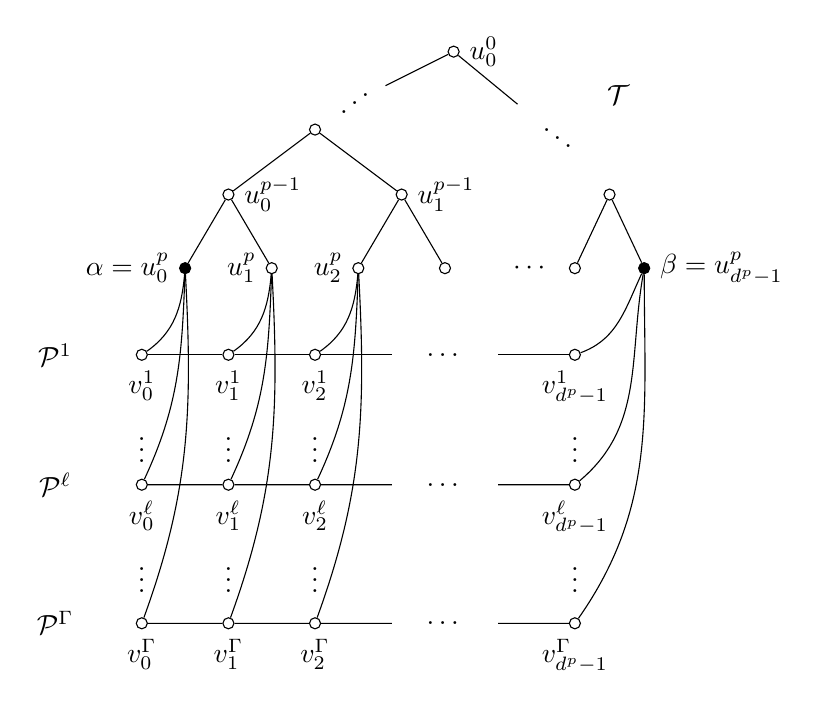
\begin{tikzpicture}[scale=1.1]
    % Define styles for different types of vertices
    \tikzset{
        vertex/.style={circle, draw, minimum size=4pt, inner sep=1pt, fill=white},
        filled/.style={circle, draw, fill=black, minimum size=4pt, inner sep=1pt},
    }
    
    
    % Draw vertices on level A with labels
    \node[] at (-1,0) {$\mathcal{P}^1$};
    \node[vertex] (a) at (0,0) [label=below:$v^1_0$] {};
    \node[vertex] (b) at (1,0) [label=below:$v^1_1$] {};
    \node[vertex] (c) at (2,0) [label=below:$v^1_2$] {};
    \node[] (ca) at (3,0) {};
    \node[] at (3.5,0) {$\dots$};
    \node[] (cb) at (4,0) {};
    \node[vertex] (d) at (5,0) [label=below:$v^1_{d^p-1}$] {};

    \node (dda) at (0,-1) {$\vdots$};
    \node (ddb) at (1,-1) {$\vdots$};
    \node (ddc) at (2,-1) {$\vdots$};
    \node (ddd) at (5,-1) {$\vdots$};
    \node (ddda) at (0,-2.5) {$\vdots$};
    \node (dddb) at (1,-2.5) {$\vdots$};
    \node (dddc) at (2,-2.5) {$\vdots$};
    \node (dddd) at (5,-2.5) {$\vdots$};
    
    % Draw vertices on level B with labels
    \node[] at (-1,-1.5) {$\mathcal{P}^\ell$};
    \node[vertex] (e) at (0,-1.5) [label=below:$v^\ell_0$] {};
    \node[vertex] (f) at (1,-1.5) [label=below:$v^\ell_1$] {};
    \node[vertex] (g) at (2,-1.5) [label=below:$v^\ell_2$] {};
    \node[] (ga) at (3,-1.5) {};
    \node[] at (3.5,-1.5) {$\dots$};
    \node[] (gb) at (4,-1.5) {};
    \node[vertex] (h) at (5,-1.5) [label=below:$v^\ell_{d^p-1}$] {};
    
    % Draw vertices on level C with labels
    \node[] at (-1,-3.1) {$\mathcal{P}^\Gamma$};
    \node[vertex] (i) at (0,-3.1) [label=below:$v^\Gamma_0$] {};
    \node[vertex] (j) at (1,-3.1) [label=below:$v^\Gamma_1$] {};
    \node[vertex] (k) at (2,-3.1) [label=below:$v^\Gamma_2$] {};
    \node[] (ka) at (3,-3.1) {};
    \node[] at (3.5,-3.1) {$\dots$};
    \node[] (kb) at (4,-3.1) {};
    \node[vertex] (l) at (5,-3.1) [label=below:$v^\Gamma_{d^p-1}$] {};
    
    % Draw tree structure vertices
    \node at (5.5,3) {$\mathcal{T}$};
    \node[vertex] (o) at (3.6,3.5) [label=right:$u_0^0$] {};
    
    \node (left) at (2.7,3.05) {};
    \node (right) at (4.45,2.8) {};
    
    \node (eleft) at (2.45,3) {$\iddots$};
    \node (eright) at (4.8,2.6) {$\ddots$};
    \node[vertex] (pq) at (2,2.6) {};
    
    \node[vertex] (p) at (1,1.85) [label=right:$u^{p-1}_0$] {};
    \node[vertex] (q) at (3,1.85) [label=right:$u^{p-1}_1$] {};
    \node[vertex] (qq) at (5.4,1.85) {};
    
    \node[filled] (s) at (0.5,1) [label=left:{$\alpha=u^p_0$}] {};
    \node[vertex] (m) at (1.5,1) [label=left:$u^p_1$] {};
    \node[vertex] (n) at (2.5,1) [label=left:$u^p_2$] {};
    \node[vertex] (nn) at (3.5,1) {};
    \node (mid) at (4.5,1) {$\cdots$};
    \node[vertex] (rl) at (5,1) {};
    \node[filled] (r) at (5.8,1) [label=right:{$\beta=u^p_{d^p-1}$}] {};
    
    % Draw path connections
    \draw (a) -- (b) -- (c) -- (ca);
    \draw (e) -- (f) -- (g) -- (ga);
    \draw (i) -- (j) -- (k) -- (ka);
    \draw (cb) -- (d);
    \draw (gb) -- (h);
    \draw (kb) -- (l);
    
    % Draw tree connections
    \draw (o) -- (left);
    \draw (o) -- (right);
    \draw (p) -- (pq);
    \draw (q) -- (pq);
    \draw (p) -- (s);
    \draw (p) -- (m);
    \draw (q) -- (n);
    \draw (q) -- (nn);
    \draw (qq) -- (r);
    \draw (qq) -- (rl);
    
    \draw (s) to [out=265, in=35] (a);
    \draw (s) to [out=268, in=65] (e);
    \draw (s) to [out=273, in=70] (i);
    \draw (m) to [out=265, in=35] (b);
    \draw (m) to [out=268, in=65] (f);
    \draw (m) to [out=273, in=70] (j);
    \draw (n) to [out=265, in=35] (c);
    \draw (n) to [out=268, in=65] (g);
    \draw (n) to [out=273, in=70] (k);
    \draw (r) to [out=245, in=20] (d);
    \draw (r) to [out=260, in=40] (h);
    \draw (r) to [out=270, in=55] (l);
\end{tikzpicture}
    \caption{An example of $\GGdp$ with $d=2$.}
    \label{fig:GGdp}
\end{figure}

We restate the simulation lemma of \citet{das2011distributed}, which connects the computation of Boolean function in the traditional communication complexity model to the computation of Boolean function in the distributed model in graph $\GGdp$ with input vertices $\alpha$ and $\beta$.


% \yanyu{maybe the lemma before the simulation lemma is also needed. (will add later if it's needed)}
\begin{lemma}[Simulation lemma \cite{das2011distributed}]
\label{thm:simulation}
For any $\Gamma$, $d$, $p$, $B$, $\epsilon\geq 0$, and function $f:\bin^b \times \bin^b \to \bin$, if there is an $\epsilon$-error randomized distributed algorithm that computes $f(x,y)$ faster than $\frac{d^p-1}{2}$ rounds on $\GGdp$ with $x$ given to vertex $\alpha$ and $y$ given to vertex $\beta$, i.e.,
$
R_\epsilon^{\GGdp}(f) < \frac{d^p-1}{2},
$
then there is an $\epsilon$-error randomized algorithm in the communication complexity model that computes $f$ using at most $2dpB R_\epsilon^{\GGdp}(f)$ bits of communication.
In other words,
$
R_\epsilon^{cc-pub}(f)\leq 2dpB R_\epsilon^{\GGdp}(f).
$
% \yijun{When I first read the theorem I found it very confusing. I think an important point that is missing is that you need to say how the input to the function $f$ is stored in the network.}
\end{lemma}
%\yijun{rounds in distributes setting, bits in communication complexity}

% The simulation lemma was proved by carefully analyzing the states of the distributed (sub)-network over rounds, and showing that only $O(dp)$ messages are needed for Alice and Bob to simulate one round of the execution of any distributed algorithm on $\GGdp$. Hence, Alice and Bob can perform the above simulation and run any distributed algorithm for computing functions on $\alpha$ and $\beta$ on $\GGdp$ in the communication complexity model with only $O(dp)$-factor overhead.

% \yijun{Some suggestions: 
% (1) Include a very brief proof idea for the simulation lemma. 
% (2) Include a very brief proof sketch (no theorems, just a paragraph) for how the simulation lemma is used to give $\Omega(\sqrt{n})$ for one problem. Otherwise, the reader might be very lost.
% }
% \yanyu{(1) above (2) below}
The simulation lemma was proved by analyzing the states of the distributed (sub)-network over rounds. In $\GGdp$, Alice and Bob have two ways to communicate $b$ bits: either through paths of length $d^p-1$ between them, or through the tree structure. When an algorithm's runtime is less than $(d^p-1)/2$, messages cannot traverse the full path between Alice and Bob, forcing communication through the tree structure. This creates a congestion bottleneck which is manifested by their analysis that only $O(dp)$ messages are needed to simulate all messages sent in each round of the distributed algorithm on $\GGdp$. This allows Alice and Bob to simulate any distributed algorithm for computing functions $f$ on $\alpha$ and $\beta$ on $\GGdp$ in the communication complexity model with an $O(dp)$-factor overhead.
%\yanyu{edited}
%\yijun{the paragraph above essentially conveys zero information... I would at least explain why the threshold $(d^p-1)/2$ makes sense: Essentially there are two ways for Alice and Bob to communicate $\Theta(d^p)$ bits of information to each other: via paths or via trees, the first suffers from a dilation of $\Theta(d^p)$, the second suffers from a congestion of $\Theta(d^p)$}

The main way the above simulation lemma is used is via the following lemma which applies the simulation lemma specifically for the $\disj$ function. It translates the lower bound for $\disj$ in the communication model to a lower bound for computing $\disj$ in $\GGdp$ on $\alpha$ and $\beta$. 

\begin{lemma}[Set disjointness lower bound for $\GGdp$~\cite{das2011distributed}]\label{lem:disj}
For any $\Gamma, d, p$, there exists a constant $\epsilon>0$ such that
$$R_\epsilon^{\GGdp}\left(\disj_b;B\right)=\Omega\left(\min\left(d^p, \frac{b}{dpB}\right)\right).$$
\end{lemma}






\subsection{Modification to \GGdptitle{}}
\label{subsec:modification}

In this section, we present our graph construction $\Gkdpp$ builds upon $\GGdp$ to allow us to perform a reduction from distributed set disjointness to the \secsisp{} and \rpath{} problems. Compared with the $\widetilde{\Omega}(\sqrt{n})$ lower bounds obtained via existing constructions~\cite{das2011distributed,manoharan2024computing}, our graph construction $\Gkdpp$ allows us to obtain a higher $\widetilde{\Omega}(n^{2/3})$ lower bound. 
%\yijun{the first sentence is a bit awkward}
We show how to simulate any distributed disjointness algorithm for $\Gkdpp$ on $\GGdp$ with $O(1)$-factor overhead. Connecting these two results, we obtain a lower bound for computing disjointness on $\Gkdpp$ with inputs given to $\alpha$ and $\beta$.

\paragraph{Intuition.} Our lower bound construction is built around a bipartite graph positioned at the far end of the structure, which controls the replacement path distances for each edge along the given $s$-$t$ path. We aim to establish a correspondence between the edge orientations in the bipartite graph and the replacement path distances for the edges in the given $s$-$t$ path. Moreover, we require that reversing the orientation of the edges in the bipartite graph result in longer replacement paths. To solve the replacement path problem, Alice must learn the orientation of every edge in the bipartite graph, requiring substantial information to be transmitted from one end to the other.
%\yanyu{edited}
% so that the length of the second simple shortest path, i.e. the minimum replacement path across all edges in the given $s$-$t$ path, can be used to indicate the disjointness between two parties. 
% \yanyu{is this confusing out of context?}
% \yijun{This is confusing because You only discuss $M$ and omit $x$ entirely. There are two ways to improve the writing: One is that here you just say that to solve replacement paths we need to learn all the edge orientations in the bipartite graphs (without mentioning \secsisp{} and set disjointness), requiring transmitting a lot of information from one end to the other end. Second is to include more detail of not only $M$ but also $x$ and say that they correspond to the set disjointness input and how they affect replacement path length (you can also choose to do this later in the place where you introduce them).}

The construction proceeds by first establishing a mapping between each edge on the $s$-$t$ path and its corresponding edge in the bipartite graph. 
For each edge in the $s$-$t$ path, we connect a long path to its mapped edge in the bipartite graph.
% to increase the distance between the given $s$-$t$ path and the bipartite graph where the direction information is stored. 
The long distance between the output vertices (vertices in the given $s$-$t$ path) and the location of critical information (edge orientations in the bipartite graph) forces the algorithm to spend more rounds propagating information to their required destinations. 
The orientation of the edges in the bipartite graph determines the length of the replacement path for their corresponding edges. %This correspondence is critical for computing disjointness. 
With $n^{1/3}$ paths of length approximately $n^{2/3}$, the algorithm requires at least $n^{2/3}$ rounds to propagate this critical information. 
Next, to reduce the graph's diameter without creating additional replacement paths, we incorporate a tree-like structure with downward edge orientations along the path. As demonstrated in the simulation lemma of \citet{das2011distributed} and our new simulation in \Cref{lem:disj G(kdpp)}, this structure does not substantially improve the propagation of critical information.
Finally, to optimize the total number of vertices, we carefully merge paths that lead to the same vertex in the bipartite graph while ensuring that the correspondence between edge orientations in the bipartite graph and replacement path lengths remains intact.
%\yanyu{edited}
% \yijun{I did not see the main idea being explicitly mentioned: the orientation of each edge in the bipartite graph controls the replacement path length for the corresponding edge (for one direction, you can use that in the replacement path, for the other direction, you need to take a longer detour), so the replacement path distance can be used to determine the direction of the corresponding edge in the bipartite graph. Therefore, solving the replacement path problem requires communicating $\Omega(n^{2/3})$ bits of information from one side of the graph to the other side of the graph.}


\paragraph{Construction of \Gkdpptitle.}
Our modified graph is called $\Gkdpp$ where $\phi: [k^2] \to [k]\times[k]$ is a bijection used to map any edge $\left(s_{i-1}, s_i\right)$ on the given $s$-$t$ path to an edge on the bipartite graph. Refer to \Cref{fig:Gkdpp} for an illustration. We present the construction of $\Gkdpp$ with some default edge orientation. %If the problem in consideration only concerns undirected graph, then ignore the default direction provided. [Yi-Jun: I commented out the above sentence as it seems irrelevant to us]
The graph $\Gkdpp$ is constructed via the following steps:
% \yijun{
% This is a complicated construction. Need to give intuition. Also, 
% try to give a proof sketch/idea before presenting the formal proofs in the next sub-section.}
\begin{enumerate}
    \item Construct $\GGdp$ with $\Gamma = 2k$. We relabel the vertices of the last $k$ paths by $w^\ell_i$, where $1\leq\ell\leq k$ and $0\leq i\leq d^p-1$. For $1\leq\ell\leq k$, we use the shorthand $v^\ell$ and $w^\ell$ to denote the \emph{last} vertex of path $\Pc^\ell$ and $\Pc^{\ell+k}$, respectively. 
    \item For $1\leq i,j \leq k$, add edges $\{v^i, w^j\}$.
    \item Add a directed path $\mathcal{P^*}$ with $k^2$ edges from $s$ to $t$.\\ We label the vertices on the path by $s=s_0, s_1, \dots, s_{k^2}=t$. 
    \item Add $k$ paths $\Qc^1, \dots, \Qc^k$ each of length $2k^2$, where $\Qc^\ell$ consists of vertices $q^\ell_0, \dots, q^\ell_{2k^2}$. \\For each $1\leq\ell\leq k$, add edge $\left(q^{\ell}_{2k^2}, v^{\ell}_0\right)$.
    \item Add $k$ paths $\Rc^1, \dots, \Rc^k$ each of length $2k^2$, where $\Rc^\ell$ consists of vertices $r^\ell_0, \dots, r^\ell_{2k^2}$. \\For each $1\leq\ell\leq k$, add edge $\left(w^{\ell}_0, r^{\ell}_{0}\right)$.
    \item For $i\in [k^2]$, suppose $\phi(i)=\left(\phi_1(i),\phi_2(i)\right)$, add $\left\{s_{i-1}, q^{\phi_1(i)}_{2(i-1)}\right\}$ and $\left(r^{\phi_2(i)}_{2i}, s_i\right)$.
    \item Add edges from $\alpha$ to all vertices in $\Pstar, \Qc^i, \Rc^i$, for each $1\leq i \leq k$.
\end{enumerate}

\paragraph{Direction of edges.}
To facilitate our reduction from set disjointness to \secsisp{}, we assigned default orientations for all edges in $\Gkdpp$ except for those in the right bipartite graph and edges of the form $\left\{s_{i-1}, q^{\phi_1(i)}_{2(i-1)}\right\}$. The direction of the edges on the bipartite graph is determined by a matrix $M\in \bin^{k\times k}$ and the direction of the edges $\left\{s_{i-1}, q^{\phi_1(i)}_{2(i-1)}\right\}$ are determined by a vector $x\in \bin^{k^2}$. The directed version of the graph $\GkdppMx$ is constructed as follows.

\begin{enumerate}
    \item Orient the edges in paths $\Pstar, \Pc^\ell, \Qc^\ell, \Rc^\ell$ pointing to larger index for $1\leq \ell \leq k$ and orient the edges in paths $\Pc^\ell$ pointing to smaller index for $k+1\leq \ell \leq 2k$.
    \item Orient the edges in the tree $\Tc$ from parents to children. Orient the edges between the leaves and the paths pointing away from the leaves.  
    \item For $1\leq i,j \leq k$, add edge $(v^i, w^j)$ if $M_{ij}=1$. Otherwise, add edge $(w^j, v^i)$.
    \item For $i\in [k^2]$, set direction as $\left(s_{i-1}, q^{\phi_1(i)}_{2(i-1)}\right)$ if $x_i = 1$. Otherwise, set direction as $\left(q^{\phi_1(i)}_{2(i-1)}, s_{i-1}\right)$.
\end{enumerate}

When $x_i = 1$, alternative paths avoiding $\left(s_{i-1}, s_i\right)$ can use the edge $\left(s_{i-1}, q^{\phi_1(i)}_{2(i-1)}\right)$ to make a detour. Conversely, when $x_i = 0$, any alternative paths avoiding $(s_{i-1}, s_i)$ must leave $\Pstar$ before $s_{i-1}$. Since the paths $\Qc^\ell$ have double the length, alternative paths exiting earlier will have longer lengths. If the corresponding edge in the bipartite graph is oriented as $\left(v^{\phi_1(i)}, w^{\phi_2(i)}\right)$ (i.e. when $M_{\phi_1(i), \phi_2(i)}=1$), the returning detour using the edge $\left(r^{\phi_2(i)}_{2i}, s_i\right)$ can be taken. For the same reason, detours returning earlier will have shorter lengths. Hence, the shortest detour is possible if and only if both $x_i = 1$ and $M_{\phi_1(i), \phi_2(i)}=1$, allowing us to reduce set disjointness to \secsisp{}.

%\yanyu{added motivation behind $M$ and $x$}
% \yijun{Now is the right place to explain the motivation behind $M$ and $x$: Say that they correspond to the set disjointness input, and intuitively how their values affect replacement path length.}
% Firstly, we consider $\Gamma = 2k$ and we relabel the vertices of the last $k$ path as $w^\ell_i$. Now, we add a directed path $\mathcal{P^*}$ with $k^2$ edges from $s$ to $t$. We label the vertices on the path by $s=s_0, s_1, \dots, t=s_{k^2}$. 
% Then consider a bijection $\phi: [k^2] \to [k]\times[k]$. Suppose $\phi(i) = (\phi(i)_1, \phi(i)_2)$, this bijection is used to map any edge $\left(s_{i-1}, s_i\right)$ on $\Pstar$ to a vertex pair $\left(v^{\phi(i)_1}, w^{\phi(i)_2}\right)$. 
% Then we further add $2k$ number of paths $\Qc^1, \dots, \Qc^k$ and $\Rc^1, \dots, \Rc^k$, each having $2k^2$ edges, with vertices indexed from $0$ to $2k^2$. For each $1\leq\ell\leq k$, add edges $\left(q^{\ell}_{2k^2}, v^{\ell}_0\right)$ and $\left(w^{\ell}_0, r^{\ell}_{0}\right)$
% For each edge $(s_{i-1}, s_i)$, add $\left(s_{i-1}, q^{\phi(i)_1}_{2(i-1)}\right)$ and $\left(r^{\phi(i)_2}_{2i}, s_i\right)$. Lastly, we add edges from $\alpha$ to all vertices on $\Pstar, \Qc^i, \Rc^i$.


\begin{figure}[ht!]
    \centering
    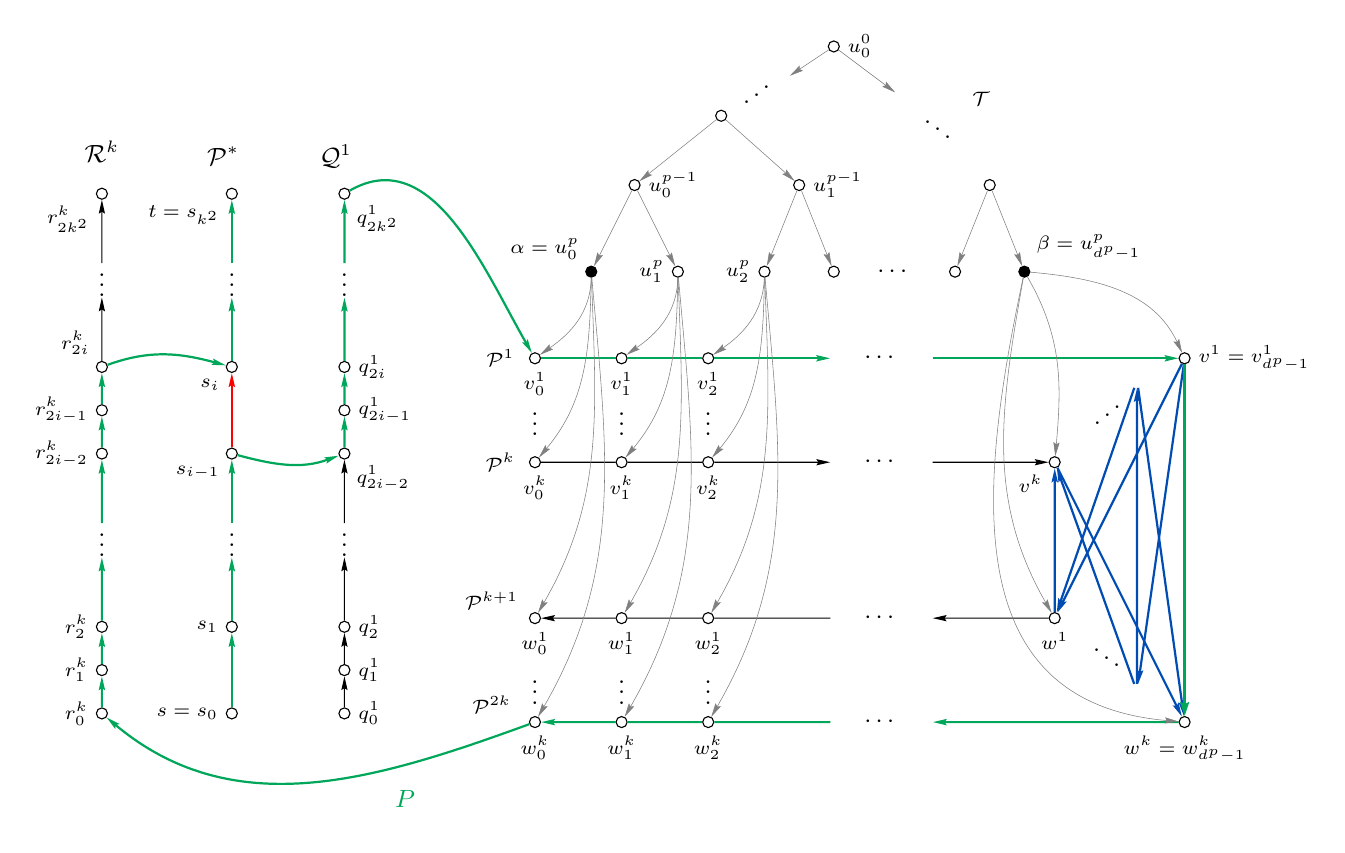
\begin{tikzpicture}[scale=1.1]
\scriptsize
    % Define styles for different types of vertices
    \tikzset{
        vertex/.style={circle, draw, minimum size=4pt, inner sep=1pt, fill=white},
        filled/.style={circle, draw, fill=black, minimum size=4pt, inner sep=1pt},
        symbol/.style={inner sep=0pt, font=\small, text height=12pt},
        small/.style={font=\small},
        mapping/.style={teal!60!blue, thick},
        dir/.style={arrows = {-Stealth[inset=0.7pt, length=5pt, angle'=25]}},
        widedir/.style={arrows = {-Stealth[inset=0.7pt, length=5pt, angle'=35]}},
        highlight/.style={teal!70!green, thick},
        hlar/.style={highlight, dir},
        line/.style={gray, very thin, dir},
    }
    
    % Draw vertices on level A with labels
    \node[] at (-0.4,0) {$\mathcal{P}^1$};
    \node[vertex] (a) at (0,0) [label=below:$v^1_0$] {};
    \node[vertex] (b) at (1,0) [label=below:$v^1_1$] {};
    \node[vertex] (c) at (2,0) [label=below:$v^1_2$] {};
    \node[] (ca) at (3.5,0) {};
    % \node[] (ca2) at (3.5,0) {};
    \node[small] at (4,0) {$\cdots$};
    \node[] (cb) at (4.5,0) {};
    \node[vertex] (d) at (7.5,0) [label=right:{$v^1=v^1_{d^p-1}$}] {};

    \node[symbol] (dda) at (0,-0.7) {$\vdots$};
    \node[symbol] (ddb) at (1,-0.7) {$\vdots$};
    \node[symbol] (ddc) at (2,-0.7) {$\vdots$};
    \node[symbol] (ddd) at (6.6,-0.6) {$\iddots$};
    
    \node[symbol] (ddda) at (0,-3.8) {$\vdots$};
    \node[symbol] (dddb) at (1,-3.8) {$\vdots$};
    \node[symbol] (dddc) at (2,-3.8) {$\vdots$};
    \node[symbol] (dddd) at (6.6,-3.4) {$\ddots$};
    
    % Draw vertices on level B with labels
    \node[] at (-0.4,-1.2) {$\mathcal{P}^k$};
    \node[vertex] (e) at (0,-1.2) [label=below:$v^k_0$] {};
    \node[vertex] (f) at (1,-1.2) [label=below:$v^k_1$] {};
    \node[vertex] (g) at (2,-1.2) [label=below:$v^k_2$] {};
    \node[] (ga) at (3.5,-1.2) {};
    \node[small] at (4,-1.2) {$\cdots$};
    \node[] (gb) at (4.5,-1.2) {};
    \node[vertex] (h) at (6,-1.2) [label=below left:{$v^k$}] {};

    % Draw vertices on level C with labels
    \node[] at (-0.5,-2.8) {$\mathcal{P}^{k+1}$};
    \node[vertex] (e2) at (0,-3) [label=below:$w^1_0$] {};
    \node[vertex] (f2) at (1,-3) [label=below:$w^1_1$] {};
    \node[vertex] (g2) at (2,-3) [label=below:$w^1_2$] {};
    \node[] (ga2) at (3.5,-3) {};
    \node[small] at (4,-3) {$\cdots$};
    \node[] (gb2) at (4.5,-3) {};
    \node[vertex] (h2) at (6,-3) [label=below:{$w^1$}] {};
    
    
    % Draw vertices on level D with labels
    \node[] at (-0.5,-4) {$\mathcal{P}^{2k}$};
    \node[vertex] (i) at (0,-4.2) [label=below:$w^k_0$] {};
    \node[vertex] (j) at (1,-4.2) [label=below:$w^k_1$] {};
    \node[vertex] (k) at (2,-4.2) [label=below:$w^k_2$] {};
    \node[] (ka) at (3.5,-4.2) {};
    \node[small] at (4, -4.2) {$\cdots$};
    \node[] (kb) at (4.5,-4.2) {};
    \node[vertex] (l) at (7.5,-4.2) [label=below:{$w^k=w^k_{d^p-1}$}] {};
    
    % Draw tree structure vertices
    \begin{scope}[xshift=1.5mm, yshift=0mm]
        \node at (5,3) {$\mathcal{T}$};
        \node[vertex] (o) at (3.3,3.6) [label=right:$u_0^0$] {};
        
        \node (left) at (2.7,3.2) {};
        \node (right) at (4.1,3.0) {};
        
        \node[symbol] (eleft) at (2.4,3.1) {$\iddots$};
        \node[symbol] (eright) at (4.5,2.7) {$\ddots$};
        \node[small] (mid) at (4,1) {$\cdots$};
        \node[vertex] (pq) at (2,2.8) {};
        
        \node[vertex] (p) at (1,2) [label=right:$u^{p-1}_0$] {};
        \node[vertex] (q) at (2.9,2) [label=right:$u^{p-1}_1$] {};
        \node[vertex] (qq) at (5.1,2) {};
        
        \node[filled] (s) at (0.5,) [label=above left:{$\alpha=u^p_0$}] {};
        \node[vertex] (m) at (1.5,1) [label=left:$u^p_1$] {};
        \node[vertex] (n) at (2.5,1) [label=left:$u^p_2$] {};
        \node[vertex] (nn) at (3.3,1) {};
        \node[vertex] (rl) at (4.7,1) {};
        \node[filled] (r) at (5.5,1) [label=above right:{$\beta=u^p_{d^p-1}$}] {};
    \end{scope}
    % Draw path connections
    \draw[dir, highlight] (a) -- (b) -- (c) -- (ca);
    \draw[dir] (e) -- (f) -- (g) -- (ga);
    \draw[dir] (ga2) -- (g2) -- (f2) -- (e2);
    \draw[dir, highlight] (ka) -- (k) -- (j) -- (i);
    \draw[dir, highlight] (cb) -- (d);
    \draw[dir] (gb) -- (h);
    \draw[dir] (h2) -- (gb2);
    \draw[dir, highlight] (l) -- (kb);
    
    % Draw tree connections
    \draw[line] (o) -- (left);
    \draw[line] (o) -- (right);
    \draw[line] (pq) -- (p);
    \draw[line] (pq) -- (q);
    \draw[line] (p) -- (s);
    \draw[line] (p) -- (m);
    \draw[line] (q) -- (n);
    \draw[line] (q) -- (nn);
    \draw[line] (qq) -- (r);
    \draw[line] (qq) -- (rl);
    
    \draw[line] (s) to [out=269,in=35] (a);
    \draw[line] (s) to [out=269,in=50] (e);
    \draw[line] (s) to [out=272,in=60] (e2);
    \draw[line] (s) to [out=275,in=60] (i);
    
    \draw[line] (m) to [out=269,in=35] (b);
    \draw[line] (m) to [out=269,in=50] (f);
    \draw[line] (m) to [out=272,in=60] (f2);
    \draw[line] (m) to [out=275,in=60] (j);
    
    \draw[line] (n) to [out=268,in=35] (c);
    \draw[line] (n) to [out=269,in=50] (g);
    \draw[line] (n) to [out=272,in=60] (g2);
    \draw[line] (n) to [out=275,in=60] (k);
    
    \draw[line] (r) to [out=355,in=115] (d);
    \draw[line] (r) to [out=300,in=85] (h);
    \draw[line] (r) to [out=260,in=120, looseness=1] (h2);
    \draw[line] (r) to [out=258,in=175, looseness=1.2] (l);

    % Bipartite graph mapped from the string y
    \node (vl) at (6.95,-0.25) {};
    \node (wl) at (6.95,-3.85) {};
    \draw[dir, mapping] (d) -- (h2);
    \draw[dir, mapping] (d) -- (wl);
    \draw[dir, mapping] (vl) -- (l);
    \draw[dir, mapping] (wl) -- (vl);
    \draw[dir, mapping] (vl) -- (h2);
    \draw[dir, mapping] (h) -- (l);
    \draw[dir, mapping] (h2) -- (h);
    \draw[dir, mapping] (wl) -- (h);
    \draw[widedir, highlight, very thick] (d) -- (l);

    \begin{scope}[xshift=-35mm, yshift=-1mm]
        \node[vertex] (s0) at (0,-4) [label=left:{$s=s_0$}] {};
        \node[vertex] (s1) at (0,-3) [label=left:$s_1$] {};
        \node[symbol] (s2) at (0,-2) {$\vdots$};
        \node[vertex] (sj) at (0,-1) [label=below left:$s_{i-1}$] {};
        \node[vertex] (si) at (0,0) [label=below left:$s_i$] {};
        \node[symbol] (s5) at (0,1) {$\vdots$};
        \node[vertex] (st) at (0,2) [label=below left:{$t=s_{k^2}$}] {};
        \node[symbol] (Pstar) at (-0.1,2.52)  {$\mathcal{P}^*$};

        \draw[dir, highlight] (s0) -- (s1);
        \draw[dir, highlight] (s1) -- (s2);
        \draw[dir, highlight] (s2) -- (sj);
        \draw[dir, red, thick] (sj) -- (si);
        \draw[dir, highlight] (si) -- (s5);
        \draw[dir, highlight] (s5) -- (st);

        \node[symbol] (Q)  at (1.2,2.5)    {$\mathcal{Q}^1$};
        \node[vertex] (q0)  at (1.3,-4)     [label=right:{$q^1_0$}] {};
        \node[vertex] (q05) at (1.3,-3.5) [label=right:{$q^1_1$}] {};
        \node[vertex] (q1)  at (1.3,-3)    [label=right:{$q^1_2$}] {};
        \node[symbol] (q2)  at (1.3,-2) {$\vdots$};
        \node[vertex] (qj)  at (1.3,-1)    [label=below right:$q^1_{2i-2}$]{};
        \node[vertex] (qji) at (1.3,-0.5) [label=right:$q^1_{2i-1}$]{};
        \node[vertex] (qi)  at (1.3,0)     [label=right:$q^1_{2i}$] {};
        \node[symbol] (q5)  at (1.3,1) {$\vdots$};
        \node[vertex] (qt)  at (1.3,2)     [label=below right:{$q^1_{2k^2}$}] {};

        \draw[dir] (q0)  -- (q05);
        \draw[dir] (q05) -- (q1);
        \draw[dir] (q1)  -- (q2);
        \draw[dir] (q2)  -- (qj);
        \draw[dir, highlight] (qj)  -- (qji);
        \draw[dir, highlight] (qji) -- (qi);
        \draw[dir, highlight] (qi)  -- (q5);
        \draw[dir, highlight] (q5)  -- (qt);

        \node[symbol] (r)  at (-1.5,2.55)    {$\mathcal{R}^k$};
        \node[vertex] (r0)  at (-1.5,-4)    [label=left:{$r^k_0$}] {};
        \node[vertex] (r05) at (-1.5,-3.5)  [label=left:{$r^k_1$}] {};
        \node[vertex] (r1)  at (-1.5,-3)    [label=left:{$r^k_2$}] {};
        \node[symbol] (r2)  at (-1.5,-2) {$\vdots$};
        \node[vertex] (rj)  at (-1.5,-1)    [label=left:$r^k_{2i-2}$]{};
        \node[vertex] (rji) at (-1.5,-0.5)  [label=left:$r^k_{2i-1}$]{};
        \node[vertex] (ri)  at (-1.5,0)     [label=above left:$r^k_{2i}$] {};
        \node[symbol] (r5)  at (-1.5,1) {$\vdots$};
        \node[vertex] (rt)  at (-1.5,2)     [label=below left:{$r^k_{2k^2}$}] {};

        \draw[dir, highlight] (r0)  -- (r05);
        \draw[dir, highlight] (r05) -- (r1);
        \draw[dir, highlight] (r1)  -- (r2);
        \draw[dir, highlight] (r2)  -- (rj);
        \draw[dir, highlight] (rj)  -- (rji);
        \draw[dir, highlight] (rji) -- (ri);
        \draw[dir] (ri)  -- (r5);
        \draw[dir] (r5)  -- (rt);
        
        \draw[hlar] (ri)  to [out=20,in=165] (si);
        \draw[hlar] (sj)  to [out=345,in=200] (qj);
    \end{scope}

    \draw[dir, highlight] (qt)  to [out=30,in=120] (a);
    \draw[dir, highlight] (i)  to [out=200,in=320] (r0);
    \node[symbol] (PPP)  at (-1.5,-5) {{\color{teal!70!green}$P$}};
\end{tikzpicture}
    \caption{Illustration of $\Gkdpp$, assuming $\phi(i)=(1,k)$ and $M_{1,k} = 1$. Paths $\Qc^2,\dots,\Qc^k$ and $\Rc^1,\dots,\Rc^{k-1}$ are omitted. Other edges from $\Pstar$ to $\Qc^1$, and from $\Rc^k$ to $\Pstar$ are omitted. Edges from $\alpha$ to $\Pstar, \Qc^i$ and $\Rc^i$ are omitted. Reversed directional edges in the bipartite graph are omitted. When $(v^1, w^k)$ is oriented correctly, the green highlighted path $P$ is a replacement path from $s$ to $t$ for the deleted edge $(s_{i-1}, s_i)$.}
    \label{fig:Gkdpp}
\end{figure}

\begin{observation}[Basic properties of $\Gkdpp$]\label{obs:Gkdpp}
    There are $\Theta(k^3 + k d^p)$ vertices in $\Gkdpp$, and the diameter of $\Gkdpp$ is at most $2p+2$.
\end{observation}
    % \yijun{add a very short proof: especially the diameter part.}

\begin{proof}
    The number of vertices for the respective parts are: $2k d^p$ vertices for $\Pc^\ell$, $2k \times (2k^2+1)$ for $\Rc^\ell$ and $\Qc^\ell$, $k^2+1$ vertices for $\Pstar$ and $\frac{d^{p+1}-1}{d-1}$ vertices for $\Tc$. Hence the total number of vertices is $2k d^p +4k^3 + 2k + k^2 + 1 + \frac{d^{p+1}-1}{d-1} = \Theta(k^3+kd^p)$. Every vertex not on the tree $\Tc$ is connected to some leaf in $\Tc$. Since $\Tc$ has depth $p$, the diameter of $\Gkdpp$ is at most $2p+2$.
\end{proof}
    
Now we show a lemma for a lower bound of distributed algorithms for set disjointness on $\Gkdpp$. This is analogous to \Cref{lem:disj}. We achieve this by applying \Cref{thm:simulation} and \Cref{lem:disj} in a black-box manner, and showing how distributed algorithms for set disjointness on $\Gkdpp$ can be simulated on $\GGdp$ with $O(1)$-factor overhead. The intuition for the simulation is that $\alpha$ will simulate the vertices in $\Pstar, \Qc^\ell$ and $\Rc^\ell$ and $\beta$ will simulate the vertices in the bipartite graph. 


% \begin{theorem}[simulation lemma II]
% \label{thm:simulation G(kdpp)}
% For any $k$, $d$, $p$, $B$, bijection $\phi: [k^2]\to [k]\times [k]$ and matrix $M \in \bin^{k\times k}$,
% any $T$-round distributed algorithm $\Ac$ on $\Gkdpp$ can be simulated in $\GGdp$, with $\Gamma=2k$ in $3T$ rounds.
% \end{theorem}
% \yanyu{do we need to say what do we mean by ``simulate'' or is it clear in this context?}
% \yijun{I think you can avoid this issue by removing this theorem and incorporating the proof into the lemma below.}


% \begin{proof}
    
% \end{proof}


\begin{lemma}[Set disjointness lower bound for $\Gkdpp$]
\label{lem:disj G(kdpp)}
    For any $k, d, p$ and bijection $\phi: [k^2]\to [k]\times [k]$ there exists a constant $\epsilon>0$ such that
    $$R_\epsilon^{\Gkdpp}\left(\disj_b;B\right)=\Omega\left(\min\left(d^p, \frac{b}{dpB}\right)\right).$$
\end{lemma}

\begin{proof}
    First, we show that if there is a $T$-round distributed algorithm for set disjointness $\Ac$ on $\Gkdpp$, then there is a $3T$-round distributed algorithm for set disjointness on $\GGdp$. We achieve this via simulating $\Ac$ on $\GGdp$.

    Suppose we have an algorithm $\Ac$ on graph $\GkdppMx$, we will denote a message sent in the $i$th round of $\Ac$ from vertex $u$ to vertex $v$ as $\Mc_i(u\to v)$. 
    Now $\alpha$ in $\GGdp$ can simulate all the vertices in $\Rc^\ell, \Qc^\ell$ and $\Pstar$ in the following way. 
    vertex $\alpha$ will run $2k+2$ processes and run $\Ac$ for $\alpha, \Rc^\ell, \Qc^\ell$ and $\Pstar$ for $1\leq \ell \leq k$ on these processes. 
    Any messages among the vertices in $\alpha, \Rc^\ell, \Qc^\ell$ and $\Pstar$ can be handled locally between the processes.
    The only messages left are between $v^\ell_0$ and $q^\ell_{2k^2}$ and between $w^\ell_0$ and $r^\ell_0$, where $1\leq \ell\leq k$. For each $1\leq \ell\leq k$, $\Mc_i(q^\ell_{2k^2}\to v^\ell_0)$ and $\Mc_i(v^\ell_0 \to q^\ell_{2k^2})$ are delivered along the edge $\{q^\ell_{2k^2}, v^\ell_0\}$. Similarly, $\Mc_i(r^\ell_{0}\to w^\ell_0)$ and $\Mc_i(w^\ell_0 \to r^\ell_{0})$ are delivered along the edge $\{r^\ell_{0}, w^\ell_0\}$.  
    Since there are at most twice the number of messages along the edges of $\alpha$, we can simulate $\Ac$ on $\GGdp$ in $3T$ rounds.

    Now we describe how to handle the bipartite graph in $\GkdppMx$ in vertex $\beta$ on $\GGdp$. vertex $\beta$ will create $2k+1$ processes that run $\Ac$ acting as $\beta, v^\ell$ and $w^\ell$ locally, where $1\leq \ell\leq k$. Any messages among these vertices are handled locally on $\beta$. The only messages left are between $v^\ell_{d^p-2}$ and $v^\ell$ and between $w^\ell_{d^p-2}$ and $w^\ell$. We will focus on $v^\ell$ now since the behaviors on $w^\ell$ are similar. In the $(3i-2)$th round, vertex $v^\ell_{d^p-2}$ and $v^\ell$ exchange $\Mc_i(v^\ell_{d^p-2}\to v^\ell)$ and $\Mc_i(v^\ell\to v^\ell_{d^p-2})$. In the $(3i-1)$th round, $v^\ell$ relay $\Mc_i(v^\ell_{d^p-2}\to v^\ell)$ to $\beta$. $\beta$ now has all the information needed to compute $\Mc_{i+1}(v^\ell \to v^\ell_{d^p-2})$ locally. $\beta$ computes $\Mc_{i+1}(v^\ell \to v^\ell_{d^p-2})$ and send it to $v^\ell$ in the $3i$th round. Now $v^\ell$ has $\Mc_{i+1}(v^\ell \to v^\ell_{d^p-2})$ to send to $v^\ell_{d^p-2}$ in the $(3(i+1)-2)$th round and the process repeats.

    All other vertices in $\GGdp$ will execute their part of $\Ac$ with $2$ empty rounds between any two rounds in $\Ac$ to align their pace with that of vertices $\alpha$ and $\beta$.
    In this way, we can simulate any $T$-round algorithm on $\GkdppMx$ with $3T$ rounds on $\GGdp$.
    
    After applying \Cref{lem:disj}, we have the desired lower bound.
\end{proof}


\subsection{Lower Bound for the \secsisp{} Problem}
\label{subsec:lower bound reduction}
%\yijun{Shorten title name}
Now we are ready to show our main results: lower bounds for the \secsisp{} problem and the \rpath{} problem. We will show \Cref{thm:2sisp lower} by a reduction from the disjointness problem on $\Gkdpp$.
Before we show a reduction from disjointness to \secsisp{}, we show a correspondence between the replacement path lengths and the edge orientations in the bipartite graph.

\begin{lemma}[Replacement path lengths]
\label{lem:GkdppMx Rpath-dir correspondence}
    Consider the graph $\GkdppMx$. For any edge $(s_{i-1},s_i)$ in the path $\Pstar$, if $M_{\phi_1(i), \phi_2(i)}=1$ and $x_i=1$, the length of the replacement path is $3k^2 + 2 d^p + 6$. Otherwise, the length is strictly greater.
\end{lemma}

\begin{proof}
    Suppose $M_{\phi_1(i), \phi_2(i)}=1$ and $x_i = 1$, then the highlighted path $P$ as shown in \Cref{fig:Gkdpp} is an alternative path. It can be easily checked that it has length $3k^2 + 2 d^p + 6$. Now we show that it is the shortest among all alternative $s$-$t$ path. Observe that all alternative $s$-$t$ path must be of the form 
    $$s, \dots, s_{j-1}, q^{\phi_1(j)}_{2j-2}, \dots, q^{\phi_1(j)}_{2k^2}, \;\Pc^{\phi_1(j)},\; \Pc^{\phi_2(l)+k}, \;r^{\phi_2(l)}_0, \dots, r^{\phi_2(l)}_{2l}, s_l,\dots, t$$ where $j\leq i$ and $l\geq i$. 
    Notice that the length of the above path is $3k^2 + 2d^p + 4 + 2(l-j+1)$. This length is minimized when $l=j=i$ and we have our highlight path $P$ with length $3k^2 + 2 d^p + 6$.

    Conversely, suppose $M_{\phi_1(i), \phi_2(i)}=0$ or $x_i=0$. If $M_{\phi_1(i), \phi_2(i)}=0$, the shortest alternative path is has length greater than $3k^2 + 2 d^p + 6$. This is because, the choice of $j=l=i$ does not constitute a directed path anymore as the bipartite edge is oriented from $w^{\phi_2(i)}$ to $v^{\phi_1(i)}$. If $x_i=0$, then the alternate $s$-$t$ path must exit $\Pstar$ before $s_{i-1}$ and therefore has length greater than $3k^2 + 2 d^p + 6$.
\end{proof}

% \yijun{I think the proof of the lemma below is ok now (up to some minor typos).}
\begin{lemma}[Reducing set disjointness to \secsisp{}]\label{lem:Disj to 2sisp}
    For any $k$, $d\geq 2$, $p$, bijection $\phi: [k^2]\to [k]\times [k]$ and $\epsilon\geq 0$, if there exists an $\epsilon$-error randomized distributed algorithm for the \secsisp{} problem on graph $\GkdppMx$ for any $M\in \bin^{k\times k}$ and any $x\in \bin^{k^2}$ then there exists an $\epsilon$-error randomized algorithm for computing $\disj_{k^2}(x,y)$ (on $k^2$-bit inputs) on $\Gkdpp$ that uses the same round complexity with additional $O(\frac{k}{B})$ rounds.
\end{lemma}

\begin{proof}
    Suppose $\Ac$ is an $\epsilon$-error randomized distributed algorithm for the \secsisp{} problem and suppose we are given a set disjointness instance with $k^2$-bit strings on $\Gkdpp$. We aim to use $\Ac$ to solve the set disjointness problem $\disj_{k^2}(x,y)$.

    Suppose Alice received $x\in \bin^{k^2}$ on vertex $\alpha$ and Bob received $y\in \bin^{k^2}$ on vertex $\beta$. By viewing $y$ as a matrix $M$ (using the lexicographical map) and viewing input $x$ as the argument $x$ in $\GkdppMx$, Alice will orient the edges of the form $\left\{s_{i-1}, q^{\phi_1(i)}_{2(i-1)}\right\}$, and Bob will orient the edges in the bipartite graph to make $\GkdppMx$. Alice only needs to send one bit to each vertex in $\Pstar$. Bob will need to send $k$ bits of information to each of the $2k$ vertices, $v^1,\dots, v^k, w^1,\dots, w^k$. This will take $O(k/B)$ rounds. 
    % \yanyu{should be ok since $k$ is roughly $n^{1/3}$.}
    
   Alice and Bob, together with other vertices, run $\Ac$ on $\GkdppMx$. By \Cref{lem:GkdppMx Rpath-dir correspondence}, the length of the replacement path for each edge $(s_{i-1},s_i)$ is $3k^2 + 2 d^p + 6$ if $M_{\phi_1(i), \phi_2(i)}=1$ and $x_i=1$ and longer otherwise. Since the length of the second simple shortest path is the minimum replacement path across all edges on the shortest path, the length of the second simple shortest path is $3k^2 + 2 d^p + 6$ if and only if there is an index $i\in [k^2]$ such that $M_{\phi_1(i), \phi_2(i)}=1$ and $x_i=1$. Hence, Alice and Bob will output $0$ for $\disj_{k^2}(x,y)$ if and only if the length of the second simple shortest path is $3k^2 + 2 d^p + 6$. The failure probability follows directly.
    % Alice can gather the replacement path length for each edge and compute the matrix $M$ and hence the string $y$. Finally, Alice can compute the inner product $\inprod{x}{y}$ and send it to Bob via the tree $\Tc$ which takes $2p$ time. Due to the correspondence shown in \Cref{lem:GkdppMx Rpath-dir correspondence}, %\yijun{I don't understand the argument here. I know $y$ is $M$. What is $x$?}\yanyu{$x \in \bin^{k^2}$, just using inner product to say ``compute disjointness''}
    % Alice can compute $y$ correctly with probability $1-\epsilon$ as long as $\Ac$ succeeds with probability $1-\epsilon$. Hence, Alice and Bob can compute $\disj_{k^2}(x,y)$ on $\Gkdpp$ with probability at least $1-\epsilon$ given $\Ac$.
    % \yanyu{what is the difference between ``solve'', ``compute'', ``verify'' disjointness?}
    % \yijun{I would say that solve and compute are the same. Verify seems to be completely different: We are given a solution and we want to check whether it is correct. E.g., for NP-complete problems, verify is easy but solve is not (known to be) easy.}
    % \yanyu{Yes, I understand this in general, but for disjointness, we are asked to "compute" the disjointness right? Why is it verify? are we given the solution of the disjointness problem? that is either yes or no.}\yijun{Yes, so compute should be correct and verify is not correct (I think in a previous version I saw that you wrote verify at some places so I got confused)}
\end{proof}



\rpathlower*

\begin{proof}[Proof of \Cref{thm:2sisp lower}]
    \Cref{lem:disj G(kdpp)} provides a lower bound for distributed algorithms for computing disjointness on $\Gkdpp$ with input nodes $\alpha$ and $\beta$. Applying the reduction with additive $O(\frac{k}{B})$ overhead from disjointness to \secsisp{} in \Cref{lem:Disj to 2sisp}, we know that for any $k,d,p$, there exists a constant $\epsilon>0$ such that any algorithm for the \secsisp{} problem requires $$\Omega\Bigg(\min\left(d^p, \frac{k^2}{dpB}\right) - \frac{k}{B}\Bigg)$$ rounds in the $\CONGEST(B)$ model on some $\Theta(k^3 + k d^p)$-vertex graph with diameter $2p+2$, by \Cref{obs:Gkdpp}. %\yanyu{edited}

    % If we choose $k^2=d^{p+1} pB$, $\Omega\left(\min\left(d^p, \frac{k^2}{dpB}\right)\right) = \Omega\left(d^p\right)$. Since $\Gkdpp$ has $\Theta(k^3 + k d^p)$ vertices, $n = \Theta(k^3 + k d^p)$ and $\Omega\left(d^p\right) = \Omega\left(\TODO\right)$ 
    % \yanyu{I could not solve for a nice expression here. This is supposed to be better than the next paragraph.}\yijun{No need to find a nice expression. It is good as long as you can give $\Omega(n^{2/3})$ lower bound for infinitely many $n$ (on small diameter graphs).}

    We set $k^2=d^p$ and rewrite the lower bound in terms of the number of vertices in $\Gkdpp$, $n = \Theta\left(k^3 + k d^p\right) = \Theta\left((d^p)^{3/2}\right)$, as follows:
    %Since $\Gkdpp$ has $\Theta\left(k^3 + k d^p\right)$ vertices, $n = \Theta\left(k^3 + k d^p\right) = \Theta\left((d^p)^{3/2}\right)$. The lower bound then becomes 
    \[\Omega\left(\min\left(d^p, \frac{k^2}{dpB}\right)  - \frac{k}{B}\right) = \Omega\left(\frac{k^{2-2/p}}{pB} - \frac{k}{B}\right)= \Omega\left(\frac{(n/2)^{(2/3)(1-1/p)}}{pB}\right)= \Omega\left(\frac{n^{2/3}}{B\log n}\right).\qedhere\]
    % \yanyu{is it okay if for each diameter, their is only a constant number of graphs for such lower bound? In the previous paper, for each diameter, they have a infinite number of graphs for that lower bound.}
\end{proof}




\section{Approximation Algorithm for Weighted Directed Graphs}
\label{sec:wapprox}

In this section, we show an $\widetilde{O}(n^{2/3}+D)$-round randomized algorithm for the $(1+\epsilon)$-\apxrpath{} problem in weighted directed graphs. We assume that all the edge weights are positive integers in the range $[W]$, where $W = \poly(n)$ is polynomial in $n$. 

%In the weighted case, we define a detour path to be short if it consists of at most $k=n^{\frac23}$ hops.\yijun{Note: the short detour algorithm might output some detours exceeding this number of hops} Again, let $s = v_1, v_2, \dots, v_L=t$ be the vertices along $P$. The case handling long detour replacement paths remains mostly unchanged, so we will focus on the short detour replacement path case.%\yijun{Still need to have a lemma capturing the long detour case with a proof explaining how to adapt the approach for the unweighted case to the weighted approximation case}


As mentioned earlier, we can handle long-detour replacement paths similarly to the unweighted case. Thus, our focus will primarily be on short-detour replacement paths. We aim to prove the following result, where we still use $\zeta = n^{2/3}$ as the threshold.


\begin{proposition}[Short detours]\label{approx_short}
    For weighted directed graphs, for any constant $\epsilon \in (0,1)$, there exists an $\widetilde{O}(n^{2/3}+D)$-round deterministic algorithm that lets the first endpoint $v_i$ of each edge $e=(v_i, v_{i+1})$ in $P$ compute a number $x$ such that
    \[|st \diamond e| \leq x \leq (1+\epsilon) \cdot \text{the shortest replacement path length for $e$ with a short detour}.\] 
    %For any constant $\epsilon \in (0,1)$, there exists an $\widetilde{O}(n^{2/3}+D)$-round randomized algorithm that stores  $(1+\epsilon)$ approximation  of the length of the replacement paths $st \diamond (v_i,v_{i+1})$ with long detours in $v_i$ weighted directed graphs with high probability.
\end{proposition}

Similar to the statement of \Cref{Thm: Long Detour Part Works}, \Cref{approx_short} guarantees an $(1+\epsilon)$ approximation of the value of $|st \diamond e|$ only when some shortest replacement path for $e$ takes a short detour. Otherwise, \Cref{approx_short} provides only an upper bound on $|st \diamond e|$. 

\paragraph{Notations.} We further generalize the definition of $X[\cdot,\cdot]$ in \Cref{sec:short} to capture any two specified sets for possible starting points and ending points. Let $A$ and $B$ be two non-empty sets of integers such that $\max A < \min B$, define $X(A,B)$ as the length of a shortest replacement path with a short detour that starts from a vertex $v_i$ in $P$ with $i \in A$ and ends at a vertex $v_j$ in $P$ with $j \in B$. We define $Y(A,B)$ in the same way but without the requirement that the detour is short. Given a parameter $\epsilon \in (0,1)$, we say that a number $x$ is a \emph{good approximation} of $X(A,B)$ if it satisfies
\[Y(A,B) \leq x \leq (1+\epsilon)X(A,B).\]
For notational simplicity, we may write $\widetilde{X}(A,B)$ to denote a good approximation of $X(A,B)$.
Using the above terminology, the goal of \Cref{approx_short} is to let each vertex $v_i$ compute a good approximation of $X((-\infty,i], [i+1, \infty))$.


\paragraph{Hop-constrained BFS.} Recall that, for the \emph{unweighted} case, by doing a $\zeta$-hop \emph{backward} BFS from each vertex $v_i$ in the path $P$, with some branches trimmed, in $O(\zeta)$ rounds we can let each vertex $v_i$ calculate the \emph{exact} value of $X(\{i\}, [j, \infty))$ for all $j > i$.

A natural attempt to adapt this approach to the \emph{weighted} case is to replace hop-constrained BFS with hop-constrained shortest paths. However, we face a severe congestion issue that even with a hop constraint, all the $h_{st}-1$ shortest paths trees can potentially overlap at one edge. To overcome this issue, we apply a \emph{rounding} technique to reduce the weighted case to the unweighted case, so that we can directly apply the same backward BFS algorithm of \Cref{Thm: Backward BFS Works} to let each vertex $v_i$ obtain a \emph{good approximation} of $X(\{i\}, [j, \infty))$ for all $j > i$, and similarly $X((-\infty, j], \{i\})$ for all $j < i$.

\paragraph{Information pipelining.} After the above step,  we want to propagate the information in the path $P$ to enable each vertex $v_i$ to obtain a good approximation of $X((-\infty,i], [i+1, \infty))$. The main issue that we have to deal with here is that short detour paths can now potentially go really far along $P$ in terms of the number of hops. For example, we could have a single edge $(s,t)$ whose weight is one more than the weight of the entire path $P$, and this counts as a short detour path! Unlike the weighted case, here pipelining the information for $\zeta - 1$ hops forwards along $P$ is insufficient to solve the replacement path problem. We fix this by  dividing $[h_{st}-1]$ up into $\ell =O(n^{1/3})$ intervals of $O(n^{2/3})$ indices: \[I_1=[l_1,r_1], I_2=[l_2,r_2], \ldots  I_\ell=[l_\ell,r_\ell],\] 
where $l_1 = 1$ and $r_\ell = h_{st}-1$. Such a partitioning can be obtained by $r_i = \min\{i \cdot \lceil n^{2/3} \rceil, h_{st}-1\}$ and $l_{i+1} = r_i+1$ for all $i \geq 1$.

Now consider a specific edge $e=(v_i, v_{i+1})$ within an interval $I_j$ (i.e., $\{i, i+1\} \subseteq I_j$). There are two possible cases for a detour path for $e$.
\begin{description}
    \item[Nearby detours:] At least one endpoint $v_k$ of the detour lies in $I_j$ (i.e., $k \in I_j$).
    \item[Distant detours:] Both endpoints $v_k$ and $v_l$ of the detour lie outside $I_j$ (i.e., $k \notin I_j$ and $l \notin I_j$).
\end{description}
The first case can be handled by doing an information pipelining within the interval $I_j$ in $O(n^{2/3})$ rounds. For the second case, we let each interval $I_j$ compute a good approximation of $X( I_j, [l_k, \infty))$ for all $k$ such that $j < k \leq \ell$ and broadcast the result to the entire graph. This provides enough information to not only handle the second case but also cover the short detours for the edges $e$ that crosses two intervals.

%\paragraph{Roadmap.} In \Cref{subsect:rounding}, we apply a rounding technique to let each vertex $v_i$ obtain a {good approximation} of $X(\{i\}, [j, \infty))$ for all $j > i$.
%In \Cref{subsect:near}, we use information pipelining within each interval to handle nearby short detours.
%In \Cref{subsect:distant}, we handle distant short detours via broadcasting information.
%Finally, in \Cref{subsect:distant}, we explain how we can deal with long detours by a small modification to the proof of \Cref{Thm: Long Detour Part Works}.

\subsection{Approximating Short Detours via Rounding}\label{subsect:rounding}

Given a parameter $\epsilon \in (0,1)$, we say that a collection $C$ of pairs $(j,d)$ is a \emph{short-detour approximator} for a vertex $v_i$ if the following conditions are satisfied.
\begin{description}
    \item[Validity:] Each pair $(j,d) \in C$ satisfies the following requirements:
    \begin{itemize}
        \item $v_j$ is after $v_i$. In other words, $i < j \leq h_{st}-1$.
        \item $d$ is an upper bound on the shortest replacement path length with a detour starting from $v_i$ and ending at $v_j$. In other words, $d \geq Y(\{i\},\{j\})$. 
        \end{itemize}
    \item[Approximation:] For each $j$ such that $i < j \leq h_{st}-1$, there exists a  pair $(k,d) \in C$ with $k \geq j$ such that $d \leq (1+\epsilon) \cdot X(\{i\},\{j\})$.
\end{description}

The following lemma explains the purpose of the above definition.

\begin{lemma}[The use of short-detour approximators] A good approximation of $X(\{i\}, [j, \infty))$, for all $j > i$, can be obtained from a short-detour approximator $C$ for vertex $v_i$. \label{lem:obtaining_approx}
\end{lemma}
\begin{proof}
  We select $\widetilde{X}(\{i\}, [j, \infty))$ to be the minimum value of $d$ among all pairs $(k,d) \in C$ with $k \geq j$. By the validity guarantee, we know that 
  \[\widetilde{X}(\{i\}, [j, \infty)) = d \geq Y(\{i\},\{k\}) \geq Y(\{i\}, [j, \infty)).\]
Select $j^\ast \geq j$ to be an index such that there exists a replacement path of length $X(\{i\}, [j, \infty))$ with a short detour starting from $v_i$ and ending at $v_{j^\ast}$. Therefore, $X(\{i\}, [j, \infty)) = X(\{i\},\{j^\ast\})$.
By the approximation guarantee, there exists a  pair $(k^\ast,d^\ast) \in C$ with $k^\ast \geq j^\ast \geq j$ such that $d^\ast \leq (1+\epsilon) \cdot X(\{i\},\{j^\ast\}) = (1+\epsilon) \cdot X(\{i\}, [j, \infty))$. Our choice of $\widetilde{X}(\{i\}, [j, \infty))$ guarantees that 
\[\widetilde{X}(\{i\}, [j, \infty)) \leq d^\ast \leq (1+\epsilon) \cdot X(\{i\}, [j, \infty)).\]
Therefore, $\widetilde{X}(\{i\}, [j, \infty))$ is a good approximation of $X(\{i\}, [j, \infty))$.
\end{proof}

\paragraph{Rounding.} To compute short-detour approximators for all vertices $v_i$ in $P$, we use a rounding technique. For any number $d  > 0$, we define the graph $G_d$ as the result of the following construction.
\begin{enumerate}
    \item Start from the graph $G \setminus P$.
    \item Set $\mu_d = \frac{\epsilon d}{2\zeta}$ to be the unit for rounding.
    \item Replace each edge $e$ in $G \setminus P$ with a path of $\lceil w(e)/\mu_d\rceil$ edges, each of weight $\mu_d$. Here $w(e)$ is the weight of $e$ in $G$.
\end{enumerate}

We summarize the basic properties of $G_d$ as the following observations.

\begin{observation}[Distances do not shrink]\label{obs1}
For any two vertices $u,v \in V$, \[\dist_{G \setminus P}(u,v) \leq \dist_{G_d}(u,v).\]
\end{observation}
\begin{proof}
    This observation follows from the fact that we only round up the edge weights: Each edge $e$ of weight $w$ in  $G \setminus P$ is replaced with a path of length $\mu_d \cdot \lceil w/\mu_d\rceil \geq w$.
\end{proof}

\begin{observation}[Approximation]\label{obs2}
For any two vertices $u,v \in V$, suppose there is a $u$-$v$ path in $G \setminus P$ of length $d' \in [d/2, d]$ and with at most $\zeta$ hops, then there is a $u$-$v$ path in $G_d$ of length at most $d' \cdot (1+\epsilon)$ and with at most $\zeta(1+2/\epsilon)$ hops.
\end{observation}
\begin{proof}
   We simply take the corresponding path in $G_d$. The number of hops of this path is at most \[\frac{d'}{\mu_d} + \zeta \leq \frac{d}{\mu_d} + \zeta = \zeta(1+2/\epsilon),\]
   where the additive term $+\zeta$ is to capture the term $+1$ in the fact that each edge $e$ of weight $w$ in  $G \setminus P$ is replaced with a path of $\lceil w/\mu_d\rceil \leq (w/\mu_d) + 1$ edges in the construction of $G_d$.

   The length of this path is at most 
   \[d' + \zeta\cdot \mu_d  = d' + \frac{\epsilon d}{2} \leq  d'\cdot (1+\epsilon),\]
      where the additive term $+ \zeta\cdot \mu_d $ is to capture the term $+\mu_d$ in the fact that each edge $e$ of weight $w$ in  $G \setminus P$ is replaced with a path of length $\mu_d \cdot \lceil w/\mu_d\rceil \leq w + \mu_d$ in the construction of $G_d$.
\end{proof}

Now we apply the rounding technique to compute the short-detour approximators.

\begin{lemma}[Computing short-detour approximators]
\label{lem:rounding}
There exists an $\widetilde{O}(n^{2/3})$-round deterministic algorithm that lets each vertex $v_i$ in $P$ compute its short-detour approximator.
\end{lemma}

\begin{proof}
For each $d = 2^1, 2^2, 2^3, \ldots, 2^{\lceil \log (mW) \rceil}$, we run the algorithm of \Cref{Thm: Backward BFS Works} with parameter $\zeta^\ast = \zeta(1+2/\epsilon)$ in the graph $G_d$ by treating $G_d$ as an unweighted undirected graph. Here $2^{\lceil \log (mW) \rceil} = n^{O(1)}$ is an upper bound on any path length in $G$. The procedure takes \[O(\zeta^\ast \cdot \log n) = O((\zeta/\epsilon) \log n)= \widetilde{O}(n^{2/3})\] rounds, as $\zeta = n^{2/3}$, $\epsilon \in (0,1)$ is a constant, and there are $O(\log n)$ many choices of $d$.

Now we focus on one vertex $v_i$ in $P$ and discuss how $v_i$ can compute a desired short-detour approximator $C$.
Each execution of the algorithm of \Cref{Thm: Backward BFS Works} lets 
 $v_i$ compute the value of  $f_{v_i}^\ast(h)$ for each $h \in [\zeta^\ast]$. If $f_{v_i}^\ast(h) \neq -\infty$, then we add $(j, d')$ to $C$ with 
\[ j = f_{v_i}^\ast(h) \ \ \ \text{and} \ \ \ d' = \dist_G(s, v_i) + h\cdot \mu_d + \dist_G(v_{j},t).\]
To let $v_i$ learn $\dist_G(v_{j},t)$, we just need to slightly modify the algorithm of \Cref{Thm: Backward BFS Works} to attach this distance information $\dist_G(v_{j},t)$ to the message containing the index $j$. For the rest of the proof, we show that $C$ is a short-detour approximator for $v_i$. 

\paragraph{Validity.} For the validity requirement, observe that whenever we add $(j, d')$ to $C$, there exists a replacement path of length at most $d'$ with a detour starting from $v_i$ and ending at $v_j$. By the definition of $j = f_{v_i}^\ast(h)$, there exists a path in $G_d$ of $h$ hops from $v_i$ to $v_j$. As the length of this path is $h\cdot \mu_d$, by \Cref{obs1}, we know that there exists a detour in $G$ from $v_i$ to $v_j$ of length at most $h\cdot \mu_d$, so indeed there exists a replacement path of length at most $d' = \dist_G(s, v_i) + h\cdot \mu_d + \dist_G(v_{j},t)$ with a detour starting from $v_i$ and ending at $v_j$.

\paragraph{Approximation.} For the approximation requirement, we need to show that, for each $j^\circ$ such that $i < j^\circ \leq h_{st}-1$, there exists a pair $(k^\circ,d^\circ) \in C$ with $k^\circ \geq j^\circ$ such that $d^\circ \leq (1+\epsilon) \cdot X(\{i\},\{j^\circ\})$. By the definition of $X(\{i\},\{j^\circ\})$, we know that there is a $v_i$-$v_{j^\circ}$ path in $G \setminus P$ with at most $\zeta$ hops and with length 
\[r \leq X(\{i\},\{j^\circ\}) - (\dist_G(s, v_i) + \dist_G(v_{j^\circ}, t)).\]
Given such a path, select the parameter $d$ such that 
\[d/2 \leq  r   \leq d.\] 
Consider the execution of the algorithm of \Cref{Thm: Backward BFS Works} in the graph $G_d$. Since we know that there is a $v_i$-$v_{j^\circ}$ path in $G \setminus P$ of length $r \in [d/2, d]$ and with at most $\zeta$ hops, by \Cref{obs2}, there is a $v_i$-$v_{j^\circ}$ path in $G_d$ of length at most $(1+\epsilon) \cdot r$ and has $h \leq \zeta^\ast = \zeta(1+2/\epsilon)$ hops. Therefore, we must have $f_{v_i}^\ast(h) \geq j^\circ$, and our algorithm adds $(k^\circ,d^\circ)$ to $C$ with $k^\circ = f_{v_i}^\ast(h) \geq j^\circ$ and
\begin{align*}
    d^\circ &= \dist_G(s, v_i) + h \cdot \mu_d + \dist_G(v_{k^\circ},t)\\
    &\leq \dist_G(s, v_i) + h \cdot \mu_d + \dist_G(v_{j^\circ},t)\\
    &= \dist_G(s, v_i) + (1+\epsilon) \cdot r + \dist_G(v_{j^\circ},t)\\
    &\leq (1+\epsilon)\cdot X(\{i\},\{j^\circ\}),
\end{align*}
as required. 
\end{proof}

We summarize the discussion so far as a lemma.

\begin{lemma}[Knowledge of $v_i$ before information pipelining]
\label{lem:rounding_summary}
There exists an $\widetilde{O}(n^{2/3})$-round deterministic algorithm that lets each vertex $v_i$ in $P$ obtain the following information.
\begin{itemize}
    \item A good approximation of $X(\{i\}, [j, \infty))$ for all $j > i$.
    \item A good approximation of $X((-\infty, j], \{i\})$ for all $j < i$.
\end{itemize}
\end{lemma}

\begin{proof}
To let each vertex $v_i$ in $P$ obtain a good approximation of $X(\{i\}, [j, \infty))$ for all $j > i$, we simply run the $\widetilde{O}(n^{2/3})$-round algorithm of \Cref{lem:rounding} and then apply \Cref{lem:obtaining_approx}. By reversing all edges, in $\widetilde{O}(n^{2/3})$ rounds, using the same algorithm, we can also let each vertex $v_i$ in $P$ obtain a good approximation of $X(\{i\}, [j, \infty))$ for all $j > i$.
\end{proof}

\subsection{Information Pipelining for Short Detours}\label{subsect:near}


In the subsequent discussion, we write $\widetilde{X}(A,B)$ to denote any good approximation of $X(A,B)$.
To prove \Cref{approx_short}, our goal is to let each vertex $v_i$ obtain $\widetilde{X}((-\infty,i], [i+1, \infty))$, given the information learned during the algorithm of \Cref{lem:rounding_summary}. Recall that we divide $[h_{st}-1]$ into $\ell =O(n^{1/3})$ intervals of $O(n^{2/3})$ indices: $I_1=[l_1,r_1], I_2=[l_2,r_2], \ldots  I_\ell=[l_\ell,r_\ell]$. In the following lemma, we handle nearby detours.

\begin{lemma}[Nearby detours]
\label{lem:near}
There exists an $\widetilde{O}(n^{2/3})$-round deterministic algorithm that ensures the following: For each $j \in [\ell]$, for each $i \in I_j \setminus \{r_j\}$, $v_i$ obtains the following information.
\begin{itemize}
    \item A good approximation of $X([l_j, i], [i+1, \infty))$.
    \item A good approximation of $X((-\infty, i], [i+1, r_j])$.
\end{itemize}
\end{lemma}
\begin{proof}
In the preprocessing step, we run the $\widetilde{O}(n^{2/3})$-round algorithm of \Cref{lem:rounding_summary}, which allows each vertex $v_i$ in $P$ to calculate $\widetilde{X}(\{i\}, [x, \infty))$, for all $x \in [j+1, \infty)$.

To let  $v_{i}$ calculate \[\widetilde{X}([l_j, i], [i+1, \infty)) = \min_{k \in [l_j, i]} \widetilde{X}(\{k\}, [i+1, \infty)),\] it suffices to do a left-to-right sweep in the path $(v_{l_j}, \ldots, v_{i})$ to calculate the minimum. The procedure costs $i-l_j-1\leq |I_j|-1$ rounds.  We can run the procedure for all $i \in I_j \setminus \{r_j\}$ in a pipelining fashion using \[(|I_j|-1) + |I_j \setminus \{r_j\}|- 1 = O(n^{2/3})\]
rounds. Therefore, $O(n^{2/3})$ rounds suffice to let $v_i$ compute $\widetilde{X}([l_j, i], [i+1, \infty))$, for all $i \in I_j \setminus \{r_j\}$.


The task of computing $X((-\infty, i], [i+1, r_j])$ for $v_i$ can be done similarly. By symmetry, using the same algorithm, we can let $v_i$ compute $X((-\infty, i-1], [i, r_j])$, for each $i \in I_j \setminus \{l_j\}$. Now observe that the good approximation needed by $v_i$ is stored in $v_{i+1}$, so one additional round of communication suffices to let each $v_i$ obtain its needed information. 
\end{proof}

%\subsection{Distant Short Detours}\label{subsect:distant}

In the following lemma, we let the right-most vertex $v_{r_j}$ of each interval $I_j$ prepare the information to be broadcast regarding distant detours.

\begin{lemma}[Information to be broadcast]
\label{lem:far1}
There exists an $\widetilde{O}(n^{2/3})$-round deterministic algorithm that ensures the following: For each $j \in [\ell]$, $v_{r_j}$ obtains the following information.
\begin{itemize}
    \item A good approximation of $X(I_j, [l_k, \infty))$, for all $k \in [j+1, \ell]$.
\end{itemize}
\end{lemma}
\begin{proof}
In the preprocessing step, we run the $\widetilde{O}(n^{2/3})$-round algorithm of \Cref{lem:rounding_summary}, which allows each vertex $v_i$ in $P$ to calculate $\widetilde{X}(\{i\}, [l_k, \infty))$, for all $k \in [j+1, \ell]$. To let  $v_{r_j}$ calculate \[\widetilde{X}(I_j, [l_k, \infty)) = \min_{i \in I_j} \widetilde{X}(\{i\}, [l_k, \infty)),\] it suffices to do a left-to-right sweep in the path $(v_{l_j}, \ldots, v_{r_j})$ to calculate the minimum. The procedure costs $|I_j|-1$ rounds.  We can run the procedure for all $k \in [j+1, \ell]$ in a pipelining fashion using \[(|I_j|-1) + (\ell-(j+1)+1) - 1 = O(n^{2/3}) \text{ rounds.} \qedhere\]
%     Fixing a number $k$, consider the following $(|I_j|-1)$-round procedure: For $i=1,2, \ldots, |I_j|-1$, $v_{l_j+(i-1)}$ sends $\widetilde{X}([l_i, l_j+(i-1)], [l_k, \infty))$ to $v_{l_j+i}$, and then $v_{l_j+i}$ locally calculates 
%     \[\widetilde{X}([l_j, l_j+i], [l_k, \infty)) = \min\left\{\widetilde{X}([l_j, l_j+(i-1)], [l_k, \infty)), \widetilde{X}(\{l_j+i\}, [l_k, \infty))\right\}.\]
% At the end of the procedure, $v_{r_j}$ learns $\widetilde{X}(I_j, [l_k, \infty))$, as desired.

% Since the $i$th edge $(v_{l_j+(i-1)},v_{l_j+i})$ of the interval is only used in the $i$th round, we can run the procedure for all $k \in [j+1, \ell]$ in a pipelining fashion using \[(|I_j|-1) + |[j+1, \ell]| - 1 = O(n^{2/3}) \text{ rounds.} \qedhere\]
\end{proof}

In the following lemma, we handle distant detours.

\begin{lemma}[Distant detours]
\label{lem:far2}
There exists an $\widetilde{O}(n^{2/3} + D)$-round deterministic algorithm that lets each vertex $v_i$ in $P$ obtain the following information.
\begin{itemize}
    \item A good approximation of $X((-\infty,r_j], [l_k, \infty))$, for all $j,k \in [\ell]$ such that $j < k$.
\end{itemize}
\end{lemma}
\begin{proof}
Run the $\widetilde{O}(n^{2/3})$-round algorithm of \Cref{lem:far1}, and then for each $j \in [\ell]$, let $v_{r_j}$ broadcast $\widetilde{X}(I_j, [l_k, \infty))$, for all $k \in [j+1, \ell]$, to the entire graph. The total number of messages to be broadcast is $O(\ell^2) = O(n^{2/3})$, so the broadcast can be done in $O(n^{2/3} + D)$ rounds by \Cref{LP}. After that, each vertex in the graph can locally calculate
\[\widetilde{X}((-\infty,r_j], [l_k, \infty))=\min_{l\in[j]} \widetilde{X}(I_l, [l_k, \infty)). \qedhere\]
\end{proof}


Combining \Cref{lem:rounding_summary} and \Cref{lem:far2}, we are ready to prove \Cref{approx_short}.

\begin{proof}[Proof of \Cref{approx_short}]
 We run the algorithms of \Cref{lem:near} and \Cref{lem:far2}. Consider the first endpoint $v_i$ of each edge $e=(v_i, v_{i+1})$ in $P$. We just need to show that $v_i$ has enough information to compute $\widetilde{X}((-\infty,i], [i+1, \infty))$. 
 
 We first consider the case where $e$ crosses two intervals, i.e., $i = r_j$ and ${i+1} = l_{j+1}$ for some $j$. In this case, the output of the algorithm of \Cref{lem:far2} already includes \[\widetilde{X}((-\infty,i], [i+1, \infty)) = \widetilde{X}((-\infty,r_j], [l_{j+1}, \infty)).\]

 Next, consider the case where $e$ belongs to one interval, i.e., $\{i, i+1\} \subseteq I_j$ for some $j$. If $I_j$ is the first interval, i.e., $j=1$, then from the output of the algorithm of \Cref{lem:near}, $v_i$ knows \[\widetilde{X}((-\infty, i], [i+1, \infty)) = \widetilde{X}([l_1, i], [i+1, \infty)).\]
If $I_j$ is the last interval, i.e., $j=\ell$, then from the output of the algorithm of \Cref{lem:near}, $v_i$ knows \[\widetilde{X}((-\infty, i], [i+1, \infty)) = \widetilde{X}((-\infty, i], [i+1, r_\ell]).\] 
If $1 < j < \ell$, then $v_i$ can combine the outputs from  \Cref{lem:near} and \Cref{lem:far2} to obtain
\begin{align*}
&\widetilde{X}((-\infty, i], [i+1, \infty))\\ &= \min\left\{\widetilde{X}([l_j, i], [i+1, \infty)), \widetilde{X}((-\infty, i], [i+1, r_j]), \widetilde{X}((-\infty,r_{j-1}], [l_{j+1}, \infty))\right\}. \qedhere
\end{align*}
\end{proof}


% $X([l_j, i], [i+1, \infty))$.
%     \item A good approximation of $X((-\infty, i], [i+1, r_j])$.

    %For weighted directed graphs, for any constant $\epsilon \in (0,1)$, there exists an $\widetilde{O}(n^{2/3}+D)$-round deterministic algorithm that lets the first endpoint $v_i$ of each edge $e=(v_i, v_{i+1})$ in $P$ compute a number $x$ such that
    %\[|st \diamond e| \leq x \leq (1+\epsilon) \cdot \text{the shortest replacement path length for $e$ with a short detour}.

\subsection{Long Detours}

For replacement paths with a long detour, they can be handled  by a small modification to the proof of \Cref{Thm: Long Detour Part Works}.
In unweighted graphs, we can compute the $k$-source $h$-hop shortest paths \emph{exactly} by growing the BFS tree from $k$ sources of $h$ hops in $O(k+h)$ rounds using \Cref{kbfs}. For weighted graphs, we use the following result by Nanongkai~\cite[Theorem 3.6]{nanongkai2014distributed}. 
%Let us start with restating their result. 

\begin{lemma}[$h$-hop $k$-source shortest paths~\cite{nanongkai2014distributed}]\label{nanongkai2014distributed}
    For any constant $\epsilon \in (0,1)$, there is an $\widetilde{O}(k+h+D)$-round algorithm that approximates the $h$-hop $k$-source shortest paths in a weighted directed graph within a multiplicative factor $(1+\epsilon)$ with high probability.
    %and works in $\widetilde{O}(k+h+D)$ rounds, where $D$ is the undirected diameter of the graph.
\end{lemma}

By replacing all BFS computation in our algorithm for long detours in unweighted graphs with the algorithm of \Cref{nanongkai2014distributed}, we obtain the following result.

\begin{proposition}[Long detours]\label{approxsssp}
    For weighted directed graphs, for any constant $\epsilon \in (0,1)$, there exists an $\widetilde{O}(n^{2/3}+D)$-round randomized algorithm that lets the first endpoint $v_i$ of each edge $e=(v_i, v_{i+1})$ in $P$ compute a number $x$ such that
    \[|st \diamond e| \leq x \leq (1+\epsilon) \cdot \text{the shortest replacement path length for $e$ with a long detour}\] with high probability.   
    %For any constant $\epsilon \in (0,1)$, there exists an $\widetilde{O}(n^{2/3}+D)$-round randomized algorithm that stores  $(1+\epsilon)$ approximation  of the length of the replacement paths $st \diamond (v_i,v_{i+1})$ with long detours in $v_i$ weighted directed graphs with high probability.
\end{proposition}


\begin{proof}
The proof is almost identical to the proof of \Cref{Thm: Long Detour Part Works}, so here we only highlight the difference. Analogous to \Cref{Thm: Long Detour Part Works}, we need $(1+\epsilon)$-approximate versions of   \Cref{lem : s to land} and \Cref{lem : land to t}. Recall that the proof of \Cref{lem : land to t} is similar to \Cref{lem : s to land}, so $(1+\epsilon)$-approximate version of \Cref{lem : land to t} can also be proved similar to  $(1+\epsilon)$-approximate version of \Cref{lem : s to land}.


To prove \Cref{lem : s to land}, we need  \Cref{lem : land to land} and \Cref{lemma: vilj path}. In \Cref{lem : land to land}, we compute the distances $|l_j l_k|_{G \setminus P}$ via $n^{2/3}$-hop BFS from each $l_j \in L$ and recall that $|L|= \widetilde{O}(n^{1/3})$. We replace the BFS computation with the $(1+\epsilon)$-approximate $n^{2/3}$-hop $\widetilde{O}(n^{1/3})$-source shortest paths algorithm of \Cref{nanongkai2014distributed}. This allows us to  compute an $(1+\epsilon)$ approximation of those $|l_j l_k|_{G \setminus P}$ distances in $\widetilde{O}(n^{2/3}+D)$ rounds. We do a similar modification to \Cref{lemma: vilj path} to let each $v_i$ in $P$ compute an $(1+\epsilon)$-approximation of $|v_il_j|_{G \setminus P}$ for all $l_j \in L$ in $\widetilde{O}(n^{2/3}+D)$ rounds.

%    After these modifications, the rest of the proof is identical to that of \Cref{Thm: Long Detour Part Works}, except that all the distances are $(1+\epsilon)$-approximate and not exact. With the same proof, we may obtain the $(1+\epsilon)$-approximate versions of \Cref{lem : s to land} and \Cref{lem : land to t}.


    %After that, in \Cref{lem : s to land}, we use checkpoints after each $n^{2/3}$ hops in the path $P$. Here also, we replace the $n^{2/3}$ hop BFS trees with the $(1+\epsilon)$ approximation of $n^{2/3}$-source shortest paths from each $l_j \in L$. In each $v_i$, this will store $(1+\epsilon)$ approximation of $sl_j \diamond P[v_{i},t]$ for all $l_j \in L$. Similarly, we can compute the $(1+\epsilon)$ approximation version of \Cref{lem : land to t}. 

    

    Combining the $(1+\epsilon)$-approximate versions of  \Cref{lem : s to land} and \Cref{lem : land to t}, the first endpoint $v_i$ of each  edge $e=(v_i, v_{i+1})$ in $P$ can compute a number $x$ such that $|st \diamond e| \leq x \leq (1+\epsilon) \cdot \text{the shortest replacement path length for $e$ with a long detour}.$%\gopinath{Edited.}
    %\yijun{This also proof needs to be updated to reflect the changes made in the long detour section - to check later.}
    %Then, combining these, we will be ready with an $\widetilde{O}(n^{2/3}+D)$-round randomized algorithm that stores  $(1+\epsilon)$ approximation  of the length of the replacement paths $st \diamond (v_i,v_{i+1})$ with long detours in $v_i$ weighted directed graphs with high probability.
\end{proof}


Now, we can prove the main result of the section.

\apxUB*
\begin{proof}
Run the algorithms of \Cref{approx_short} and \Cref{approxsssp} with the threshold $\zeta = n^{2/3}$, by taking the minimum of the two outputs, the first endpoint $v_i$ of each edge $e=(v_i, v_{i+1})$ in $P$ correctly computes an $(1+\epsilon)$ approximation of the shortest replacement path length $|st \diamond e|$.
\end{proof}


% \section{Exact Algorithm for Weighted Directed Graphs}\label{sec:undirected}

% In this section, we prove \Cref{thm:undirected_UB}.

% \undirectedUB*

% \begin{proof}
% We may assume that each vertex $v_i$ in $P$ initially knows the basic information: its index $i$, the distance from $s$ to $v_i$, and the distance from $v_i$ to $t$. As discussed in \Cref{sec:prelim}, using \emph{weighted undirected} SSSP, we can let every vertex $v_i$ in $P$ learn the basic information in $O(\Tsssp)$ rounds.


% \end{proof}

% note: here learning the index/distance of all vertices in the given path $P$ can be done by SSSP, so no need to worry.
% \yijun{note: for Undirected Weighted Graphs, the UB and UB are also not matched due to an additive $h_{st}$, can we close it with our technique?}\yijun{Update: I think the answer is YES: we first use our short-detour algo (using $\sqrt{n}$ as the threshold) and then modify the proof of p17 of https://arxiv.org/pdf/2205.14797 to take care of only long detour. Specifically, divide the path into segments of length  $\sqrt{n}$ and compute the best detour avoiding each segment. This costs only SSSP + the number of segments $\leq\sqrt{n}$ rounds.}
% \yijun{ohhh.. it is actually a bit more complicated... cannot  }



\section{Conclusions and Open Problems}
\label{sec:conclusions}
In this work, by showing improved upper and lower bounds, we established that $\widetilde{\Theta}(n^{2/3} + D)$ is the \emph{tight} randomized round complexity bound for the replacement path problem in \emph{unweighted} directed graphs. Moreover, our upper bound extends to $(1+\epsilon)$-approximation for \emph{weighted} directed graphs.  Several intriguing questions remain open.

\begin{description}
\item[Weighted undirected graphs:] \citet{manoharan2024computing}  showed an upper bound of $O(\Tsssp + h_{st})$ for \rpath{} in \emph{weighted undirected} graphs, nearly matching their lower bound of $\widetilde{\Omega}(\sqrt{n}+D)$. Here $\Tsssp$ is the round complexity of the SSSP problem in weighted undirected graphs. It is known that $\Tsssp = \widetilde{\Omega}(\sqrt{n}+D)$~\cite{peleg2000near} and $\Tsssp = \widetilde{O}(\sqrt{n}+D) + n^{(2/5) + o(1)} \cdot O(D^{2/5})$~\cite{cao2023parallel}. For small-diameter graphs, the upper and lower bounds are matched up to the additive term $O(h_{st})$. Is it possible to eliminate this term?

    \item[Further lower bounds:] %A technical contribution of our work is to demonstrate that there is no inherent barrier to extending the lower bound framework of Das Sarma et~al.~\cite{das2011distributed} beyond $\widetilde{\Omega}(\sqrt{n})$. 
    A promising direction for future research is to develop new lower bounds from the lower bound framework of Das Sarma et~al.~\cite{das2011distributed} that are not restricted to the form $\widetilde{\Omega}(\sqrt{n})$, similar to our $\widetilde{\Omega}(n^{2/3})$ lower bound for the replacement path problem. Some potential problems to consider are as follows. For depth-first search, the state-of-the-art upper bound is $\widetilde{O}(\sqrt{Dn} + n^{3/4})$~\cite{ghaffari_et_al:LIPIcs.DISC.2017.21}, but no lower bound is known. For girth computation, there is still a gap between the upper bound $O(n)$~\cite{holzer2012optimal} and the lower bound $\widetilde{\Omega}(\sqrt{n})$~\cite{frischknecht2012networks}. More generally, for the problem of computing a minimum-weight cycle, the upper and lower bounds are not matched in many scenarios~\cite{manoharan2024computingMinWeightCycleCONGEST}.
    \item[Deterministic algorithms:] In our $\widetilde{O}(n^{2/3} + D)$-round algorithms, the way we compute long-detour replacement paths is inherently randomized. It remains an open question to determine the optimal deterministic complexity for the replacement path problem. Could the derandomization techniques developed in the deterministic APSP algorithms by Agarwal and Ramachandran~\cite{agarwal2018deterministic,agarwal2020faster} be applied to design efficient deterministic algorithms for the replacement path problem?
    \item[Approximation algorithms:] For $(1+\epsilon)$-approximation in weighted directed graphs, there is still a gap between our new upper bound $\widetilde{O}(n^{2/3} + D)$ and the existing lower bound $\widetilde{\Omega}(\sqrt{n} + D)$~\cite{manoharan2024computing}, as our new lower bound $\widetilde{\Omega}(n^{2/3} + D)$ does not extend to this setting. Is it possible to break the upper bound  $\widetilde{O}(n^{2/3} + D)$ for any constant-factor approximation? Even for the \emph{reachability} version of the replacement path problem, we do not know how to break the upper bound $\widetilde{O}(n^{2/3} + D)$.
    \item[Universal optimality:] A \emph{universally optimal} algorithm is one that, for any given input graph, achieves a round complexity matching that of the best algorithm specifically designed for that graph. Recent studies~\cite{universally_optimal_stoc2021,haeupler2022hop} demonstrated that several problems within the complexity class $\widetilde{\Theta}(\sqrt{n} + D)$---such as minimum spanning tree, $(1+\epsilon)$-approximate single-source shortest paths, and $(1+\epsilon)$-approximate minimum cut---admit approximately universally optimal algorithms in the $\CONGEST$ model. Given the similarities between the replacement path problem and these problems, particularly in the techniques used for both upper and lower bounds, is it possible to develop approximately universally optimal algorithms for the replacement path problem?
    \item[Distance sensitivity oracle:] In the \emph{distance sensitivity oracle} problem, the goal is to process the input graph so that future queries about the shortest-path distance from $s$ to $t$ avoiding $e$ can be answered efficiently, for any $s$, $t$, and $e$.
    Very recently, Manoharan and Ramachandran~\cite{manoharan2024distributed} presented the first distributed algorithms for the distance sensitivity oracle problem in the $\CONGEST$ model. Could the techniques introduced in our work help resolve the remaining open questions about the distance sensitivity oracle problem? Notably, a gap still exists between the upper and lower bounds for directed weighted graphs.

   % \item[Approximation for Weighted Case] \TODO{}
\end{description}

\section*{Acknowledgements}
We would like to thank Vignesh Manoharan and Vijaya Ramachandran for helpful discussions and comments.


% \nocite{*}
\printbibliography

\end{document}
